%CLASSE DOCUMENTO - LINGUA E DIMENSIONE FONT
\documentclass[12pt,classica, english]{toptesi}

%%%%%%%%%%%%%%%%%%%%%%%%%%%%%%%%%%%%%%%%%%%%%%%%%%%%%%%%%%%%%%%

% INCLUSIONE PACCHETTI
\usepackage[utf8]{inputenc} %utf8
\usepackage[english]{babel}
\usepackage[T1]{fontenc}
\usepackage{blindtext}
\usepackage{graphicx,wrapfig}
\usepackage{booktabs}
\usepackage{lmodern}
\usepackage{varioref}
\usepackage{url}
\usepackage{array}
\usepackage{paralist}{\obeyspaces\global\let =\space}
\usepackage{verbatim} 
\usepackage{subfig}
\usepackage{tabularx}
\usepackage{amsmath}
\usepackage{amsfonts}
\usepackage{float}
\usepackage{amssymb}
\usepackage{multicol}
\usepackage{multirow}
\usepackage{listings}
\usepackage[pass]{geometry}
\usepackage[figuresright]{rotating}
\usepackage{algorithm}
\usepackage{algorithmic}
\usepackage{amsmath}
\usepackage[babel]{csquotes}
\usepackage{hyperref}


\usepackage[backend=bibtex]{biblatex}

%%%%%%%%%%%%%%%%%%%%%%%%%%%%%%%%%%%%%%%%%%%%%%%%%%%%%%%%%%%%%%%

% CONFIGURAZIONE LINK E RIFERIMENTI
\hypersetup{%
    pdfpagemode={UseOutlines},
    bookmarksopen,
    pdfstartview={FitH},
    colorlinks,
    linkcolor={black}, %COLORE DEI RIFERIMENTI AL TESTO
    citecolor={blue}, %COLORE DEI RIFERIMENTI ALLE CITAZIONI
    urlcolor={blue} %COLORI DEGLI URL
}

%%%%%%%%%%%%%%%%%%%%%%%%%%%%%%%%%%%%%%%%%%%%%%%%%%%%%%%%%%%%%%%

% CONFIGURAZIONE LISTATI/CODICE - CANCELLARE SE NON NECESSARIO
% PYTHON - BIANCO E NERO
\lstset{%
	captionpos=b,
	language=Python,
	basicstyle =\small\ttfamily,
	keywordstyle=\color{black}\bfseries,
	breaklines=true,
	breakatwhitespace=true,
	frame=lines,
	numbers=left,
	numberstyle=\footnotesize,
}

%%%%%%%%%%%%%%%%%%%%%%%%%%%%%%%%%%%%%%%%%%%%%%%%%%%%%%%%%%%%%%%

% FRENCHSPACING ABILITATO - CANCELLARE PER SPAZIATURA ALL'INGLESE
%\frenchspacing

%%%%%%%%%%%%%%%%%%%%%%%%%%%%%%%%%%%%%%%%%%%%%%%%%%%%%%%%%%%%%%%

%DEFINIZIONE SEZIONI IN NUMERAZIONE ROMANA
%ELENCO DEI LISTATI/CODICI
\makeatletter
\newcommand\listofcodes{%
 \iffrontmatter\else\frontmattertrue\fi
 \if@openright\cleardoublepage\else\clearpage\fi
 % change the meaning of \chapter in a group
 \begingroup\def\chapter##1{\@schapter}
 \phantomsection % for the hyperlink
 \lstlistoflistings 
 \endgroup
} 
\makeatother

%%%%%%%%%%%%%%%%%%%%%%%%%%%%%%%%%%%%%%%%%%%%%%%%%%%%%%%%%%%%%%%

% INFORMAZIONI PDF - PERSONALIZZARE
\pdfinfo{%
  /Title    (User-oriented Network Service on a Multi-domain Infrastructure)
  /Author   (Fabio Mignini)


}

%%%%%%%%%%%%%%%%%%%%%%%%%%%%%%%%%%%%%%%%%%%%%%%%%%%%%%%%%%%%%%%

% FRONTESPIZIO - PERSONALIZZARE
% ELIMINATE LE VOCI CHE NON VI SERVONO

% UNIVERSITA - NOME
\ateneo{Politecnico di Torino}

% FACOLTA - DICITURA
\FacoltaDi{III Facoltà di }
% FACOLTA - NOME
\facolta{Ingegneria}

% CORSO DI LAUREA - DICITURA (MANTENERE LO SPAZIO)
\CorsoDiLaureaIn{Corso di Laurea in }
% CORSO DI LAUREA - NOME
\corsodilaurea{Ingegneria Informatica}

% TIPOLOGIA TESI
\TesiDiLaurea{Tesi di Laurea Magistrale}

% TITOLO
\titolo{User-oriented Network Service on a Multi-domain Infrastructure}

% SOTTOTITOLO
%\sottotitolo{How to write meaningful titles}

% RELATORE/I - DICITURA
\AdvisorName{Relatore}
% RELATORE - PROF. NOME E COGNOME
\relatore{prof.\ Fulvio Risso}
% RELATORE AGGIUNTIVO - PROF NOME E COGNOME
% SE SI HA SOLO UN RELATORE ELIMINARE E CAMBIARE Advisors in Advisor
%\secondorelatore{prof.\ Neo Cortex}

% TUTORE AZIENDALE - TITOLO NOME E COGNOME
%\tutoreaziendale{Ing. Pug Dog}
% TUTORE AZIENDALE - DICITURA//AZIENDA
%\NomeTutoreAziendale{Company tutors\\FeelGood Inc}

% CANDIDATO - DICITURA (MANTENERE I DUE PUNTI)
\CandidateName{Candidato:}
% SECONDO CANDIDATO - ELIMINARE O DECOMMENTARE
%secondocandidato{Bombo de Bombis}

% CANDIDATO - NOME E COGNOME
\candidato{Fabio Mignini}

% LOGO UNIVERSITA
\logosede{images/logo_polito}

% DATA - MESE ANNO
\sedutadilaurea{Dicembre 2014}

%%%%%%%%%%%%%%%%%%%%%%%%%%%%%%%%%%%%%%%%%%%%%%%%%%%%%%%%%%%%%%%

% LISTA DEI CAPITOLI DA INCLUDERE - PERSONALIZZARE
\includeonly{%
	chapters/chapter_intro,
	chapters/chapter_the_problem,
	chapters/chapter_the_state_of_the_art,
	chapters/chapter_tools,
	chapters/chapter_exposition,
	chapters/service_graph,
	chapters/use_case,
	chapters/prototype_implementation,
	chapters/prototype_validation,
	chapters/chapter_conclusions,
%	appendixes/appendix,
}

% FILE DI BIBLIOGRAFIA
\bibliography{bibliography} 


%%%%%%%%%%%%%%%%%%%%%%%%%%%%%%%%%%%%%%%%%%%%%%%%%%%%%%%%%%%%%%%

% INIZIO DOCUMENTO
\begin{document}
\english

\frontespizio

%\paginavuota




%%%%%%%%%%%%%%%%%%%%%%%%%%%%%%%%%%%%%%%%%%%%%%%%%%%%%%%%%%%%%%%

%INTERLINEA - DEFAULT 1 - NON ESAGERATE, NON SUPERATE MAI 1.3 ;)
\interlinea{1.3}

%%%%%%%%%%%%%%%%%%%%%%%%%%%%%%%%%%%%%%%%%%%%%%%%%%%%%%%%%%%%%%%

\frontmatter
\begin{comment}
% DEDICA - PERSONALIZZARE
% VSPACE - PROPORZIONE USATA PER CENTRATURA VERTICALE DEL TESTO
% FLUSHRIGHT - ALLINEAMENTO ORIZZONTALE A DESTRA
\vspace*{\stretch{1}}
\begin{flushright}
\noindent
grazie a tutti
\end{flushright}
\vspace*{\stretch{6}}
\cleardoublepage
\end{comment}
% CITAZIONE - PERSONALIZZARE
% VSPACE - PROPORZIONE USATA PER CENTRATURA VERTICALE DEL TESTO
% FLUSHRIGHT - ALLINEAMENTO ORIZZONTALE A DESTRA
\vspace*{\stretch{1}}
\begin{flushright}
\noindent


\textit{In this laboratory, strange things happen.}

All the guys of LAB 9
\end{flushright}
\vspace*{\stretch{6}}
\cleardoublepage

%

%%%%%%%%%%%%%%%%%%%%%%%%%%%%%%%%%%%%%%%%%%%%%%%%%%%%%%%%%%%%%%%
% added by Matteo, used to modify the depth of 
% numbering the subsections
\setcounter{secnumdepth}{4}
% listing the subsections in the table of contents
\setcounter{tocdepth}{3}
\newcommand{\servecitazione}[1]{\textcolor{blue}{\textbf{citare qualcosa : #1}}}
\newcommand{\needsrevision}[1] {\textcolor{green}{\textbf{needs revision: #1}}}
\newcommand{\matteo}[1] {\textcolor{green}{\textbf{Matteo: #1}}}
\newcommand{\matteodubbio}[1] {\textcolor{red}{\textbf{questa Matteo non l'ha capita "#1"}}}
\newcommand{\fabiodubbio}[1] {\textcolor{red}{\textbf{Fabio non riesce a capire perche' ha scritto queste vaccate "#1"}}}
\newcommand{\imageneeded}[1] {\textcolor{blue}{\textbf{Image is needed "#1"}}}
\newcommand{\fabio}[1] {\textcolor{green}{\textbf{Fabio: #1}}}

%%%%%%%%%%%%%%%%%%%%%%%%%%%%%%%%%%%%%%%%%%%%%%%%%%%%%%%%%%%%%%%

% RINGRAZIAMENTI - PERSONALIZZARE
\ringraziamenti
There are a lot of people who deserve to be named. First of all, all the guys in ``Lab 9'', especially Ivano Cerrato and Alex Palesandro, each of them has helped me in these eight months of thesis, and from whom I learned a lot. Thank you to Matteo Tiengo, for staying up late at night with me in the laboratory, and thank you to the annoying alarm of ``Politecnico di Torino'', for reminding us the ending of the canonical hours. Thank you to my university supervisor Fulvio Risso for all the precious advice and continuous support. 

Thank you to Andrea and Corrado, without whom I would never have come to Torino.
Thank you to my cousin Catia, that supported me in difficult moments in a city far from home. 
Thank you to my parents, who gave me this fantastic opportunity.

I would thank all my friends in my hometown Cupra Marittima, that every time I come home they make me feel as if I never left. 
I would also thank all people I met during the years in Torino.


%%%%%%%%%%%%%%%%%%%%%%%%%%%%%%%%%%%%%%%%%%%%%%%%%%%%%%%%%%%%%%%
\begin{comment}
% ABSTRACT - PERSONALIZZARE
\sommario
Abstract, pleased to meet you. Ah, it's not funny anymore.
\end{comment}
%%%%%%%%%%%%%%%%%%%%%%%%%%%%%%%%%%%%%%%%%%%%%%%%%%%%%%%%%%%%%%%

% INDICI - ELIMINARE GLI INDICI NON NECESSARI

% INDICE GENERALE
\tableofcontents

% INDICE DELLE FIGURE
\listoffigures

% INDICE DELLE TABELLE
\listoftables

% INDICE DEI CODICI
\listofcodes

%\paginavuota

%%%%%%%%%%%%%%%%%%%%%%%%%%%%%%%%%%%%%%%%%%%%%%%%%%%%%%%%%%%%%%%

\mainmatter

% INCLUSIONE FILE CAPITOLI - PERSONALIZZARE - TENERE COERENTE CON LISTA IN ALTO
% !TEX root = ../thesis.tex
\chapter{Introduction}
\label{chap:Intro}
\label{sec:intro}

\begin{comment}
\begin{figure}%[h]
\centering
% left bottom right top
\includegraphics[clip= true, width= \columnwidth, trim= 0in 0.0in 0.0in 1.3in]{pictures/architecture.pdf}
\caption{Architecture.}
\label{fig:architecture}
\end{figure}
\end{comment}
%

The way network services are delivered has dramatically changed in the last few years thanks to the arise of the Network Functions Virtualization (NFV) paradigm, which allows network services to experiment the same degree of flexibility and agility already available in the cloud computing world.
In fact, NFV proposes to transform the network functions that today run on dedicated appliances (e.g., firewall, WAN accelerator) into a set of software images that can be consolidated into high-volume standard servers, hence replacing those middleboxes with the so called Virtual Network Functions (VNFs).

NFV is currently being seen as a technology targeting network operators, which can exploit the power of the IT virtualization (e.g., cloud and datacenters) to deliver network services with unprecedented agility and efficiency.
However, end users have never been taken into consideration as active players in the NFV domain; furthermore, NFV is limited to the datacenter, leaving most of the telecom operator network out of the picture. 

This thesis tries to invert this trend by presenting a solution that is oriented to deliver \textit{generic} network services, selected by \textit{multiple actors}, which allows
the \textit{dynamic} instantiation of \textit{per-user} network services.
In future, this can be used on the large infrastructure of the telecom operators, possibly starting from the home gateway installed in the customer premises till the data center, as depicted in Figure~\ref{fig:ISPnetwork}.


Our solution enables several actors (e.g., network providers, end users such as the xDSL customers, etc.) to define their preferred network services; moreover, is it general enough 
%Our model is general enough 
that services include both the traditional middlebox functions considered in NFV as well as traditional host-based network services.
For example, the network service selected by a customer can include a deep packet inspection (DPI) VNF that handles HTTP traffic, an email scanner to analyze and clean his electronic correspondence, and a Bittorrent client that downloads the objects specified by the user without interfering with the rest of the traffic.
In our solution, the entire network infrastructure is controlled by a service logic that performs the identification of the user that is connecting to the network itself.
Upon a successful identification, the proper set of network functions chosen by the user is instantiated in one of the nodes (possibly, even the home gateway) available on the provider network, and the physical infrastructure is configured to deliver the user traffic to the above set of VNFs.

\begin{figure}%[h]
	\centering
	% left bottom right top
	\includegraphics[clip= true, width= 0.7\columnwidth, trim= 0in 0.5in 0.0in 0.5in, page= 33]{images/Pictures_definitivo.pdf}
	\caption{Deployment of virtual network functions on the wide telecom provider network.}
	\label{fig:ISPnetwork}
\end{figure}

More in detail, the thesis describes the service-oriented layered architecture to achieve those objectives, a possible set of data models that are used to describe and implement the requested network services (starting from an high-level and user-friendly view of the service, which is then converted into a set of primitives (e.g., virtual machines, virtual links) that are actually used to instantiate the service on the physical infrastructure), and two possible implementations of the nodes of the infrastructure layer on which the service is actually deployed.

Particularly, we explored two solutions for the nodes hosting the VNFs, which are based on different technologies and have different requirements in terms of hardware resources.
The first proposal is based on the OpenStack open-source framework, and it is more appropriate to be integrated in (existing) cloud environments; the second one, instead, exploits mostly dedicated software, and it is oriented either to demanding environments (e.g., high performance network services) or to the embedded segment (resource-constrained CPE). This second infrastructure layer have been implemented by other netgroup members and is presented in this thesis only for validate the higher layers of the architecture. 

The reminder of this thesis is structured as follows. 
Chapter~\ref{chap:Problem} details the reasons that led us to adopt an NFV and SDN approach in our architecture.
Chapter~\ref{chap:State of the Art} provides an overview of the related works, in particular the ETSI NFV, while Chapter~\ref{chap:Utilized Tools} gives a detailed overview of OpenStack  and OpenDaylight (an open-source SDN controller), which are used in our architecture. Chapter~\ref{sec:gen_arch} introduces an architecture to deploy general network services on the wide provider network, while Chapter~\ref{sec:data_model} details some formalisms expressing the service to be deployed, which are then exploited in the use case discussed in the first section of Chapter~\ref{sec:implementation}.
Chapter~\ref{sec:implementation} details the preliminary implementation of the architecture, which is then validated in Chapter~\ref{sec:validation}, both in terms of functionalities and performance.
Finally, Chapter~\ref{sec:conclusion} concludes the thesis and provides some plans for the future.
% !TEX root = ../thesis.tex
\chapter{Problem}
\label{chap:State of the Art}
\label{chap:Problem}

The past 30 years have been marked by the networking principle of ``distributed intelligence''. Switches and routers basically decide independently where they forward packets and what information they exchange with neighboring devices. This approach has proven to be very stable, but also increasingly sluggish. For instance, the need of change in network configuration requires the reconfiguration of all devices, which is very time consuming.
New services such as cloud computing and the increasing mobility provide much more dynamic demands on the communication infrastructure. Customer networks need within seconds to be equipped with the associated network functions such as switching, routing, firewalling or load balancing. This network functions should be able to be automatically moved from one data center to another. The necessary configuration changes must be made automatically. Therefore the large cloud providers like Google and Amazon decided to push towards a Software-Defined Networking approach. This choice makes network definitely more agile than in the past.

%The concept of software-defined networking is becoming an alternative to stiff hardware-centric networking thanks to new speed and performance of new multicore processing. Once software-defined networking emerges, network devices will come with software development kits and open APIs, enabling a new world of networking applications to evolve.

\section{Current networks conception problems}

Current networks are implemented with hard, inflexible and super-fast hardware, and then it is very difficult for a service provider to offer to final users and companies a flexible  
and innovative service with extreme simplicity. Therefore, an hardware-centric networking approach leads to slower innovation. Baking the software into silicon lengthens production cycles and reduces the number of features you can incorporate into the system. Worse, once baked in, the hardware cannot be easily modified. Firmware only softens this compromise, not really changing the underlying choice.

\section{SDN and NFV approach}

Although software is infinitely flexible, but slower than hardware. Multicore processing is gradually narrowing the gap in performance. Moreover, new software development practices, virtualization and open standards have made software much more modular, flexible and easy to develop. 

%A hardware fabrication factory is several thousand square feet and costs millions of dollars, whereas some of the best software development environments can run in a window on any laptop and can be acquired for free (e.g., Eclipse).

Today, computer networks are experiencing the biggest upheaval since the 70' when they was born. Networks should not be configured at the device level, but as a whole. This makes it possible to build networks that are more agile, flexible, robust and secure than today's networks.
To achieve this, a nontrivial architecture that exploit the SDN and NFV paradigm come into play, in this thesis we are going to analyze both ETSI and our architecture proposal.
Either of them introduce fundamental components in network architectures that go beyond the traditional conception of network world. These fundamental components are cloud-computing and orchestrator.
The first one is needed because virtual network functions (VNFs) are taking place of network functions coded in hardware, so the compute is in charge to manage them. VNF means a software version of a network function (e.g. dhcp, firewall, nat) so we can find VNF in the form processes running in a virtual machine, a linux container or in the form of simple process. The orchestrator component instead allows a network administrator to provide a service on the network, without having to deal with each individual architectural device, taking care about steer the right input the right module of the architecture.
 
Potentially this new approach opens up new opportunities and above all, as mentioned before, gives an agility to the network unthinkable heretofore. For example, the network can dynamically react to an attack or can dynamically respond to a congested link, duplicating network function and inserting a load balancer.

\section{Technological transition}

On the path leading effective implementation of these services there are a lot of challenges to be faced; for instance, where to place the computing resources and on the basis of which criterion decide where to instantiate the virtual network functions. There is not a simple and unique solution to these problems, for the first problem for example, google are bringing on users' home a gigabit fiber-based connection, thus reducing the latency and bandwidth problems, adopting as a solution to keep the computing resources in the network core, taking so geographically distant users and services. This solution is not thinkable for a country like Italy with a population highly distributed in a highly irregular area. Hence, another type of approach is to bring some computing resources till user's home and trying to bring the network functions required by users as close as possible to them. 

Another significant problem is to be able to make as easy and inexpensive as possible for service providers the transition between the old and the new concept of networks. This can be done only trying to take advantage of the general purpuse software tools, which companies already use on general purpose hadware, to provide this new level of service. It is in this context that OpenStack comes.



% !TEX root = ../thesis.tex
\chapter{State of the art}
%\chapter{Etsi nfv}
\label{chap:the_state_of_the_art}
In the following of this chapter a brief description of the ETSI NFV main concepts and architecture will be provided in order to better understand the problem and the implemented solutions proposed and discussed in Chapter~\ref{chap:gen_arch} and Chapter~\ref{chap:data_model} of this thesis.

\section{The ETSI proposal}
The European Telecommunications Standard Institute (ETSI) is an institution that produces globally-applicable standards for Information and Communications Technologies (ICTs). It ranges from fixed to mobile, radio, aeronautical, broadcast and Internet technologies and is officially recognized by the European Union as an European Standards Organization. In November 2012 seven of the world's leading telecoms network operators selected the ETSI to be the home of the Industry Specification Group (ISG) for Network Function Virtualization (NFV). Now, two years later, a large community of experts are working intensely to develop the required standards for Network Functions Virtualization as well as sharing their experiences of NFV development and earlier implementations.

\subsection{Objectives}
From a high level view, the objectives that the ETSI NFV group~\cite{nfv} are:
\begin{itemize}
	\item Improve capital efficiencies, if comparing NFV's to the one obtained through dedicated hardware implementations. This is achieved by using commercial-off-the-shelf (COTS) hardware - general purpose servers and storage devices - to provide Network Functions (NFs) through software virtualization techniques. Because of their nature, these functions are commonly referred as Virtualized Network Functions (VNFs). Also the sharing of hardware and reducing the number of different physical server architectures in a network will contribute to this objective in the sense of allowing larger stock orders and hardware re-usage.
	\item Improve flexibility in assigning VNFs to hardware. This aids both scalability and largely separates functionality from location, which allows software to be located in the most appropriate places - referred to from now on as NFV Infrastructure Points of Presence (NFVI-PoPs)- . In the following example VNFs may be deployed at customers' premises, at network exchange points, in central offices, datacenters, etc. These features enable time of day re-usage, support for test of alpha/beta and production versions, enhance resilience through virtualization and facilitate resource sharing.
	\item Rapid service innovation throughout automated software-based deployment.
	\item Improve operational efficiency resulting from common automation and operating procedures.
	\item Reduce power usage; this will be achieved by migrating workloads and powering down unused hardware (i.e., an idling server can be shout down).
	\item Provide Standardized and open interfaces between virtualized network functions, the infrastructure and associated management entities so that such decoupled elements can be provided by different vendors.
\end{itemize}

\subsection{High-level NFV framework}
Network Functions Virtualization envisages the implementation of NFs as software-only entities that run over the NFV Infrastructure (NFVI). Figure \ref{fig:etsi_hl_nfv_framework} provides an high-level view of the NFV framework. As evident, three main working domains are identified in network function virtualization:
\begin{itemize}
	\item \textbf{NFV Infrastructure (NFVI)}, including the diversity of physical resources and the way in which they can be virtualized. NFVI supports the execution of the VNFs.
	\item \textbf{Virtualized Network Function} in the sense of the software implementation of a NF which is capable of running over the NFVI.
	\item \textbf{NFV Management and Orchestration}, which covers the arrangement and life-cycle governance of physical and/or software resources that support the infrastructure virtualization other than the life-cycle management of VNFs. This point focuses on all virtualization-specific management tasks necessary in the NFV framework.
\end{itemize}
\begin{figure}[h]
	\centering
	% left bottom right top
	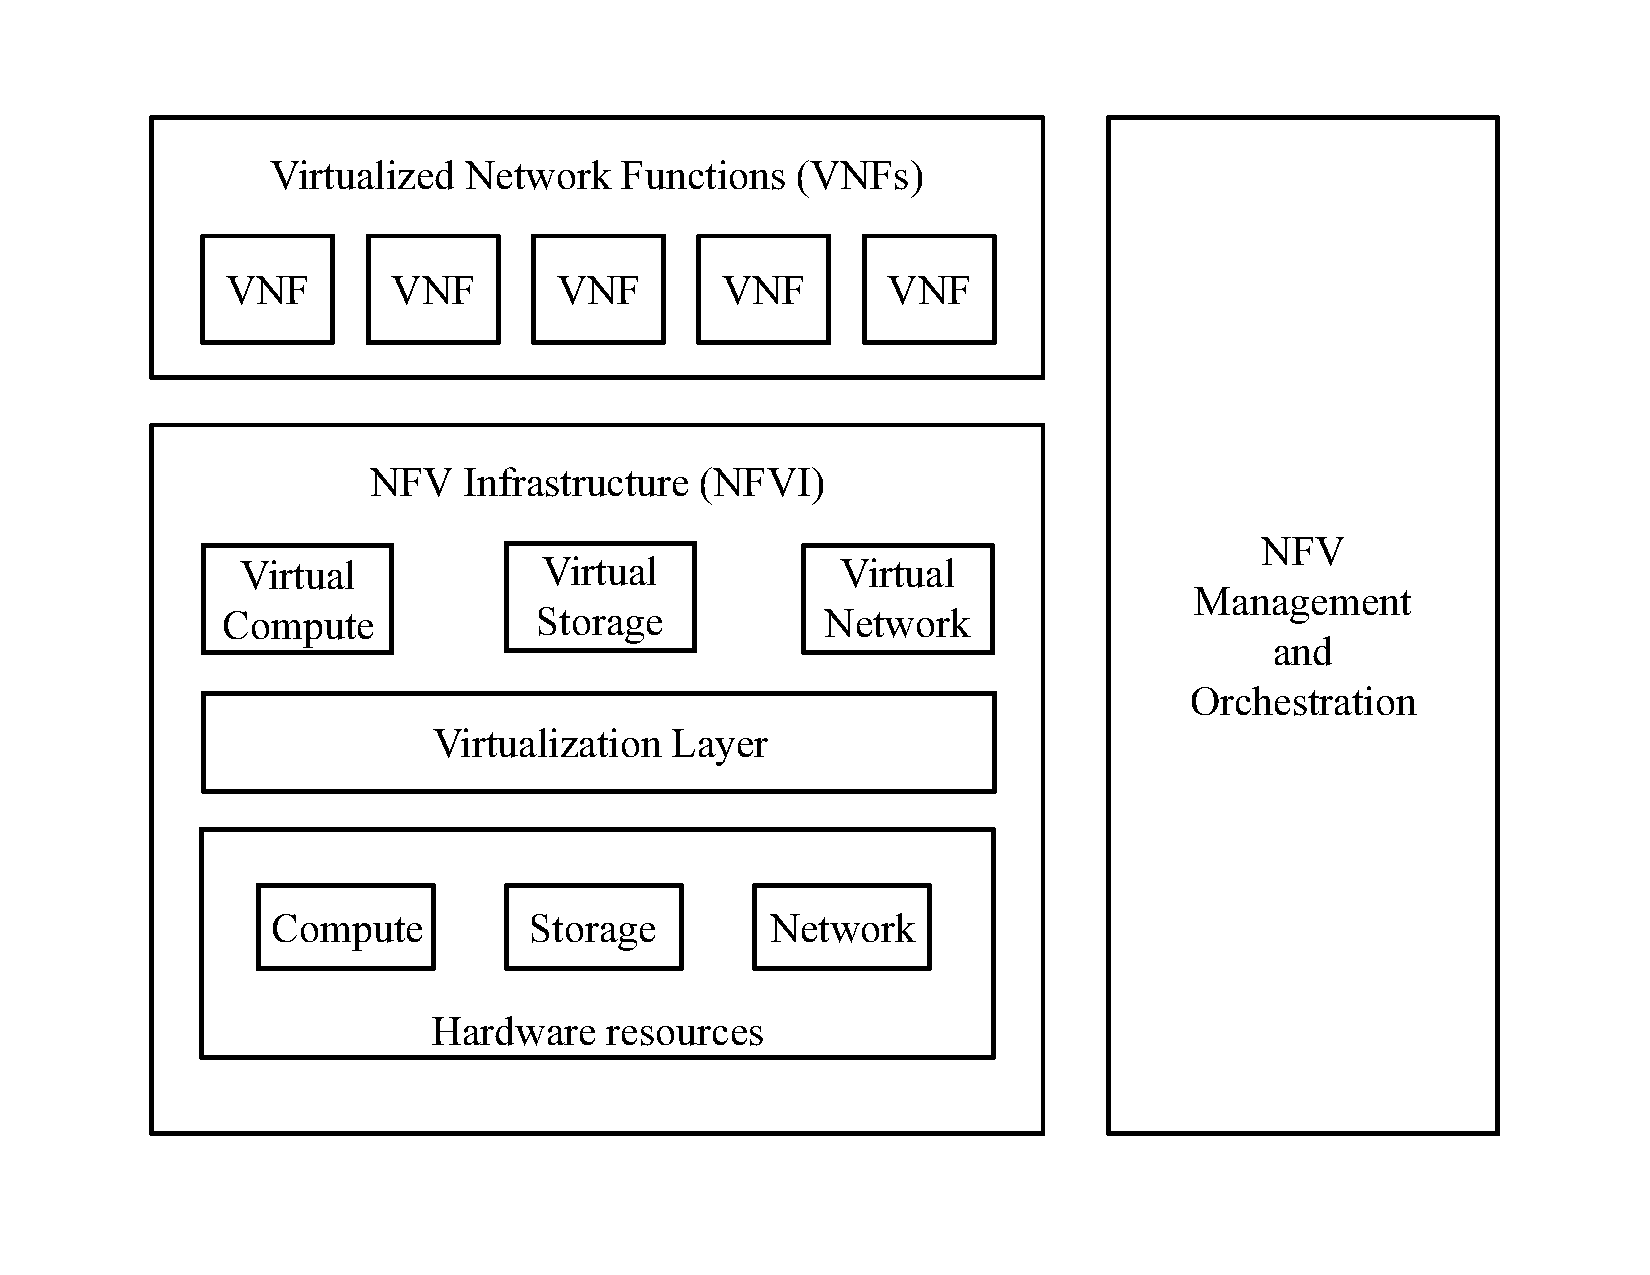
\includegraphics[clip= true, width= \columnwidth]{images/ETSI_Architectural_framework.pdf}
	\caption{High-level NFV framework architecture.}
	\label{fig:etsi_hl_nfv_framework}
\end{figure}

The NFV framework enables dynamic construction and management of VNF instances and the relationships between them in terms of data, control, management, dependencies and other attributes. To this end there are at least three architectural views of VNFs that are centered around different points of view and contexts of a VNF. These perspectives include:
\begin{itemize}
	\item A virtualization deployment/on-boarding angle where the context can be a VM.
	\item A vendor-developed software package perspective where the context can be several inter-connected VMs and a deployment template that describes their attributes.
	\item An operator point of view where the context can be the operation and management of a VNF received in the form of a vendor software package.
\end{itemize}
Within each of the just mentioned contexts, at least the following relations exist between VNFs:
\begin{itemize}
	\item A VNF Set covers the case where the connectivity between VNFs is not specified.
	\item A VNF Forwarding Graph (VNF-FG) covers the case where network connectivity does matter, for instance a chain of VNFs in a web server tier (e.g., firewall, NAT, load balancer)
\end{itemize}

\subsection{Network services in NFV}
An end-to-end network service (e.g., mobile voice/data, Internet access, a virtual private network) can be described by a Network Function Forwarding Graph (NF-FG) of interconnected Network Functions (NFs) and end-points. The termination points and the NFs of the network service are represented as nodes and correspond to devices, applications, and/or physical server applications. A NF-FG can have network function nodes connected by logical links that can be unidirectional, bidirectional, multicast and/or broadcast.
In Figure~\ref{fig:end2end_network_service} is shown an example of an end-to-end network service and the different layers that are involved in its virtualization process. The depicted example offers a clear view of the abstraction (upper part) and how it is remapped on the underlaying physical infrastructure (NFVI). It consists in an end-to-end network service composed of five general purpose VNFs and two termination (end) points. The decoupling of hardware and software in NFV is realized by a virtualization layer. This layer abstracts hardware resources of the NFV Infrastructure.

\begin{figure}[h]
	\centering
	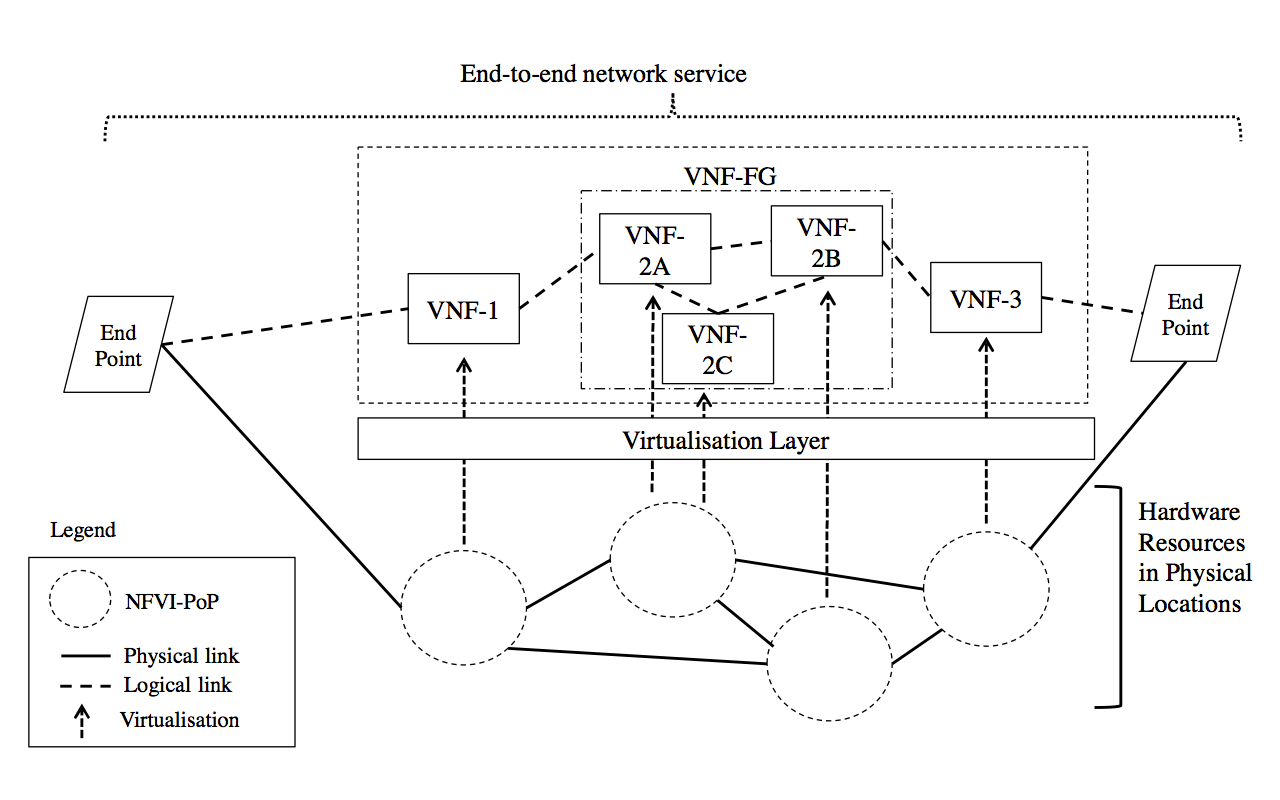
\includegraphics[clip= true, width= \columnwidth, trim=0cm 1cm 1cm 1cm]{images/network_service.png}
	\caption{End-to-end network service with VNFs and nested forwarding graphs example.}
	\label{fig:end2end_network_service}
\end{figure}

\subsection{Architecture of NFV}
The NFV architectural framework identifies functional blocks and the main reference points between such blocks. The functional blocks are:
\begin{itemize}
	\item Virtualized Network Function (VNF).
	\item Element Management System (EMS).
	\item NFV Infrastructure, including:
	\begin{itemize}
		\item Hardware and virtualized resources.
		\item Virtualization Layer.
	\end{itemize}
	\item Virtualized Infrastructure Manager(s).
	\item Orchestrator.
	\item VNF Manager(s).
	\item Service, VNF and Infrastructure Description.
	\item Operations and Business Support Systems (OSS/BSS).
\end{itemize}
Figure \ref{fig:etsi_detailed_nfv_framework} shows the NFV architectural framework depicting the functional blocks and reference points in the NFV framework. The illustrated architectural framework focuses on the functionalities necessary for the virtualization and the consequent operation of operators' networks. It does not specify which network functions should be virtualized, as that is solely a decision of the owner of the network.
\begin{figure}[h]
	\centering
	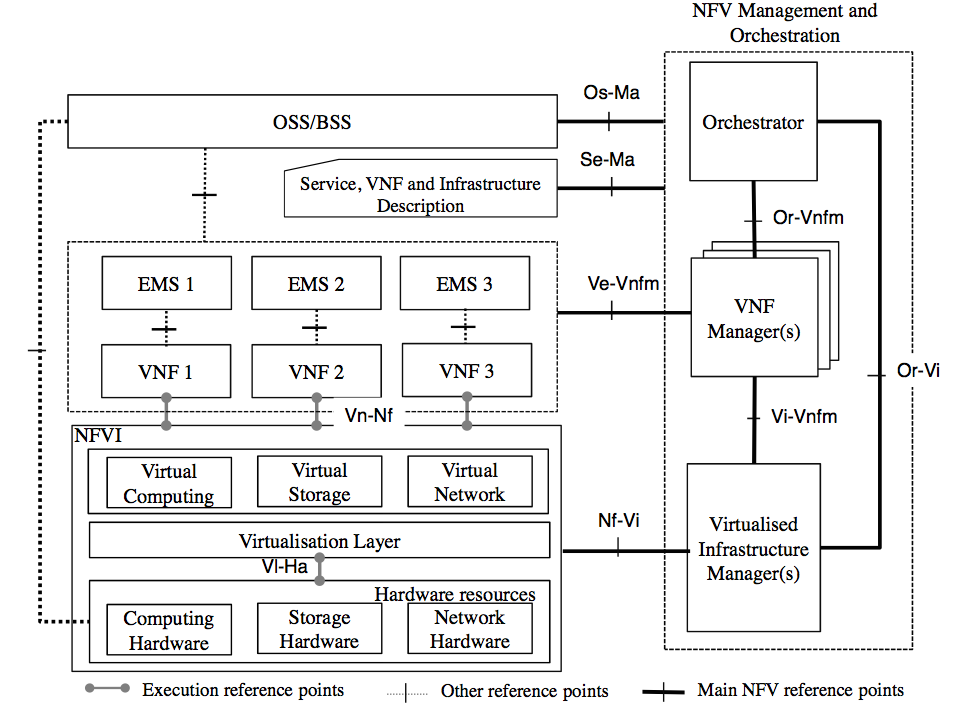
\includegraphics[clip= true, width= \columnwidth]{images/architettura_etsi.png}
	\caption{Detailed NFV framework architecture.}
	\label{fig:etsi_detailed_nfv_framework}
\end{figure}

\subsubsection{Functional blocks}
A functional block defined by the ETSI is the basic unit of a system and consists of:
\begin{itemize}
	\item A set of input interfaces.
	\item A state.
	\item A transfer function.
	\item A set of output interfaces.
\end{itemize}
For the sake of clarity, a view of a functional block is given in Figure~\ref{fig:functional_block}.
\begin{figure}[h]
	\centering
	%left bottom right top
	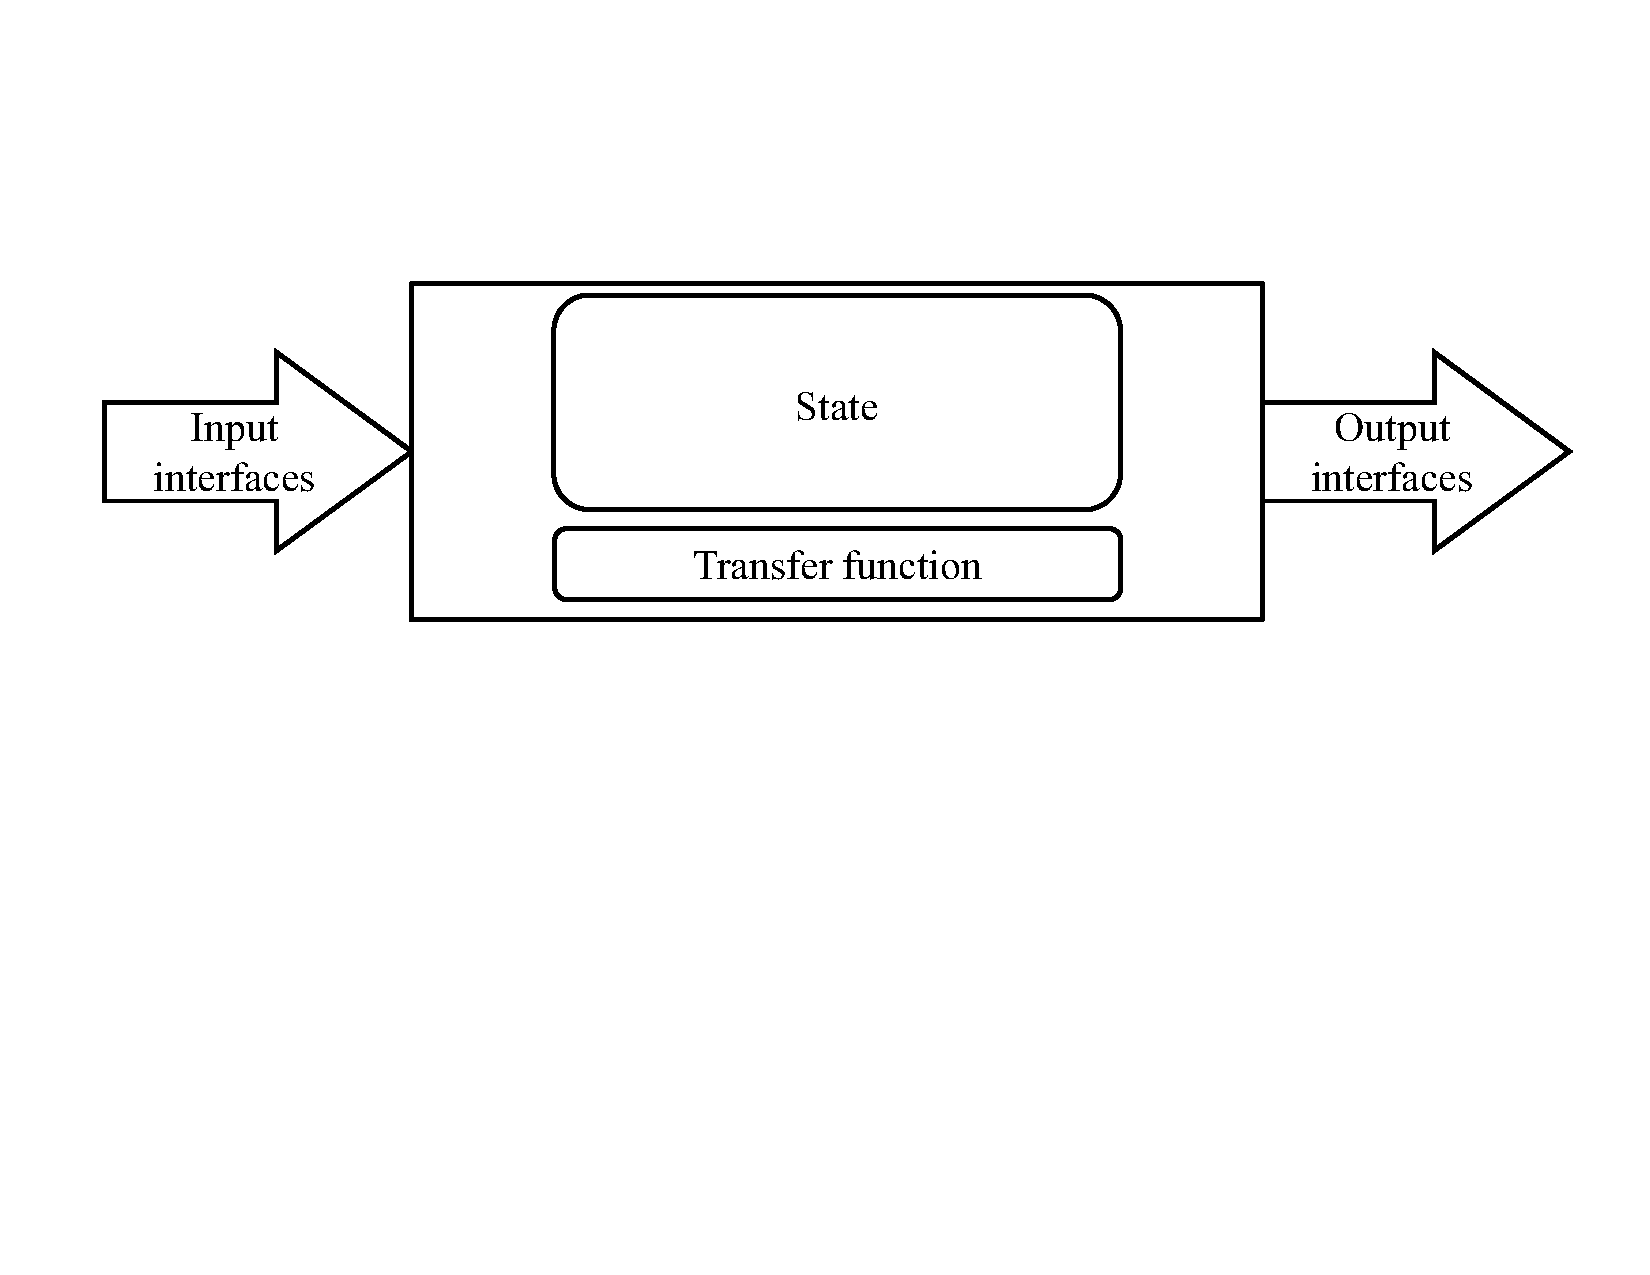
\includegraphics[clip= true, width= \columnwidth, trim=0cm  10cm 0cm 4cm]{images/functional_block.pdf}
	\caption{The fundamentals of a functional block.}
	\label{fig:functional_block}
\end{figure}
A fundamental property of functional blocks is the complete and formal separation of the static from the dynamic. Using a more IT oriented terminology, the input, output, and internal (i.e., state) data structures and all the methods (i.e., the transfer function) are static. They shall not change. Only the values given as input parameters - and therefore the outputs - can change; these values are the only things labeled as dynamic.
Functional blocks are linked together following two fundamental rules:
\begin{itemize}
	\item They can be interconnected, by connecting an output interface of one functional block with the input interface of another functional block.
	\item When a number of functional blocks are interconnected together forming a topology, some input and some output interfaces may remain disconnected. In this case the resulting topology is, in turn, considered as a functional block itself in which the inputs and outputs are the endpoints that remained unlinked in the previous passage. The new obtained functional block follows the very same rules as a standard one.
\end{itemize}

\subsection{Templates}
\label{sec:NFFG}
ETSI introduces five descriptor for deployment and life-cycle management of virtual network functions (VNF) and network services (NS):
\begin{itemize}
	\item Network Service Descriptor (NSD)
	\item VNF Descriptor (VNFD)
	\item VNF Forwarding Graph Descriptor (VNFFGD)
	\item Virtual Link Descriptor (VLD) 
	\item Physical Network Function Descriptor (PNFD) 
\end{itemize}

A \textbf{Network Service Descriptor} is a deployment template for a Network Service referencing all other descriptors which, in turn, describe components that are part of that Network Service.

In addition of containing descriptors, NSD also contains connection points and, optionally, dependencies between VNFs. The connection point is an information element representing the virtual and/or physical interface that offers connectivity between instances of NS, VNF, VNF Componet (VNFC), Physical NF Descriptor (PNF) and a Virtual Link (VL). Examples of virtual and physical interfaces are virtual ports, virtual NIC addresses, physical ports, physical NIC addresses or endpoints of an IP VPN.
The meaning of dependencies between VNFs is quickly explained throughout an example; a function must exist and be connected to the service before another can be initiated/deployed and connected.

A \textbf{VNF Descriptor (VNFD)} is a deployment template which describes the way a VNF has to be deployed and its operational behavior requirements. It is primarily used by the VNF Manager during the process of instantiation and life-cycle management of a VNF instance.

The information provided in the VNFD is also used by the NFV Orchestrator to manage and orchestrate Network Services and virtualized resources all over the NFV Infrastructure. The VNFD also contains information for management and orchestration layer (MANO) functional blocks that allow to establish appropriate virtual links with NFVI between its VNF Component (VNFC) instances or between a VNF instance and the endpoint interface that has to be linked to the other network functions.

A \textbf{VNF Forwarding Graph Descriptor (VNFFGD)} is a deployment template that differs from the others because it takes care of describing the topology of a Network Service (or a portion of it) by referencing  VNFs, Physical NFs (PNF) and Virtual Links that interconnect them. Essentially, it defines the paths that different kind of traffic have to follow and the ordered list of VNFs that they must go through.

A \textbf{Virtual Link Descriptor (VLD)} is a deployment template which describes the resource requirements that are needed for a link that will be used to connect VNFs, PNFs and endpoints of the network service; requirements could be expressed by various link options that are available in the NFVI. The NFV Orchestrator can select an option after consulting the VNFFG to determine the appropriate NFVI to be used. The choice can be based on functionality (e.g., two separated and distinct paths to provide resiliency) and/or other needs (e.g., network physical topology, regulatory requirements, etc.).

Finally, the Physical Network Function Descriptor delineates the connectivity, the interface and key performance indicator\cite{KPI} requirements of virtual links that are terminated on one side by a Physical Network Function(PNF); this flexibility is needed if hardware devices are incorporated in a Network Service, for example to facilitate the transition torward a fully virtualized environment.

% !TEX root = ../thesis.tex
\chapter{Backgroud}
\label{chap:Utilized Tools}

\section{Openstack}
\label{sec:openstack}
\subsection{Overview}
OpenStack\cite{OpenStackwebsite} is an open-source cloud toolkit consisting of a series of interrelated projects that control pools of processing, storage and networking resources in a datacenter.
This project, started in 2010, aims to behave as a datacenter operating system or cloud OS.
As a traditional operating system, a cloud operating system has the main purpose to export an abstraction of the physical hardware but, instead of piloting directly the integrated circuits via drivers as in the single server case, it has the ability to interface itself with an arbitrary number of agents resident over the hypervisor - or virtual machine monitor (VMM) - of each physical server's operating system, in other words it behaves as a manager of hypervisors.
Cloud operating systems simplify the management of a datacenter in which virtual machines are heavily utilized. In fact, they provide a level of abstraction in which all the physical servers are seen and can be managed from a single point.

The OpenStack project aims to provide a centralized interface to be used by datacenter administrators, giving them an overview about resources availability, usage and status and therefore putting them in the position to plan maintenance or provision hardware resizing in order to keep up with the demanded computational power.
Being a commercial product and not only a proof of concept, OpenStack is also engineered to allow the coexistence of administrators and normal users, the firsts are in charge of monitoring the resources availability and manage the infrastructure of the datacenter, providing to the seconds the possibility to instantiate virtual machines and interconnecting them without worrying about configuring the physical infrastructure and the actually available resources.
Normal user is a general term that will refer to an actor that does not have administrative privileges (i.e., he does not have full control over the system); in the case of OpenStack, a user can correspond to either a single person, a department in a company or even to an entire firm that decides to rely on an external infrastructure in where to deploy the virtual servers that provide the services needed for business.
Of course this automation and level of abstraction come at a price which is affordable without any problem in a datacenter environment; on the other hand, in the case of very small amount of physical machines, the overhead is not negligible even if not exaggerate, as can be seen in table~\ref{tbl:components_resource_usage2} (note that the data are taken when the system is at operating speed and many of the OpenStack components works with a caching system). % and further inspected later.
Let's say that in general, when the number of equipments exceeds the few units and the virtual machines creation and deletion volume is high enough to overload the amount of requests that administrators can keep up with, the effort to install the OpenStack system will be well rewarded.

\subsection{General design architecture}
OpenStack has been developed having in mind five guidelines, which are:
\begin{itemize}
    \item Component based architecture, to quickly add new behaviors.
    \item Highly capable of easily scale up/down.
    \item Fault tolerant, isolated processes avoid cascading failures.
    \item Recoverable, failures should be easy to diagnose, debug, and rectify.
    \item Open standards, be a reference implementation for a community-driven API.
\end{itemize}
As mentioned above, OpenStack is not a single project but a pool of independent modules that communicate together, each one in charge of providing one or more functionalities (e.g., computing and network management, authentication, etc).
Modularity has two main benefits: the first one is to permit datacenter administrators to choose what features they want and what they do not, enabling the possibility to offer users different typologies of service; the second advantage is the interchangeability of modules that are designed for the same purpose (e.g., network management) so that an administrator can pick the module that suits the best or even write one by himself from scratch.
The majority of modules are, in turn, split into submodules and designed to allow plugging in special purpose add-ons written to accomplish specific tasks or made the module behave in a certain desired way.

\subsection{Physical architecture}
The deployment of OpenStack requires a total amount of three logically separated entities that can be remapped into one or more physical machines.
These three entities are generally referred as the following:
\begin{itemize}
    \item \textbf{Controller node}.
    \item \textbf{Compute node}.
    \item \textbf{Network node}.
\end{itemize}

In the \textbf{Controller node} resides a set of supporting services, basic (or core) components and a series of optional features.
Supporting services are not properly OpenStack components but are necessary for its operations; two of these components are the database management system (e.g., MySQL\cite{mysql}) for persistent storage and the message broker (e.g., RabbitMQ\cite{rabbitmq}) for modules intercommunication. Having them in the controller node is not mandatory but since the major share of requests to this components comes from services also resident in the control node, delays due to the network are eliminated.
Basic components are all those OpenStack modules that provide the very basic functionalities and that will become the "brain" in charge of managing the whole infrastructure.
In addition, in the controller node can be installed optional components that are not crucial but offer useful functionalities such as Ceilometer. Ceilometer is the OpenStack telemetry service that tracks resources usage aggregated by user, giving the possibility to manage billing in case of a datacenter offered as a service.
Another optional component is the orchestrator known as Heat that is in charge of communicating with both the network and the compute manager.
The controller node needs to communicate directly with all the other nodes (via a management interface) to dispatch commands and receive updates from them as depicted in Figure~\ref{fig:os_cloud} and further detailed in Figure~\ref{fig:OSarchitecture}.

The \textbf{Compute node} is in charge of actually hosting the virtual machines. This node is a single physical server and, if we consider the controller node as the brain of OpenStack, this compute node can be seen as the muscles. Since all the control services are hosted in the controller node, the amount of software required to be installed in the compute node is minimal, saving computing resources for the virtual instances that will be deployed on it. The only pieces of code required are an agent that communicates with the local hypervisor and - optionally - another agent that takes care of accepting particular commands to provide traffic isolation between users. In addition, in case of usage of optional services that require a distributed agent to retrieve statistics, also these agents run in the compute node.
Compute nodes are connected to the controller node in order to receive instructions, and have a separated network interface, referenced as \texttt{"instance tunnel"} in Figure~\ref{fig:OSarchitecture}, to communicate with each other, permitting to users' VMs to exchange traffic.
An edge of this network of Compute nodes there is the Network node.

The \textbf{Network node} is the border between the OpenStack domain and the outside world; in particular, is in charge of being the only node that has the capability to connect to the external network and let VMs traffic in and out to the Internet. It is also connected to the Controller node to receive commands. VMs are not instantiated in this frontier component, but it runs agents that will be in charge of providing basilar network services such as network address translation (NAT), ip assignation (DHCP) and privacy policies via a firewall.
\begin{table}[h]
\begin{tabular}{l|l|}
\cline{2-2}
                                                          & RAM {[}MB{]} \\ \hline
\multicolumn{1}{|l|}{\textbf{Controller node - full installation}} & 2100         \\ \hline
\multicolumn{1}{|l|}{\textbf{Controller node - minimal installation}}                                   & 1500         \\ \hline
\multicolumn{1}{|l|}{\textbf{Compute node}}                                   & 590          \\ \hline
\multicolumn{1}{|l|}{\textbf{Network node}}                                   & 250          \\ \hline
\end{tabular}
\centering
\caption{OpenStack nodes - resource analysis.}
\label{tbl:components_resource_usage2}
\end{table}

\label{a:br_section}
In the classic architecture of an OpenStack domain, each compute node have two virtual switches that can either be linux bridges, openvswitches\cite{ovswebsite} or xDPd\cite{xdpdwebsite}: one for attaching the VMs (generally called br-int) and the other (referred as br-net or br-tun) to create virtual tunnels with the other compute nodes, establishing a full mesh network that will carry packets from one server to another, thus making the intermediate network infrastructure completely transparent. The Network node, in addition to these two bridges, has another one (usually referred as br-ex) to which is bridged the physical network interface card (NIC) that has access to the Internet. As said before, the network node does not host virtual instances but instead it hosts network services; these services are attached to the br-int.
The br-int and the br-ex in the Network node are not linked in any way so that neither traffic can leave the inside of the datacenter, nor outside packets can enter the private network, unless a specific service (a router) is deployed and linked with two virtual interfaces, one connected to each of the two software switches.

Logical schemes for better understanding the complex architecture is provided in Figure~\ref{fig:os_cloud},~\ref{fig:OSarchitecture} and~\ref{fig:os_coud_with_br}, more details of the depicted services are available in section \ref{a:main_components}.
\begin{figure}[h]
	\centering
	% left bottom right top
	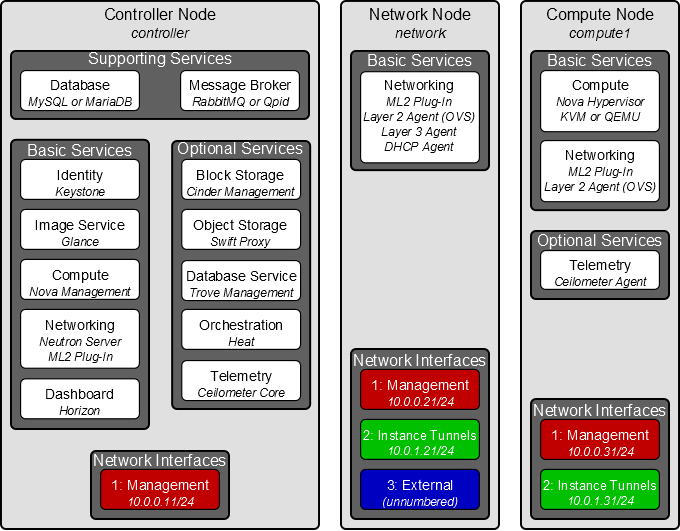
\includegraphics[clip= true, width=0.8 \columnwidth]{images/openstack_nodes.png}
	\caption{OpenStack logical nodes - services and interfaces.}
	\label{fig:OSarchitecture}
\end{figure}
\begin{figure}[h]
	\centering
	% left bottom right top
	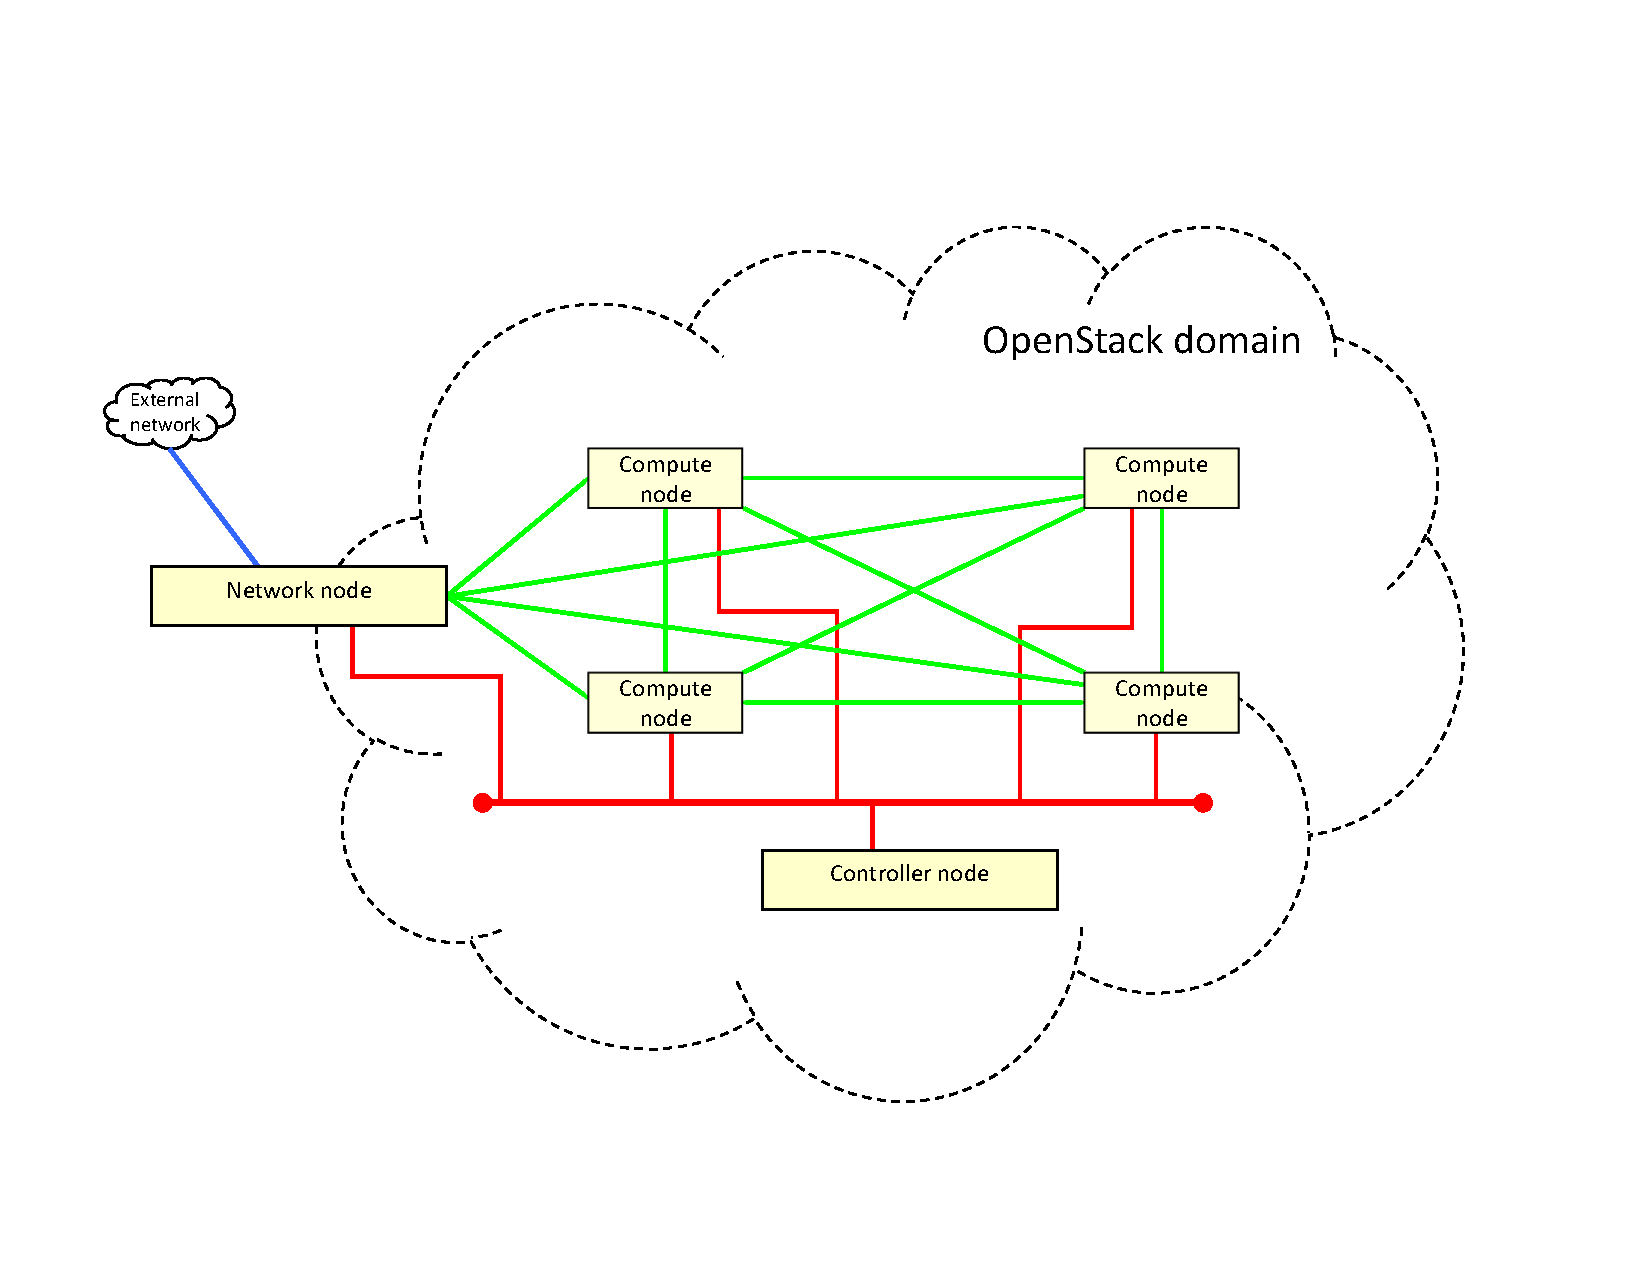
\includegraphics[clip= true, width= \columnwidth, trim=0cm 1cm 0cm 3cm]{images/os_cloud.pdf}
	\caption{OpenStack domain - Nodes interconnections.}
	\label{fig:os_cloud}
\end{figure}
\begin{figure}[h]
	\centering
	% left bottom right top
	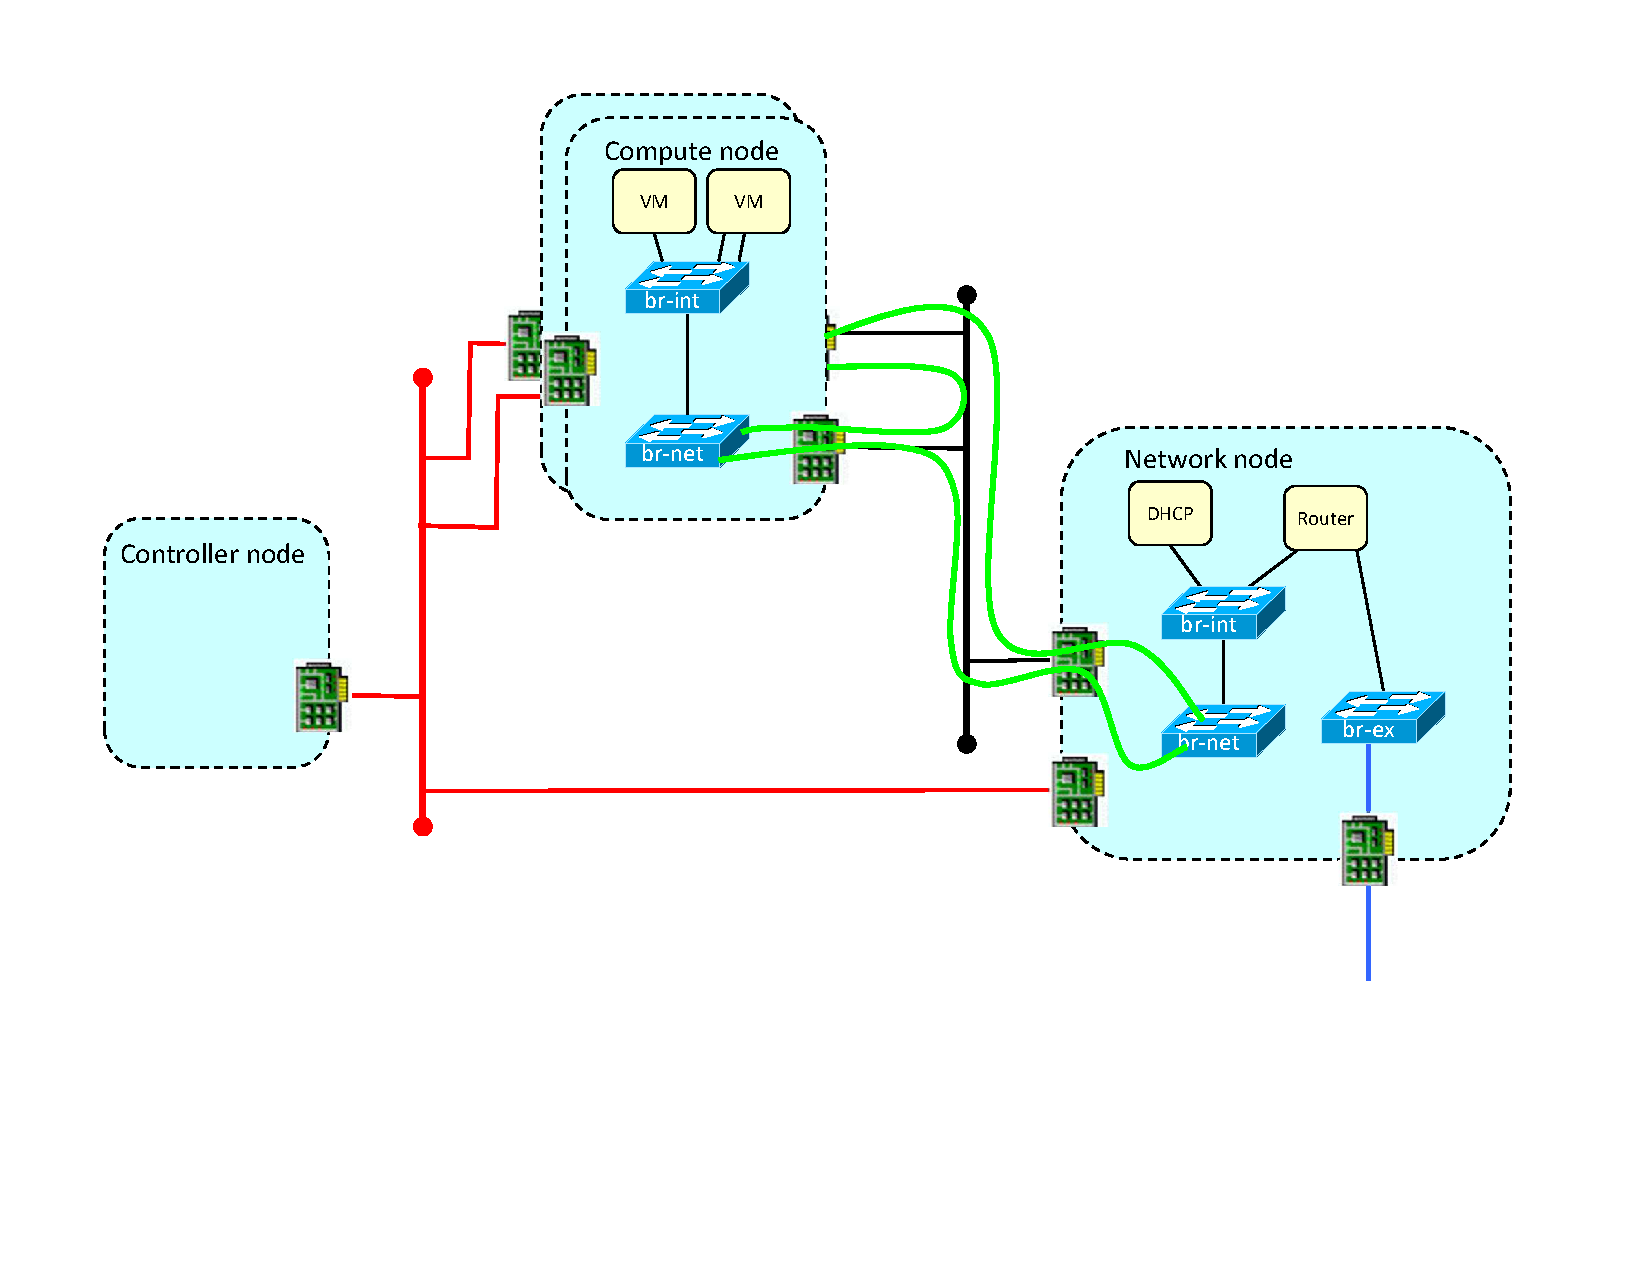
\includegraphics[clip= true, width= \columnwidth, trim=0cm 3cm 0cm 0cm]{images/os_cloud_with_br.pdf}
	\caption{OpenStack domain - Nodes interconnections in detail.}
	\label{fig:os_coud_with_br}
\end{figure}

%aggregation of logical entities
The logical architecture just described, depending on the size and computing power of the datacenter, can be remapped in various ways; in particular, the three entities can be aggregated as the administrator likes at installation time: a common deployment is to devolve one server serving as controller node and one as a network node, plus a number of compute nodes. However, in case of a very small datacenter in which there are just some physical machines nodes can be collapsed, even, OpenStack can be used to manage just one server; in this particular case one single machine will have all the three entities at the same time. Evidently the last example is a critical situation in which the introduced overhead is really influencing the performance, therefore this kind of configuration is useful only for developing and testing purposes.

\subsection{Main components}
\label{a:main_components}
OpenStack modules (called services in the follows) communicate together either via RESTful API or via a message broker server and may have the need to query a database. Additionally, in case of a datacenter as a service provided to external users, OpenStack offers a web interface - the Horizon dashboard - that requires a web server in order to serve users' requests.
These three additional services are not part of the core components of OpenStack but, based on the standard configuration, they are necessary and essential for the system to work properly.
As visible in Figure~\ref{fig:OS_components_interraction_logical}, which represents the main OpenStack components and their interactions, the services are clearly separated by functionality. From the image, it is also evident that two components are more involved in communications compared to the others. These two components are the previously cited (optional) dashboard and the identity service, which provides authentication to both services and users.
\begin{figure}[h]
	\centering
	% left bottom right top
	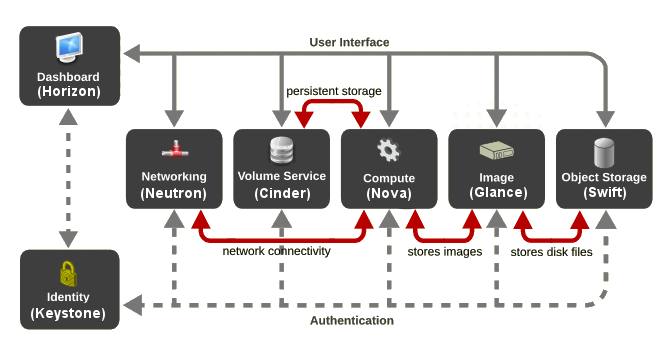
\includegraphics[clip= true, width= \columnwidth]{images/openstack_core_components.png}
	\caption{Internal components interaction.}
	\label{fig:OS_components_interraction_logical}
\end{figure}

\subsubsection{Identity - Keystone}
\label{sec:keystone}
As a distributed environment, the system has to provide secure access and hence both users and services must authenticate themselves before performing any operation.
OpenStack developers wrote a specific service called \textbf{Keystone} for this purpose; it stores username and password for each authorized user/service, the authorization process involves obtaining a token to be used later to perform requests to other services. The general concept behind a token-based authentication system is simple: it allows users to enter their username and password in order to obtain a token, which enables them to fetch a specific resource - without using their username and password again. Once the token has been obtained, the user can use the token, which offers access to a specific resource for a time period. Identity also correlate a user to its role in the system, and the visibility of resources. Administrators are able to see everything that is going on in the system, while a common user can only see the virtual resources he created.
This separation of group belonging in keystone is called role and is used by other services to check whether the user is authorized or not to perform such operation, basically defining a sandbox for each user so that anyone can only see what he is authorized to.
Alongside the user concept, keystone defines three fundamental terms which are group, tenant (or project) and domain; in this way rules can be associated to them instead of directly to a user. These terms are remapped to internal data-types; here below a list of Keystone resources is given alongside with a brief description and usage:
\begin{itemize}
	\item User: contains account credentials and is associated with one or more projects or domains.
	\item Group: a collection of users; it is associated with one or more projects or domains.
	\item Project (Tenant): unit of ownership in OpenStack; it contains one or more users part of a Group.
	\item Domain: contains users, groups and projects.
	\item Role: a piece of metadata associated with many user-project pairs.
	\item Token: identify credential related to a user or to a user-project pair.
	\item Extras: bucket of key-value metadata associated with a user-project pair; it is intended to provide a method to send extra fields in a REST call without changing its interface.
	\item Rule: describes a set of requirements for performing an action.
\end{itemize}
Since credentials are generally built from the user metadata in the \texttt{"extras"} field of the Identity API, adding a \texttt{"role"} to a user just means to add the role to the metadata.
Data-types are used inside keystone to provide a set of services that are exposed to users via one or more HTTP endpoints:
\begin{itemize}
	\item Identity: this service is intended to provide authentication, credential validation and data about Users, Groups, Projects, Domains and Roles, as well as any associated metadata. In the basic case all these data is managed directly by the service itself that exposes all the CRUD methods associated with the data.
	\item Token: service that validates and manages tokens that are used when performing requests, typically to other services; a token is created once a user credentials have been verified.
	\item Catalog: which provides a registry used for endpoint discovery, this permits to know how to contact all the other services.
	\item Policy: this service provides a rule-based authorization engine and the associated rule management interface.
\end{itemize}
Policies based on a set of rules can be specified for each OpenStack component; all components have their own \textit{"policy.json"} file that permits to associate rules to all Openstack service actions. In listing~\ref{lst:nova_policy} is an example of policy.json file of Compute service (Nova) in which is defined - lines 14 and 15 - a policy that only permits to the user identified as the owner or an administrator to start or stop a VM, meaning that someone that shares a project with the previous user is not allowed to manage a VM not belonging to him.
\lstinputlisting[label=lst:nova_policy, language=python, caption={policy.json file relative to the Nova service.}]{code/nova_policy.json}

\begin{comment}
Each one of the Keystone services listed above can potentially be connected to a different backend, this is done to allow Keystone to fit a variety of environments and needs. The most popular choice is a SQL based one that leverages SQLAlchemy to store data persistently. If this solution is adopted, the keystone-manage command can be used to introspect the backend and, by running the \texttt{"db\_sync()"} subcommand, to upgrade the database schema. In substitution to this first classical solution, a Lightweight Directory Access Protocol (LDAP) backend can be used to store users and projects in separate subtrees, roles then are recorded as entries under the projects they belong to. The possibility to choose between different kinds of backend is mainly available thanks to the structure that the majority of OpenStack projects have, that is an abstract class defines basic interactions and primitives callable by frontend services, these functions are then implemented inside a set of special purpose classes, each one dedicated to manage a specific storage system. Administrators can then specify which backend they want and are going to use inserting a proper entry into the dedicated configuration file section.
As well as the backends, OpenStack has a common way to manage the API call and keystone makes no exception. As in other services, an HTTP front-end is exported by using the python WSGI interface. HTTP endpoints are made up of pipelines of WSGI middleware that, in turn, use a subclass called \texttt{"ComposingRouter"} that takes care of linking URLs to one of the defined controllers; within each controller, one or more managers are loaded. Managers are thin wrapper classes in charge of loading the appropriate service driver based on the keystone configuration.
\end{comment}

\subsubsection{Storage - Cinder, Swift and Glance}
\label{sec:openstack_storage}
Numerous projects have been started focusing on different specific purposes related to disk management.

\textbf{Block storage} - known as Cinder - allows to dynamically attach additional disks to virtual machine instances. This ability allows to scale up the available disk size of a specific virtual machine avoiding the need to destroy and recreate the same instance only with more storage space.

\textbf{Object storage} - codename Swift - is meant to manage a distributed, API-accessible storage platform that can be integrated directly into applications or used for backup, archiving and data retention. This comes particularly handy in the typical scenario of a datacenter where the computing power is kept separated from the large hard drives where data reside. Swift provides similar functionalities that a network-attached storage (NAS) does.

Unlike the two above cited services that are not identified as OpenStack core components, the \textbf{image service} (Glance) is very important and provides the ability to retrieve, copy and snapshot a server image and store it leveraging the others storage services or interacting directly with the local file system.
Images can be uploaded in various formats and pinned as public or stay private, meaning that they can be used only by the user that created them.
A service that takes care to allow customers to manage their own base images and create snapshots is crucial to provide a flexible customizable experience to end users.
Glance has a RESTful API that allows querying for snapshot's metadata as well as retrieval of the actual image.
This function is crucial in the moment of instantiation of a virtual machine since at startup time a bootable disk is essential.
Associating information to disk image is also trivial at instantiation time when resources are reserved and assigned to a virtual machine. In this moment is essential to check if the given resource quotas are enough to support the chosen image and therefore make the VM work correctly.

\subsubsection{Computing - Nova}
\label{sec:nova}
The compute part is one of the critical services of OpenStack, being the one that actually makes virtual machine instances run.
It is designed to manage and automate pools of compute resources and can work with widely available virtualization technologies, as well as baremetal and high-performance computing (HPC) configurations.
Given its complexity, this component, in turn, has been divided into submodules, each one in charge of one particular task.
\begin{figure}[h]
	\centering
	% left bottom right top
	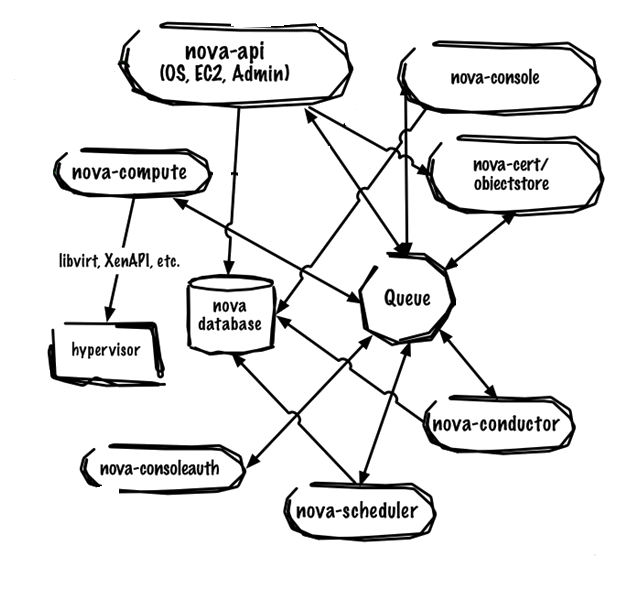
\includegraphics[clip= true, width= 0.6 \columnwidth]{images/nova_components.png}
	\caption{Nova components and interactions.}
	\label{fig:OSnovalogical}
\end{figure}
The two components of particular interest are the compute and the scheduler submodules.
The former is a worker daemon called \textbf{nova-compute} and resides in each compute node. It is in charge of creating and terminating virtual instances through hypervisor APIs, for example XenAPI for XenServer/XCP, VMwareAPI for VMware, libvirt for KVM and others as depicted in Figure~\ref{fig:OSnovacompute}.
Given that KVM and XenServer are popular choices for hypervisor technology and recommended for most use cases, OpenStack also wants to meet the needs of those administrators that do not have at their disposal a large computational power and might want to use a linux container technology such as LXC, and wish to minimize virtualization overhead and achieve greater efficiency and performance. In addition to different hypervisors, OpenStack supports Intel, ARM and other hardware architectures.
The nova-compute agent is also in charge of letting the other nova submodules located in the controller node aware of its existence and status, this job is done by sending periodical messages to the message broker service.
\begin{figure}[h]
	\centering
	% left bottom right top
	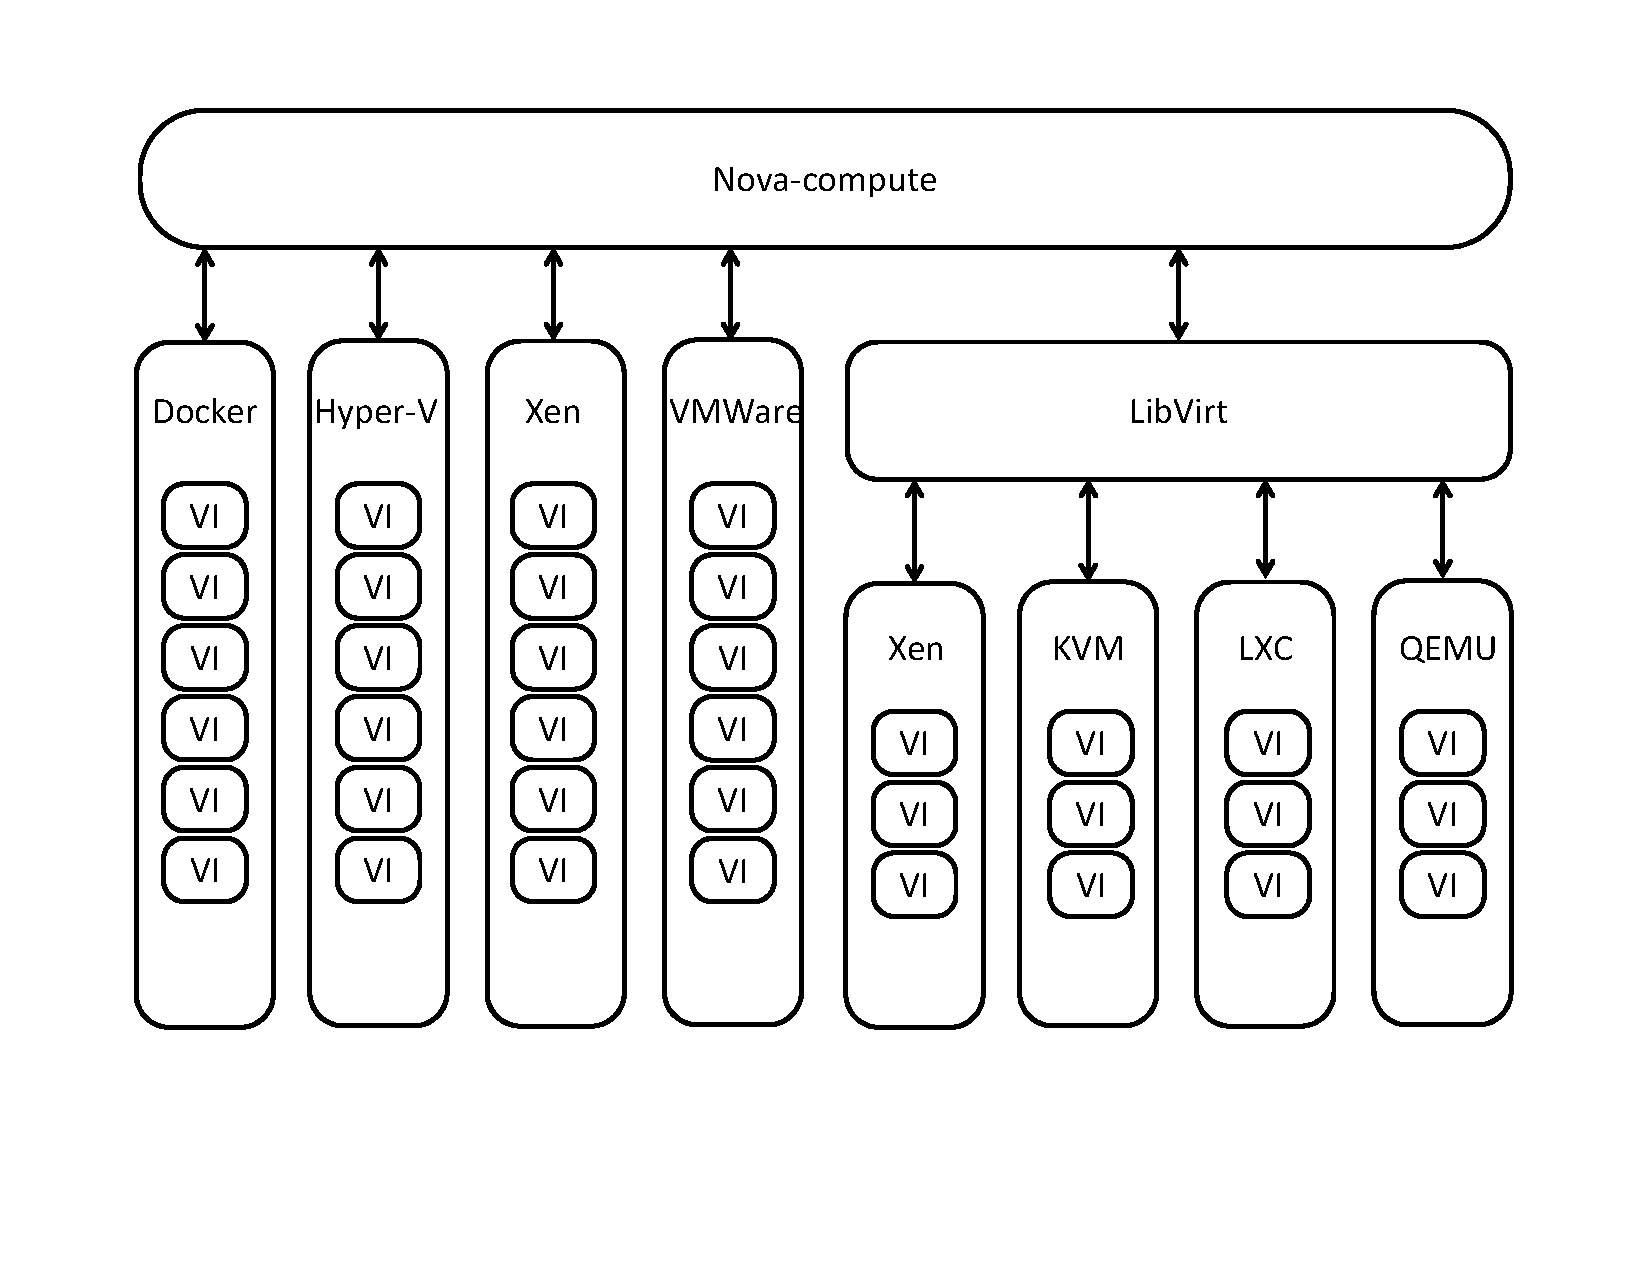
\includegraphics[clip= true, width=0.8 \columnwidth]{images/nova-compute.pdf}
	\caption{Nova compute hypervisors support.}
	\label{fig:OSnovacompute}
\end{figure}
In the controller node are located both the module that manages requests (\textbf{nova-api}) and the \textbf{nova-scheduler}, which is in charge of choosing where the virtual machines are going to be instantiated.
The scheduler submodule is very important and valuable for an administrator that wants to maximize the efficiency of the entire system.
As default, OpenStack comes with an algorithm that takes decisions in a two-steps process called filter and weight, a representation of this sequence of events is given in Figure~\ref{fig:OSnovascheduler}.
In the first step, it excludes from all the available hosts, the ones that do not meet specific requirements (e.g., free resources, architecture, hypervisor, etc), while in the second step all feasible hosts remained after the filtering are weighed according to a predefined cost function. The filter manager module is explicitly thought in a way that new constraints can be defined to further skim the pickable nova-compute module.
On the contrary of the filter module, the weighing function is customizable but unique so it has to be tuned with consciousness; its only purpose is to model each remaining host with a number, then the host with the highest value is chosen and the command to instantiate the virtual machine is dispatched to the corresponding nova-compute agent.
Both filter and weight steps take into consideration the information - generally referred as host status - exported by each nova-compute that typically consists in free resource availability.
\begin{figure}[h]
	\centering
	% left bottom right top
	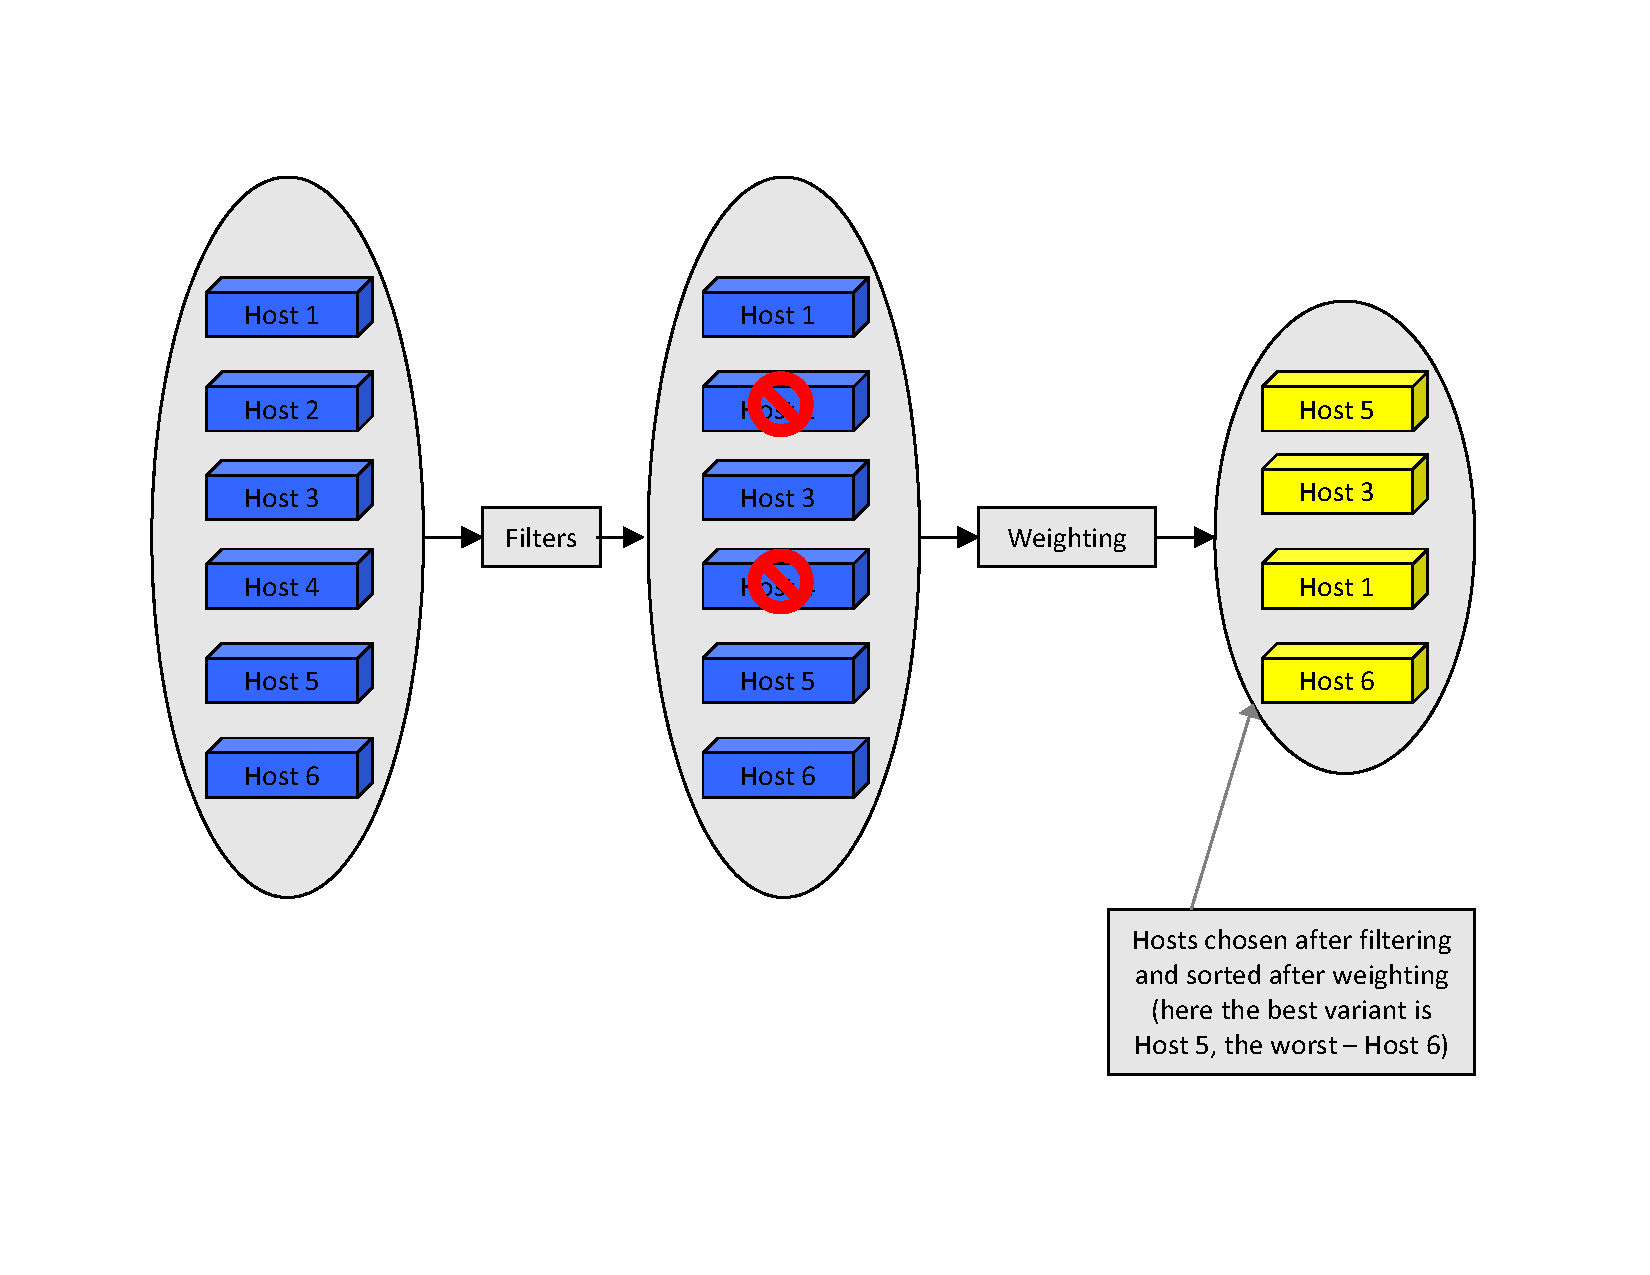
\includegraphics[clip= true, width= \columnwidth, trim=0cm 3cm 0cm 3cm]{images/nova-filter-weight.pdf}
	\caption{Filter and weight scheduling process.}
	\label{fig:OSnovascheduler}
\end{figure}

\subsubsection{Network - Neutron}
\label{sec:neutron}
As well as Nova, \textbf{Neutron} is also a core component of OpenStack and it is in charge of managing the network that interconnects the virtual machines.
Actually, it would be more correct to say that it is in charge of managing the virtual overlay network that interconnects the virtual machines as it does not have any knowledge about the physical interconnections between compute nodes.
Neutron, formerly known as Quantum, provides users an abstraction that allow them to interconnect their own virtual machines and define some basic network services such as router, dynamic host configuration protocol (DHCP), firewall and virtual private network (VPN) terminator, decide which IP address assign to a VM and choose whether a VM is reachable from the Internet or not.
When a user decides to modify his own network topology or performs operations such as launching or stopping a virtual machine, Neutron quickly reconfigures the virtual switches - br-int, br-tun/br-net - to provide connectivity and isolation.
In order to understand the level of abstraction provided by this component, it is necessary to look at the network at three different levels.
First comes the lower layer, composed of the physical equipments such as Ethernet cables, optical fibers and hardware switches; on top of this, a full mesh of generic routing encapsulation (GRE) tunnels are established between all the br-tun/br-net virtual switches infrastructure explained in section \ref{a:br_section}.
Over this layer lays the actual user defined networks, modeled with virtual local area network (VLAN) and carrying the traffic through the GRE tunnels.
This behavior is modifiable by intervening on the configuration files of Neutron and therefore adapting this service to better suits the datacenter communication infrastructure.
Being this flexible requires Neutron to have a structure as the one in Figure~\ref{fig:neutron_structure}, where five levels are indicated.
\begin{figure}[h]
	\centering
	% left bottom right top
	\includegraphics[clip= true, width= \columnwidth, page=53, trim=0cm 8cm 0cm 0cm ]{images/Pictures_definitivo.pdf}
	\caption{Neutron architecture.}
	\label{fig:neutron_structure}
\end{figure}
The first two from the top are in charge of receiving requests, serialize and transform them into objects that models Neutron resources. The user is provided with a set of primitive to create his own network topology; these primitives are nothing less than Neutron resources that are:
\begin{itemize}
\label{neutronresourcelist}
    \item Network - defines a L2 broadcast domain.
    \item Subnet - in a network, it defines an IP address range
    \item Port - in a subnet, it defines an attachment point for either a VM, a router or a firewall.
\end{itemize}
Scrolling down the architectural stack (shown in figure~\ref{fig:neutron_structure}), there is the Modular Layer 2 plug-in (ML2), which is in charge of keeping the internal status of the network service to provide robustness and recoverability after a major failure of the neutron component. It also fulfill the \texttt{"GET"} requests that are useful for example to the dashboard to represent in a graphical manner all the information relative to the user's network topology.
Below the ML2 there are two managers layer that are in charge of dispatching requests to type and mechanism driver modules.
Both the drivers kind are intended to provide and implement per user and - if required - per user's network isolation. Let's say that the type driver decides the standard that is going to be used and the mechanism is in charge of implementing it.
Type drivers are pluggable modules in which information about how to guarantee isolation are added to the Neutron objects. The modified object is then returned to the third level of the stack that finally passes it to the other manager which is in charge of dispatching the received object to one or more drivers.
A mechanism driver is specifically designed to communicate with a particular virtual switch that resides in the compute nodes. This component is crucial and each vendor can easily develop one that remaps Neutron objects (listed in~\ref{neutronresourcelist}) to commands specific to its device; OpenStack comes with already a lot of drivers from which to choose; for example the one for openvswitch, linuxbridge and the one developed expressly for the integration with OpenDaylight which will be described in section \ref{sec:opendaylight}.
Mechanism drivers are actually called twice each time a resource is created, updated or deleted: before the ML2 database operation and then again after that the data-base transaction is concluded successfully.
This double call allows to the mechanism driver to prepare and check the feasibility of the operation and only after it the grant from the upper layer, the operation is actually performed.
To summarize, Neutron other than providing connectivity between VMs, also establishes user isolation in a way that inter-user communication can happen only via a public network defined by the administrator for this specific purpose.

\subsubsection{Orchestration - Heat}
\textbf{Heat} is the main project in the OpenStack Orchestration program. It implements an engine to launch multiple composite cloud applications based on templates in the form of text files that can be treated like code. It aims to export a unique-common API usable by the user to instantiate a complete network topology comprehensive of virtual machines in the form of a template making just one call; the Heat engine then takes care of translating such template into calls for both Nova and Neutron. In order to improve performance, all these calls will be made in parallel unless dependencies between resources are implicitly or explicitly specified. As an example of implicit dependency let's consider neutron resources listed in \ref{neutronresourcelist}: a Neutron port attached to a network can exist only if that specific network has already been created.
On the other hand, as explicit dependence the user can point out that a virtual machine must be created before another one - a valid motif can be that the first VM provides services without which the second one cannot boot correctly.
Another useful feature is the management of updates.
When a request is received by Heat and it contains a reference to an already instantiated template, the engine is able to understand what is changed between the allocated resources and the ones present in the request - this is done similarly to the \texttt{"diff"} unix/linux command.
Once this task has come to an end, the creation, modification and/or deletion of resources will be handled; the new ones will be created and the no more needed can be deleted.
For what concerns the update of a resource, Heat allows two ways of behavior. The first one is to rawly destroy the elder and then create a new one with the up-to-date characteristics. A more sophisticated approach is to define in each service the way to handle the update locally (e.g., change the static ip address of a port), however this is not always possible - an example is the case of changing the disk image of a VM.

\subsubsection{Dashboard - Horizon}
Usability is essential in complex systems, hence programmers typically offer a user friendly interface, avoiding the unexperienced users the pain of going through a complex command line tool.
Under this aspect, OpenStack is not an exception and provides a well structured web dashboard called Horizon, from which administrators can monitor the system and users can easily perform operations that otherwise require a long list of command-line inputs.
The dashboard follows the OpenStack's main concept of abstraction and models VMs, networks and network services in a way that even an unexperienced user can easily understand. In Figure~\ref{fig:OSdashboard} is given a screen-shot of what a user sees when a simple topology is deployed. As is evident from the image, there is no indication about the physical location of the VMs (VM1, VM2, VM3), the service (Router) and other user instances.
\begin{figure}[h]
	\centering
	% left bottom right top
	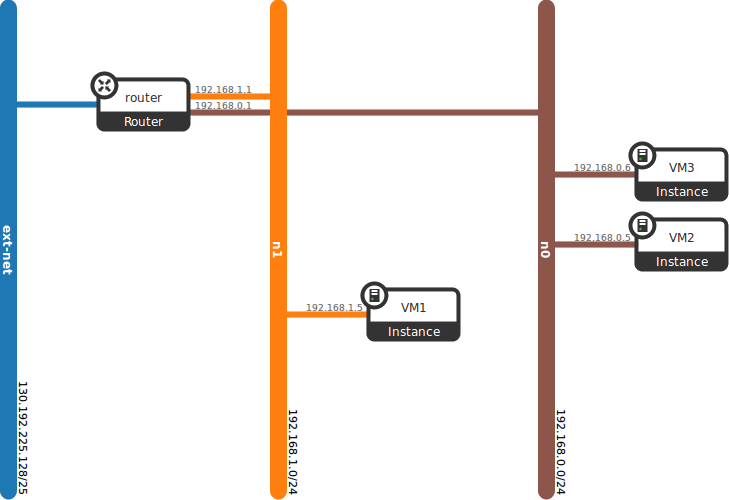
\includegraphics[clip= true, width=0.9 \columnwidth]{images/neutron-topology-example.png}
	\caption{Dashboard view of network topology design with VMs.}
	\label{fig:OSdashboard}
\end{figure}

\subsubsection{Command line clients}
Since all services are meant to receive commands via REST API, OpenStack developers have produced a command-line based client for each project that automates otherwise pedantic operation and complex typing of unicode strings.
These clients perform a series of cURL requests to obtain the required result.
As an example, consider that a user that wants a list of all his virtual machines with some details, using the client, it is easy: just type \texttt{"nova list"}. To achieve the same result, it is mandatory to acquire an authentication token, then use it to query the nova-api and obtain the list of instances. If more details are required, a request for each machine has to be dispatched.
Other than automation, clients provide also data presentation so that instead of receiving responses in form of raw JSON or XML, better-looking and compact tables are displayed.

\subsection{OpenStack towards NFV}
The OpenStack community continues to grow and the number of companies that decide to adopt the open-source solution is constantly augmenting. As it is easy to imagine, these companies work in different fields and have various needs. Keep up with all the requests of new features implementations is almost impossible but the community does its best to at least try. In this optic a new squad, called NFV team, is trying to propose new solutions that should be integrated into OpenStack to better support network function virtualization.
As stated in their official page\cite{NFVteam}, their mission aims to define the use cases, identify and prioritize the requirements that are needed to run Network Function Virtualization workloads on top of OpenStack. This work includes identifying functional gaps, creating blueprints, submitting and reviewing patches to the relevant OpenStack projects and tracking their completion in support of NFV. The requirements expressed by this group should be made so that each of them have a test case which can be verified using an open-source implementation. This ensures that tests can be done without any special hardware or proprietary software, which is key for continuous integration tests in the OpenStack gate. If special setups are required which cannot be reproduced on the standard OpenStack gate, the use cases proponent will have to provide a 3rd party CI setup, accessible by OpenStack infra, which will be used to validate developments against. All the proposals they have ever made can be found on their website\cite{NFVteam} along with their statuses. Looking at the number of active blueprints it can be seen that as a group they are very active so there is quite the possibility their work towards a NFV fully-capable OpenStack will lead to nice results. As a down side, each one of their proposition has to be discussed, reviewed,validated, implemented and finally tested. It is evident that such procedure requires time, also it has to be compatible with all the already existent features.
As an example, let's take the \textit{Services Insertion, Chaining and Steering}\cite{neutronsteeringofficial} extension they proposed for the neutron module. Taking a look at the white-board it can be easily seen the time it is required to finally come to a working implementation; in fact it the proposal came up on late 2013 and as far as October, the 13th 2014 this project still has not been marked as approved.
Even if its purpose is quite similar to the FlowRule abstraction, this proposed extension has evolved during the year coming to look more like the ETSI service chain instead of appearing like an OpenFlow rule as the FlowRule does.
Instead of defining a port-to-port connection with matching rules, they decided to introduce two kinds of resources: \textit{ports chain} and \textit{label}.
A label is no more than a series of OpenFlow-like fields that will identify a traffic flow. Consequently a set of neutron ports are ordinately grouped to create a ports chain.
Finally a ports chain can be associated to a label; in this way all the information to perform traffic steering are provided to neutron.
With the wisdom of hindsight this approach looks more elegant than the one introduced by us; it has to be said though that our extension, (with all its limits) have been implemented in just few weeks. Furthermore, being an ad-hoc design, is able to support traffic steering between ports that are not been instantiated by OpenStack, permitting to bypass the limitations imposed by the network node (e.g., obligation for the traffic incoming and outgoing to pass through the virtual router).
Taking another look at the NFV team's blueprint list, we can find a set of interesting proposals from which our architecture can benefit. As an example there are the \textit{unaddressed interfaces for NFV use cases} that brings up the idea of defining transparent ports and this is precisely our use case.
Furthermore they also have numerous blueprints that aim to improve the nova scheduler, unfortunately no one focused toward a network aware scheduling.

\section{OpenDaylight}
\label{sec:opendaylight}
OpenDaylight (ODL), as presented in the official project website\cite{Opendaylightwebsite}, is an open platform for network programmability to enable SDN and NFV for networks.
The software is a combination of components including a fully pluggable controller, interfaces, protocol plug-ins and applications. With this common platform both customers and vendors can innovate and collaborate in order to commercialize SDN and NFV based solutions.
If stripped to its very minimal core, it results to be just an openflow controller, which is able to instruct the controlled switches to behave in a certain way.
There are numerous openflow controller projects since the standard came out back in December 2009 but there are factors that really differs OpenDaylight from the others; first there is the community that keeps developing it, some major vendors such as Cisco, IBM, HP, Brocade Juniper, Microsoft and others also support the project both economically and with workforce.
Secondly it has been engineered to make easy for developers to add their additions in form of a bundle that will easily integrate and interact with the core components and other plug-ins either available in the public repository, proprietary or created by other developers.

\section{Integration between the two projects}
Already in the first official stable release of OpenDaylight - codename Hydrogen - published in February 2014 and in particular in the \texttt{virtualization} version, a plug-in for the integration with OpenStack was made available. This add-on represent the first step towards what will likely become the de facto standard for datacenters management. Being in its early times, the OpenDaylight framework and therefore the functionalities exported to OpenStack Neutron, the behavior is sometimes different from the expected one; either way making this two software products work together in a cooperative way is an aspect of particular interest. In fact as mentioned before OpenStack sees the entire underlaying physical network as a commodity and has no control over it, OpenDaylight on the other hand has been projected to do exactly so.
The integration between the two projects will result with the possibility to aggregate the full control of the datacenter in the aspects of both managing the compute and tuning the network accordingly in an automated and robust way with lot of space for improvement and optimization of performance and capabilities resulting in a better quality of service (QoS), lower management cost and even in the chance of offering users new custom functionalities.
However leveraging these functionalities requires an OpenDaylight fully controlled network and in order to allow that the whole datacenter communication system needs to be openflow-capable.
Given that openflow physical switches are still not so common on the market, having the possibility to pilot them with the very same controller that manages the virtual switches in the compute nodes will be an enormous plus for the datacenter network administrators whom will be allowed to control, configure and monitor all the devices from a unique and centralized point.

% !TEX root = ../thesis.tex


\chapter{General Architecture}
\label{chap:gen_arch}
\label{sec:gen_arch}
Our reference architecture to deliver network services on the wide provider network is shown in Figure~\ref{fig:orchestrator}.
As evident from the picture, it allows the deployment of network services through three main portions, namely the \textit{service layer}, the \textit{orchestration layer} and the \textit{infrastructure layer}.

\begin{figure}[h]
	\centering
	% left bottom right top
	\includegraphics[clip= true, width= 1\columnwidth, trim= 0.5cm 0.5cm 1.7cm 0.0cm , page=4]{images/Pictures_definitivo.pdf}
	\caption{Overall view of the system.}
	\label{fig:orchestrator}
\end{figure}


\section{Service layer}
\label{sec:sl_intro}

The \textit{service layer} represents the external interface of our system and allows the different actors that can potentially use our solution (e.g., end users, the network provider, third-party organizations) to define their own network services. 

The input of this architectural part is hence a per-actor service description, expressed in an high level formalism  (called \textit{service graph} and detailed in Section~\ref{sec:service_graph}) capable of describing every type of service and also the potential interactions among different services. 
In order to facilitate the service creation, the actors should be provided with a graphical interface that makes available the components of the service (e.g., the VNFs), and which is integrated with an AppStore-like marketplace that enables the selection of a precise VNF among the many available.
The service graph should be provided together with several non-functional parameters. 
Particularly, we envision a set of \textit{Key Quality Indicators (KQIs)} specifying, for instance, the maximum latency allowed between two VNFs, or which is the maximum latency that can be introduced by the entire service. 
%The definition of the KQI may be implicitly done by the service layer logic, or could be left to the actors during the definition of their services.
We also foresee the definition of a list of high-level policies to be taken into account during the deployment of the service.
An example of such policies could be the requirement of deploying the service in a specific country because of legal reasons.

Given the above inputs, the service layer should be able to translate the service graph specification into an orchestration-oriented formalism, namely the \textit{forwarding graph} detailed in Section~\ref{sec:forwarding_graph}. 
This new representation provides a more precise view of the service to be deployed, both in terms of computing and network resources, namely Virtual Network Functions (VNFs) and interconnections among them, always conserving KQIs and policies imposed by the actor who defined the service.

The service layer should also define some APIs to be exported to the lower layers of the architecture, so that it can be notified of some low level events that could be exploited to implement the service logic. 
An example of such events may be the connection of a terminal device (e.g., a laptop) to the network, which could trigger the deployment of a new service graph in the service layer.

% Architecture and design principle
As depicted in Figure~\ref{fig:orchestrator}, the service layer includes a component implementing the service logic (identified with the service layer application (SLApp) block in the picture), in addition to an interface that can be called when specific events occur (e.g., a new end user attaches to the network) and that triggers the deployment/update of a service graph. This logic (and the corresponding implementation) is strictly related to the use case under consideration. 
Particularly, in this thesis we consider the case in which the \textit{end users} connected to the network, as well as the \textit{Internet Service Provider (ISP)}, can provide a description of services to be implemented in network of the ISP itself.

However, it is worth pointing out that the service northbound interface design principles are very similar to a generic public-cloud API, such as Amazon Web Services (AWS)~\cite{aws}. 
In fact, the service layer could not only be used to conceive services in a typical ISP provider-customer scenario, but it opens the door to third-party providers to be involved into custom-service definition. 
In effect, this interface enables a cloud-like service delivering in which 3rd-party providers (e.g., content-providers) could offer services on an ISP infrastructure, orchestrating resources on demand and being billed for their utilization in a pay-per-use fashion. 
%FABIO: In that way?? 


\section{Orchestration layer}
\label{sec:general_orch}
The orchestration layer sits below the service layer, and it is responsible of two important phases in the deployment of a service on the physical infrastructure.
First, it manipulates the forwarding graph in order to allow its deployment on the infrastructure; these transformations include the enriching of the initial definition with extra-details such as new VNFs, as well as the consolidation of several VNFs into a single one. Second, the orchestration layer implements the scheduler that is in charge of deciding where to instantiate the requested service. The scheduling could be based on different classes of parameters: (i) information describing the VNF, such as the CPU and the memrory required; (ii) high-level policies and KQIs provided with the forwarding graph; (iii) resources available on the physical infrastructure, such as the presence of a specific hardware accelerator on a certain node, as well as the current load of the nodes themselves.

% Architecture and design principle
As depicted in Figure~\ref{fig:orchestrator}, the orchestration layer is composed of three different logical sub-layers. 

First, the \textit{orchestration} sub-layer implements the orchestration logic (forwarding graph transformation and scheduling) in a technology-independent approach, without dealing with details related to the infrastructure implementation. 
The next component, called \textit{controller adaptation} sub-layer, implements instead the technology-dependent logic that is in charge of translating the (standard) forwarding graph into the proper set of calls for the northbound API of the different infrastructure controllers.
These controllers correspond to the bottom part of the orchestration layer, and are in charge of applying the above commands to the resources available on the physical network; the set of commands needed to actually deploy a service is called \textit{infrastructure graph} (Section~\ref{sec:ig}), and changes according to the resource on which the service is going to be instantiated.
In practice, the infrastructure controllers transform the forwarding graph into the proper set of calls for the northbound API of the different infrastructure controllers, to be executed on the physical infrastructure in order to deploy the service.
The infrastructure controllers should also be able to identify the occurrence of some events in the infrastructure layer (e.g., a new flow from an unknown device arrives to one node), and to notify it to the upper layers of the architecture.

As shown in Figure~\ref{fig:orchestrator}, different kind of nodes require different implementations for the infrastructure controllers (in fact, each type of nodes has its own controller), which in turn require many \textit{control adapters} in the controller adaptation sub-layer.
Moreover, the orchestration sub-layer and the controller adaptation sub-layer are merged together into the \textit{global orchestrator} module.

Having in mind the heterogeneity (e.g., core and edge technologies) and size of the provider network, it is quite evident how the orchestration layer (and in particular the global orchestrator, which sits on top of many resources) is critical in terms of performance and scalability %and resilience 
of the entire system. 
For this reason, according to the picture, the global orchestrator has syntactically identical northbound and southbound interfaces (in fact, it receives a forwarding graph from the service layer, and it is able to provide a forwarding graph to the next component), which opens the door to a hierarchy of orchestrators %is possible 
in our architecture.
This would enable the deployment of a forwarding graph across multiple administrative domains in which the lower level orchestrators expose only some information to the upper level counterparts, so that %which allows 
the architecture can scale up with a huge number of physical resources in the infrastructure layer.
Although such a hierarchical orchestration layer is an important aspect of our architecture, it is out of the scope of this thesis and it is not considered in the implementation detailed in Section~\ref{sec:global_orch}.

%This component can include an infrastructure-dependent scheduler, which determines the best location of the requested resources (e.g., VMs) based on infrastructure-related parameters. For example, given a VM implementing a specific network function, this scheduler is in charge of selecting the best server that is compatible with the VM image (e.g., in terms of hypervisor, CPU architecture, etc) and that has enough resources to run that service.

\section{Infrastructure layer}

The \textit{infrastructure layer} sits below the orchestration layer and includes the physical resources where the required service is actually deployed.
From the point of view of the orchestration layer, it is organized in nodes, each one having its own infrastructure controller; the global orchestrator can potentially schedule the forwarding graph on each one of these nodes.
Given the heterogeneity of modern networks, we envision the possibility of having multiple nodes implemented with different technologies; in particular, we consider two classes of infrastructure resources.

The first class consists in cloud-computing domains, and it is called \textit{OpenStack-based node} in Figure~\ref{fig:orchestrator}, referencing one of most popular cloud management toolkit (Chapter~\ref{chap:Utilized Tools}).  
Each OpenStack-based node actually consists of a cluster of physical machines managed by the same infrastructure controller.

The second class of resources is instead completely detached by traditional cloud-computing environments. 
In fact, we envision that some useful resources to execute VNFs could be outside of the datacenter, such as the 
traditional (or improved) home-gateways hosted in the end users' homes. 
An element of this class, shown in the bottom-right part of Figure~\ref{fig:orchestrator} and called \textit{integrated node}, consists of a single physical machine and it is mostly based on dedicated software.
Note that, in this case, the infrastructure controller is integrated in the same machine hosting the required service.

As a final remark, the infrastructure layer does not implement any logic (e.g., packet forwarding, packet processing) by itself; in fact, it is completely configurable, and each operation must be defined with the deployment of the proper forwarding graph.
This makes our architecture extremely flexible, since it is able to implement each type of service and use case defined in the service layer.

%belonging to the same data center\footnote{As described later, the FG can be split so that different parts are deployed on different physical servers, according to the resources available on the machines.}.
%For instance, Figure~\ref{fig:orchestrator} shows how we foreseen two different implementations for this layer, which are needed to accommodate the objectives listed in Section~\ref{sec:intro}.
%In the first implementation, depicted in the bottom-left part of the picture, 
%As evident from the figure, in this case the network/compute/storage layer consists of some OpenStack components, which takes care of deploying the FG on the proper servers.

% !TEX root = ../thesis.tex
\chapter{Data models}
\label{chap:data_model}
\label{sec:data_model}
\begin{comment}
This chapter describes the data model used by our architecture. In particular analyze the formalisms that lead the user to reach his network topology.

\end{comment}



This section details the three data abstractions introduced in Section~\ref{sec:gen_arch}, which are  used by the architecture shown in Figure~\ref{fig:orchestrator} to deploy the network services on the physical infrastructure. 
Our data models are inspired by the NFV ETSI standard~\ref{chap:the_state_of_the_art}, which proposes a service model composed of ``\textit{functional blocks}'' connected together to flexibly realize a desired service.
In order to meet the objectives described in the introduction, we declined this abstract model in multiple flavors according to the variegated granularity and details needed in the different layers.
All those models are inspired by the objective of integrating this functional component description of network services and topology and the possibility to model also existing network topology and services.  


\section{Service graph}
\label{sec:service_graph}

The \textbf{service graph (SG)} is an high level representation of the service to be implemented on the network, and it includes both aspects related to the infrastructure (e.g., which network functions implement the service, how they are interconnected among each other) % connections among the network functions implementing the service) 
and to the configuration of these network functions (e.g., network layer information, policies, etc.).

%IVANO: commento di fulvio: il SG comprende sia aspetti di infrastruttura che di configurazione del servizio

\begin{figure}%[h]
	\centering
	% left bottom right top
	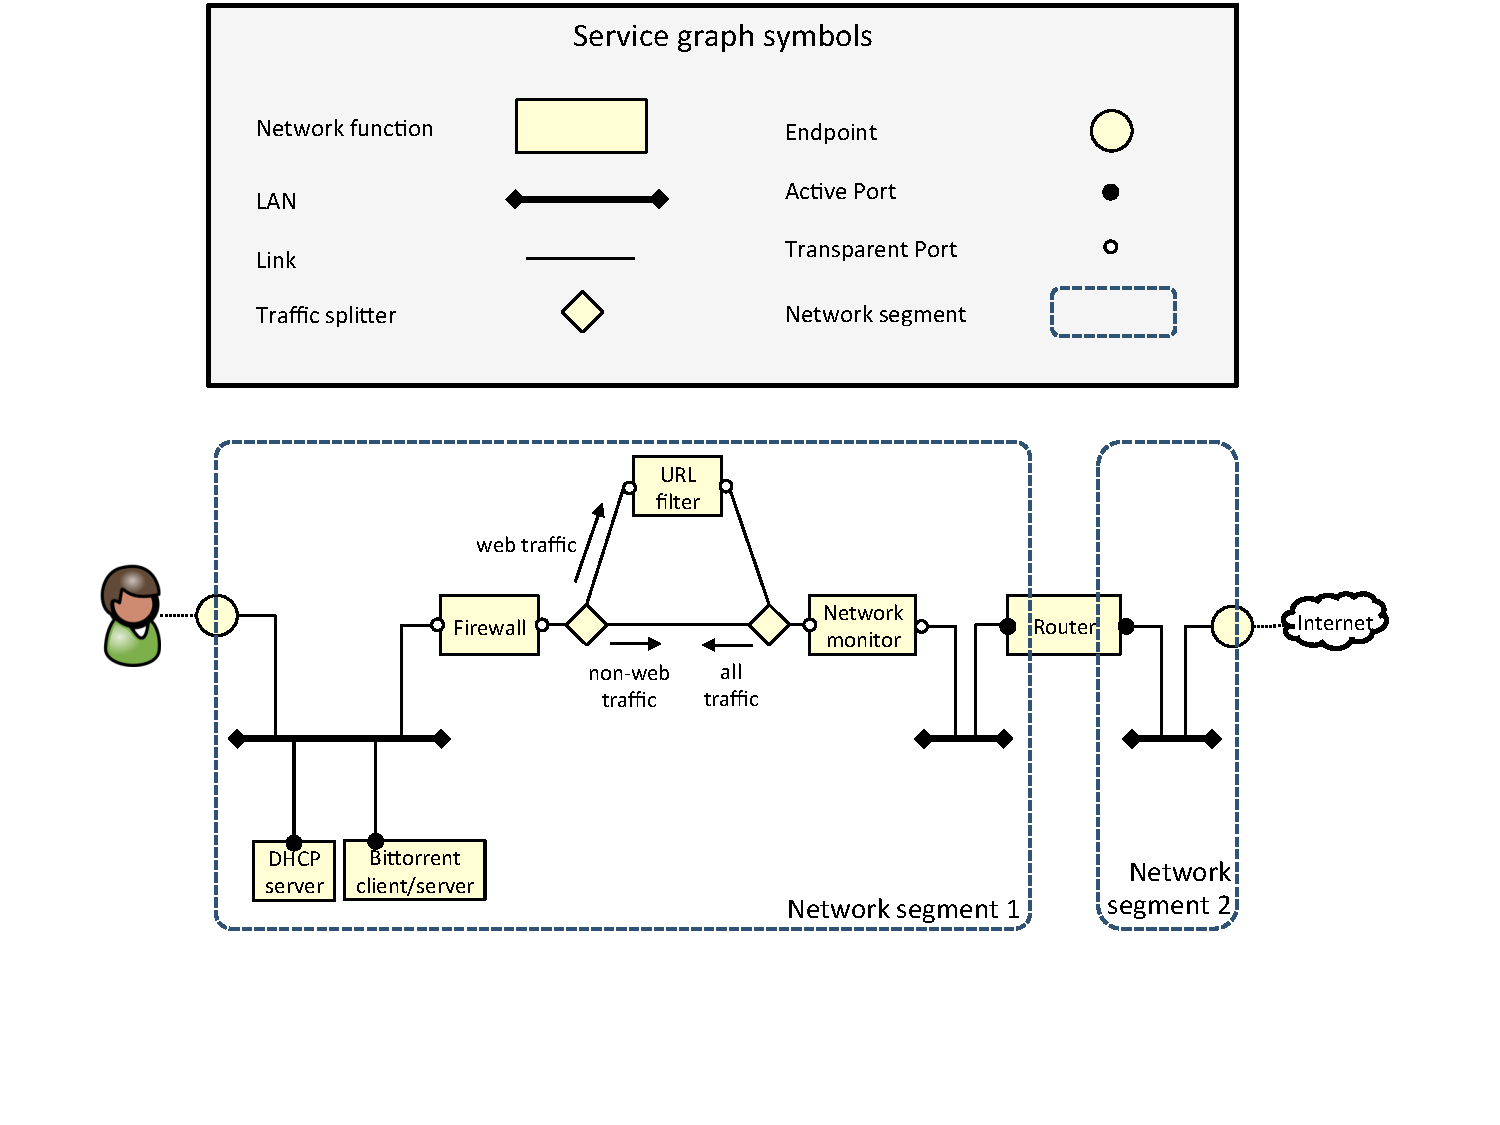
\includegraphics[clip= true, width= 0.8\columnwidth, trim= 1.5cm 3.0cm 0.6cm 0.0cm]{images/service_graph_components.pdf}
	\caption{Service graph: basic elements and example.}
	\label{fig:service_graph}
\end{figure}

From the point of view of the infrastructure, the SG consists of the set of basic elements shown in Figure~\ref{fig:service_graph}, which have been selected among the most common elements that we expect are needed to define network services.
In particular, a SG may include the following seven basic primitives:
\begin{itemize}
	\item \textbf{Network function}: it represents a functional block that may be lately translated into one (or more) VNF images. %, or to a dedicated hardware.
	%IVANO: ho rimosso il "to a dedicated hw". Perché secondo me è un dettaglio .
	%, without differentiating between transparent (e.g., network monitor) and ``active'' functions network whose network interfaces have with IP addresses, and hence that can be explicitly addressed by packets (e.g., a web server);
	Each network function is associated with a template (detailed in Section~\ref{sec:template}) describing the function itself in terms of RAM and CPU required, type of processor on which it can run (e.g., x86-64), number and types of ports, etc.
	\item \textbf{Active port}: it defines the attaching point of a network function that needs to be configured with a network-level address (e.g., IP), either dynamic or static. Packets directed to that port are forwarded by the infrastructure based on the link-layer address of the port itself (e.g., MAC address).
	\item \textbf{Transparent port}: it defines the attaching point of a network function whose associated virtual network interface card (vNIC) does not require any network-level address. If traffic has to be delivered to that port, the network infrastructure has to ``guide'' packets to it, e.g., through traffic steering elements, since the natural forwarding of the data based on link-layer addresses does not cross those ports.
	\item \textbf{Local area network (LAN)}: it represents the (logical) broadcast communication medium, i.e., the well-known primitive that allows data-link frames to be delivered to the correct recipient. The availability of this primitive facilitates the creation of complex services that include not only transparent VNFs, but also traditional host-based services that are usually designed in terms of LANs and hosts. Furthermore this provides an abstraction similar to the one available in cloud management systems, such as OpenStack, that usually offer the \textit{network} as one of the fundamental building blocks.
	\item \textbf{Point-to-point link}: it defines the logical wiring among the different components, and can be used to connect two VNFs together, 
	%implement the traffic steering between different network functions (e.g., when the output of VNF1 represents the input of VNF2), 
	to connect a port to a LAN, and more. %Links are accompanied by the proper attaching rules that define how they can be connected to the different components.
	\item \textbf{Traffic splitter/merger}: it represents a functional block that allows to split the traffic based on a given set of rules, or to merge the traffic coming from different links. For instance, it can be used to redirect only the outgoing web traffic toward an URL filter (Figure~\ref{fig:service_graph}), while the rest does not crosses that network function.
	\begin{comment}
	%IVANO: un endpoint non e' una porta fisica nel SG, così come non è un tunne gre. Poi, nel processo di lowering,  possono diventare tunnel gre o porte fisiche-
	\item \textbf{Endpoint}: it represents the external attaching point of the service graph, which can be a physical/logical port (e.g., a physical NIC, a virtual NIC or a network tunnel endpoint) or the endpoint of another service graph, if several of them have to be cascaded.
	\end{comment}
	\item \textbf{Endpoint}: it represents the external attaching point of the SG. It can be used to attach the SG to the Internet, to an end user device, but also to the endpoint of another service graph, if several of them have to be cascaded in order to create a more complex service.
	To this purpose, each endpoint is associated \textit{(i)} with an identifier, which can be used as a reference to connect two SGs together, and \textit{(ii)} with a cardinality, which indicates if the endpoint can be connected to one or many other endpoints.
\end{itemize}

In the example of SG provided in Figure~\ref{fig:service_graph}, three network functions are connected to a LAN, featuring both active (e.g., the DHCP server and the bittorrent machine, which need to be configured with IP addresses) and transparent ports (the firewall).
The outgoing traffic exiting from the firewall is received by a splitter/merge block, which redirects the web traffic to an URL filter and from here to a network monitor, while the non-web traffic travels directly from the firewall to the network monitor.
Finally, the entire traffic is sent to a router %(that originates two different network segments)
before exiting from the service graph.
It is worth noting that traffic splitter/merger modules are bidirectional and may have different behaviors in the opposite directions.
For instance, the traffic splitter/merger on the right will send \textit{all} the traffic coming from Internet to the firewall, without sending anything to the URL filter as this block needs to operate only on the outbound traffic.





As cited above, the SG also includes aspects related to the configuration of the network functions required by the service;
particularly, this information includes network aspects such as the IP addresses assigned to the active ports of the VNFs, as well as VNF-specific configurations, such as the filtering rules for a firewall.
In fact, they represent important service-layer parameters to be defined together with the service topology, %, although they are not needed to actually deploy the VNFs and virtual links in the network infrastructure.
and that can be used by the control/management plane of the network infrastructure to properly configure the service.

A SG engine may also assess formal properties on the above configuration parameters; for example, the service may  be analyzed %by some verification tools that 
to check if the IP address assigned to the VNFs active ports are coherent among each others.
To facilitate this work, the SG includes the concept of \textbf{network segment}. 
According to Figure~\ref{fig:service_graph}, each network segment is the set of LANs, links and ports that are either directly connected or that can be reached through a network function by traversing only its transparent ports. 
Hence, it corresponds to an extension of the broadcast domain, as in our case data-link frames can traverse also network functions (through their transparent ports), and it can be used to check that all the addresses (assigned to the active ports) of the same network segment belong to the same IP subnetwork.
As shown in the picture, a network segment can be extended outside of the SG; for instance, if no L3 device there exists between an end user terminal and the graph endpoint, the network segment also includes the user device.





As a final remark, the configuration parameters for the network functions, as well as the possibility of assessing formal properties on them, are out of the scope of this paper and will be investigated in our future work.
\begin{comment}


\section{Service graph}
%\chapter{Service graph}
\label{chap: Service graph}
\label{sec:service_graph}

In our topology of service we defined a model used to represent an high level of service that the user asks to the network, this is called Service graph. It consists of the set of basic elements shown in Figure \ref{fig:service_graph_components}. 
\begin{figure}[h]
	\centering
	% left bottom right top
	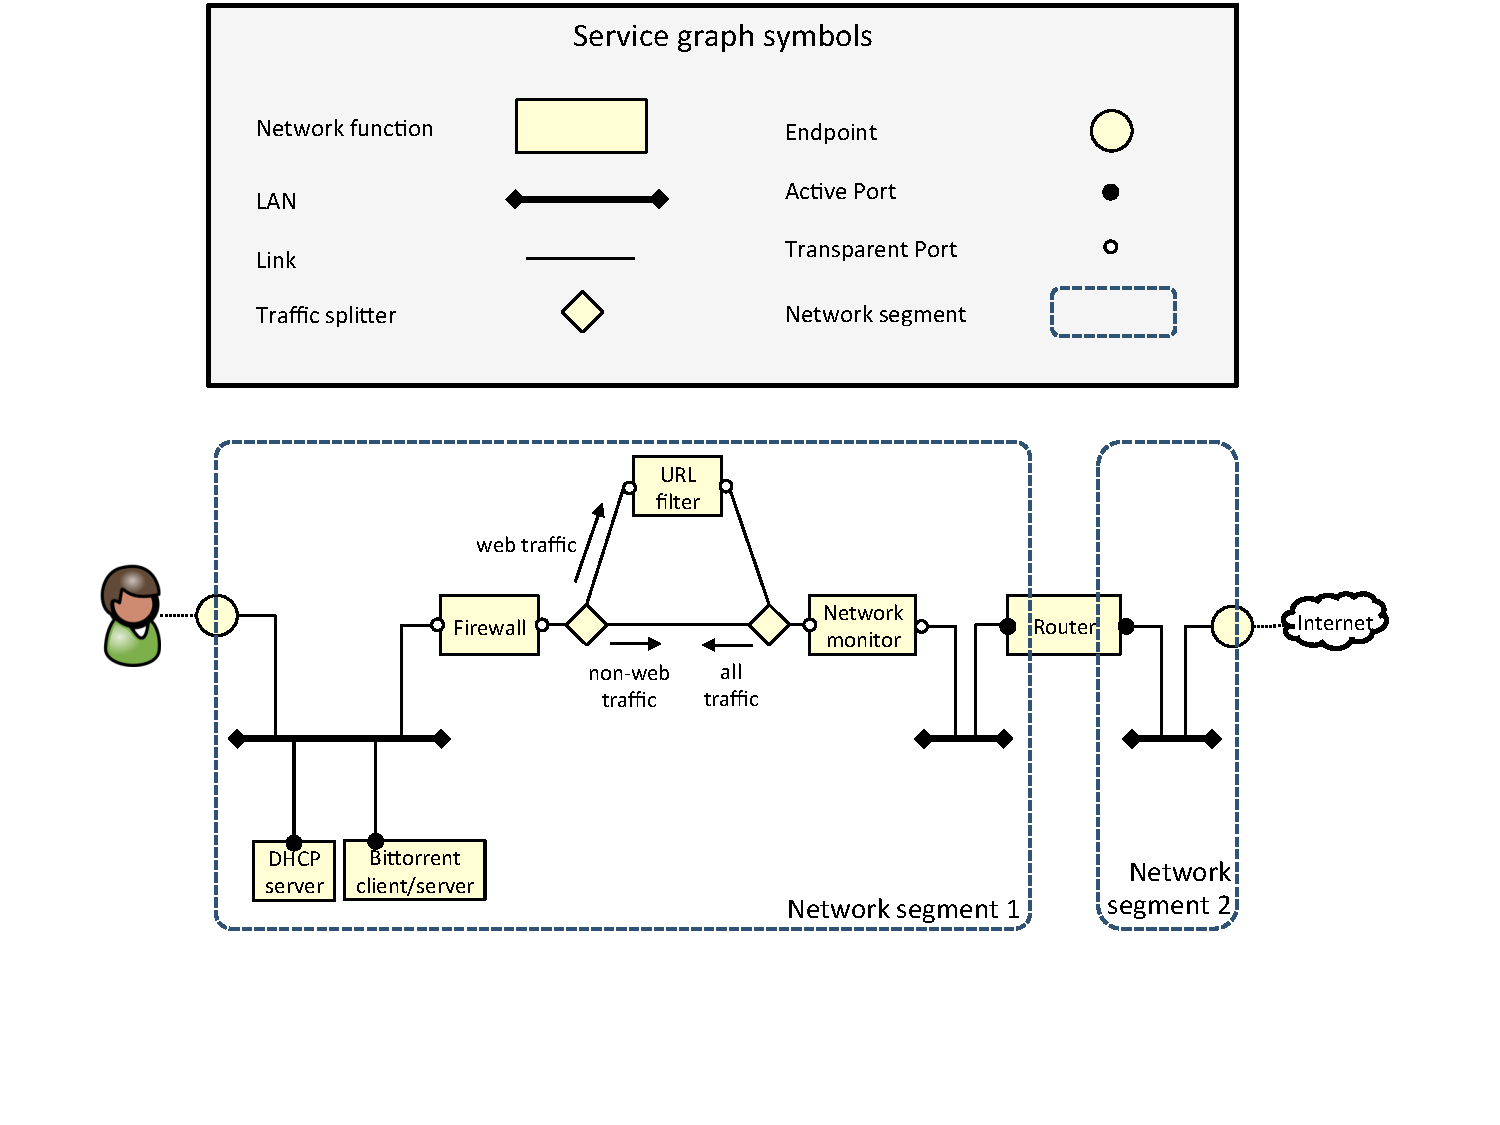
\includegraphics[clip= true, width= \columnwidth]{images/service_graph_components.pdf}
	\caption{SG - Service graph components}
	\label{fig:service_graph_components}
\end{figure}
These primitives have been selected among the most common elements that we expect are needed by the users to create their own network service.
In particular, a SG may include the following seven basic primitives:
\begin{itemize}
	
	\item \textbf{Network functions}: it represents a functional block that may be lately translated into one (or more) VNF images. It can arbitrarily create/delete packets, change the packet content (e.g., protocol headers/data), and determine the output port where to send it. The internal behavior of this functional block is not known by the other entities and it is arbitrarily determined by the service (e.g., network function) itself.
	
	\item \textbf{Active port}: it defines the attaching point of a network function that needs to be configured with a network-level address (e.g., IP), either dynamic or static. Packets
	directed to that port are forwarded by the infrastructure based on the link-layer address of the port itself (e.g., MAC address).
	
	\item \textbf{Transparent port}: it defines the attaching point of a network function whose associated virtual network interface card (vNIC) does not require any network-level address. If traffic has to be delivered to that port, the network infrastructure has to “guide” packets to it, e.g., through traffic steering elements, as the natural flow of data, which is based on link-layer addresses, does not cross those ports.
	
	\item \textbf{Local area network (LAN)}: it represents the (logical) broadcast communication medium, i.e., the well-known primitive that allows data-link frames to be delivered to the correct recipient. The availability of this primitive facilitates the creation of complex services, as network-savvy people still tend to think about networks and hosts.
	
	\item \textbf{Point-to-point link}: it defines the logical wiring among the different components. It can be used to implement the traffic steering between different network functions (e.g., when the output of VNF1 represents the input of VNF2), to connect an active port to a LAN, and more. Links are accompanied by the proper attaching rules that define how they can be connected to the different components.
	
	\item \textbf{Traffic splitter/merger}: it represents a functional block that allows to split the traffic based on a given set of rules, or to merge the traffic coming from different links. For instance, it can be used to redirect only the outgoing web traffic toward an URL filter (Figure 2), while the rest does not crosses that network function.
	
	\item \textbf{Endpoint}: it represents the external attaching point of the SG. It can be used to attach the SG to the Internet, to the user device, but also to the endpoint of another service graph, if several of them have to be cascaded.
	
\end{itemize}

Moreover, the SG can also include network-layer information such as IP address. In fact, although IP addresses are not needed at all when we need to deploy VNFs and virtual links in the network infrastructure, they may represent an important service-layer parameter for users, who may need to define them together with the service topology.
In the example of SG provided in Figure 2, three network functions are connected to a LAN, featuring both active (e.g., the DHCP server and the bittorrent machine, which need to be configured with IP addresses) and transparent ports (the firewall). The outgoing traffic exiting from the firewall is received by a splitter/merge blocks, which redirects the web traffic to an URL filter and from here to a network monitor, while the non-web traffic travels directly from the firewall to the network monitor. Finally, the entire traffic is sent to a router (that originates two different network segments) before exiting from the service graph.
It is worth noting that traffic splitter/merger modules are bidirectional and may have different behaviors in the opposite
directions. For instance, the traffic splitter/merger on the right will send all the traffic coming from Internet to the firewall, without sending anything to the URL filter as this block needs to operate only on the outbound traffic.
The required service, before being actually instantiated on the network, may need to be analyzed by some verification tools, which check if the SG satisfies some properties. To facilitate the work of these tools, we defined the network segment element, which is shown in Figure 2. As evident from the picture, each network segment is the set of LANs, links and ports that are either directly connected or that can be reached through a network function by traversing only its transparent ports. Hence, it corresponds to an extension of the broadcast domain, as in our case data-link frames can traverse also network functions (through their transparent ports), and it can be used to check that all the addresses (assigned to the active ports) of the same network segment belong to the same IP subnetwork. It is worth noting that the network segment may also include the user terminal, if no L3 device there exists between the terminal itself and the graph endpoint, as shown in the left of the picture.
As a final remark, in order to facilitate the service creation, we expect that the user is provided with a graphical interface that makes available the above elements (except the network segments, generated by the system), and that is integrated with an AppStore-like marketplace that enables uses to select a precise function among the many available.
\end{comment}

\subsection{Cascading service graphs}
\label{sec:ep_cascade}

As introduced above, the SG endpoints are associated with multiple parameters that are used to connect SGs together (cascading graphs). 
Particularly, the name is the foundation of the SG attaching rules, indeed  %as only the endpoints with the same identifier (shown with the same color in Figure ) can be attached together.
the logic that connects the endpoints is demanded to service layer but is done on the basis of their names.

The cardinality specifies if that endpoint can be used to connect the graph with one or many other graphs, i.e., to implement a one-to-one or a one-to-many connection. Finally, the optional ingress matching rule indicates which traffic is allowed to enter into the graph through that particular endpoint, e.g., only the packets with a specific source MAC address.

The cardinality specifies if that endpoint is used to connect the graph with one or many other graphs, i.e., to implement a one-to-one or a one-to-many connection. Finally, the optional ingress matching rule indicates which traffic is allowed to enter into the graph through that particular endpoint, e.g., only the packets with a specific source MAC address.

The rules that define how to connect several graphs together change according to both the cardinality of the endpoints involved and to the presence of an ingress matching rule on such endpoints. While the case in which only two endpoints have to be connected (i.e., direct connection) does not present significant issues, Figure~\ref{fig:endpoints} presents two examples in which an one-to-one endpoint (in the SG on the left) must be connected to a common graph through its one-to-many endpoint. In this example we consider a first packet flowing from the left to the right, while the return packet follows the opposite path.

\begin{figure} %[h]
	\centering
	% left bottom right top
	\includegraphics[clip= true, width= 0.9\columnwidth, trim= 0.1cm 1.2cm 0cm 0.0cm, page= 19]{images/Pictures_definitivo.pdf}
	\caption{Connection of many user SGs to a single ISP SG.}
	\label{fig:endpoints}
\end{figure}

Example 1 in Figure~\ref{fig:endpoints} presents two egress endpoints that are associated with a ingress matching rule specifying which traffic must enter into the graph through that endpoint. This ingress matching rule must be used, in case of return traffic, to deliver the desired packets to the correct graph, notably HTTP traffic to the “HTTP-SG” and FTP traffic to the “FTP-SG”. This is achieved by transforming the ingress endpoint of the “TCP-SG” into the set of components enclosed in the green shape of Example 1(b), notably a traffic splitter/merger module attached with many new endpoints, each one connected to a different graph. This way, the common “TCP-SG” will be able to dispatch the packet answers to the proper graph.
Example 2 in Figure 4 shows instead the case in which the egress endpoints are not associated with any ingress matching rule, which makes impossible to determine the right destination for the packets on the return path as a traffic splitter/merger module cannot be used in the “ISP-SG” to properly dispatch the traffic among them. In this case, the ingress endpoint of the common “ISP- SG” is transformed into a LAN connected to several new endpoints, each one with one-to-one cardinality and dedicated to the connection with a single other graph. This way, thanks to the MAC-based forwarding guaranteed by the LAN, the “ISP-SG” can dispatch the return packets to the proper graph, based on the MAC destination address of the packet itself.
%
%
%
%
\begin{comment}
The SG and FG models proposed in this thesis allow the concatenation of many service graphs through the graph endpoints.
To this purpose, each endpoint is associated with an unique identifier and a cardinality, indicating if that endpoint can be used to connect the graph with one or many other graphs, i.e., to implement a \texttt{one-to-one} or a \texttt{one-to-many} interconnection.
Then, before the FG is given to Infrastructure layer, the endpoints are manipulated as follows.
If the connection is between endpoint never connected until now (\texttt{one-to-one} connection) endpoints are let unmodified, while if at least one of endpoints evolved  in the connection are already connected with an other graph (\texttt{one-to-many} connection),  endpoint is connected with a LAN connected with several new endpoints, each one marked as \texttt{one-to-one}, and that will be dedicated to the connection to a single other graph.

To better understand, consider the use case under analysis, which requires that each end user SG is cascaded with a common graph defined by the ISP, so that: \textit{(i)} the packets generated by the end users are processed in the ISP graph before going towards the Internet; \textit{(ii)} the packets coming from the Internet are first handled by the ISP graph, which is then able to provide them to the proper user SG.
%Hence, the following of this section details how these inter-SG connections are implemented in our service layer, by using as an example our use case.

Particularly, referring to Figure~\ref{fig:endpoints}(a), the \textit{egress} endpoint of each user SG must be connected to the \textit{ingress} endpoint of the ISP SG.
As a consequence, the \textit{egress} endpoint of the user graph is marked as \texttt{one-to-one}, while the \textit{ingress} endpoint of the ISP graph is marked as \texttt{one-to-many}. %, since it must be connected to several end user graphs\footnote{Remember, in fact, that the ISP graph is shared among all the end users.}.
Hence, the service layer replaces this last endpoint with several new endpoints connected to a LAN, as depicted in Figure~\ref{fig:endpoints}(b).

\begin{figure} %[h]
	\centering
	% left bottom right top
	\includegraphics[clip= true, width= 0.9\columnwidth, trim= 0.1cm 1.2cm 0cm 0.0cm, page= 19]{images/Pictures_definitivo.pdf}
	\caption{Connection of many user SGs to a single ISP SG.}
	\label{fig:endpoints}
\end{figure}


According to Figure~\ref{fig:endpoints}(c), when a user SG is going to be deployed, its endpoint are not expanded, since they are marked as \texttt{one-to-one}.
However, the SLApp creates a logical connection between the \textit{egress} endpoint of the graph itself and one of the new endpoints of the ISP SG.
This way, the orchestration layer (which has no information on the use case implemented by the service layer) knows that the traffic going towards/coming from the Internet must be processed by the ISP SG after/before going towards its final destination, %and that traffic coming from the Internet must enter in the ISP SG before being handled by the service defined by a specific user, 
and hence can instruct the infrastructure layer to create the proper links.


\end{comment}


\section{Forwarding graph}
\label{sec:forwarding_graph}

The SG provides an high level formalism to define network services, but it is not adequate to be deployed on the physical infrastructure of the network, since it does not include all the details that are needed by the service to operate.
Hence, it must be translated into a more resource oriented representation, namely the \textbf{forwarding graph (FG)} (Chapter~\ref{chap:the_state_of_the_art}), through the so called \textbf{lowering process}.

The differences between the SG and the FG, together with the steps needed to transform a the first representation into the second one (i.e., the lowering process), are shown in Figure~\ref{fig:graphs} and discussed in the following:


\begin{figure}[h]
	\centering
	% left bottom right top
	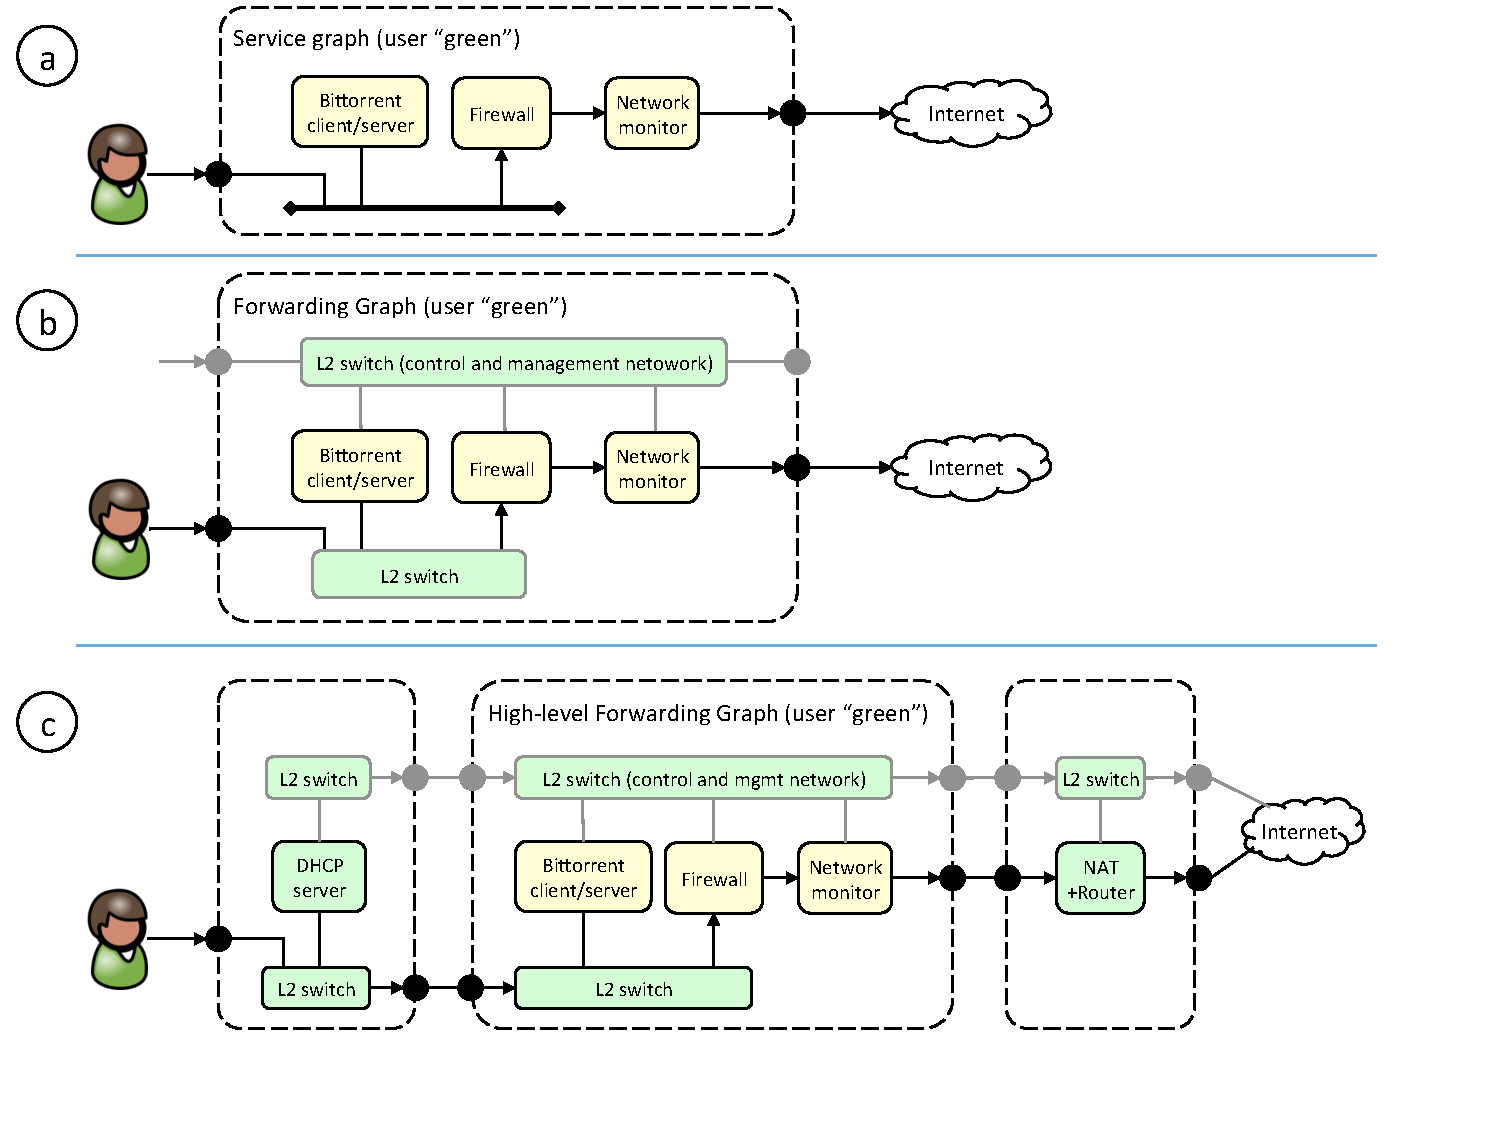
\includegraphics[clip= true, width= 0.8\columnwidth, trim= 0.0cm 1.4cm 1.2cm 0.0cm]{images/NF-FG.pdf}
	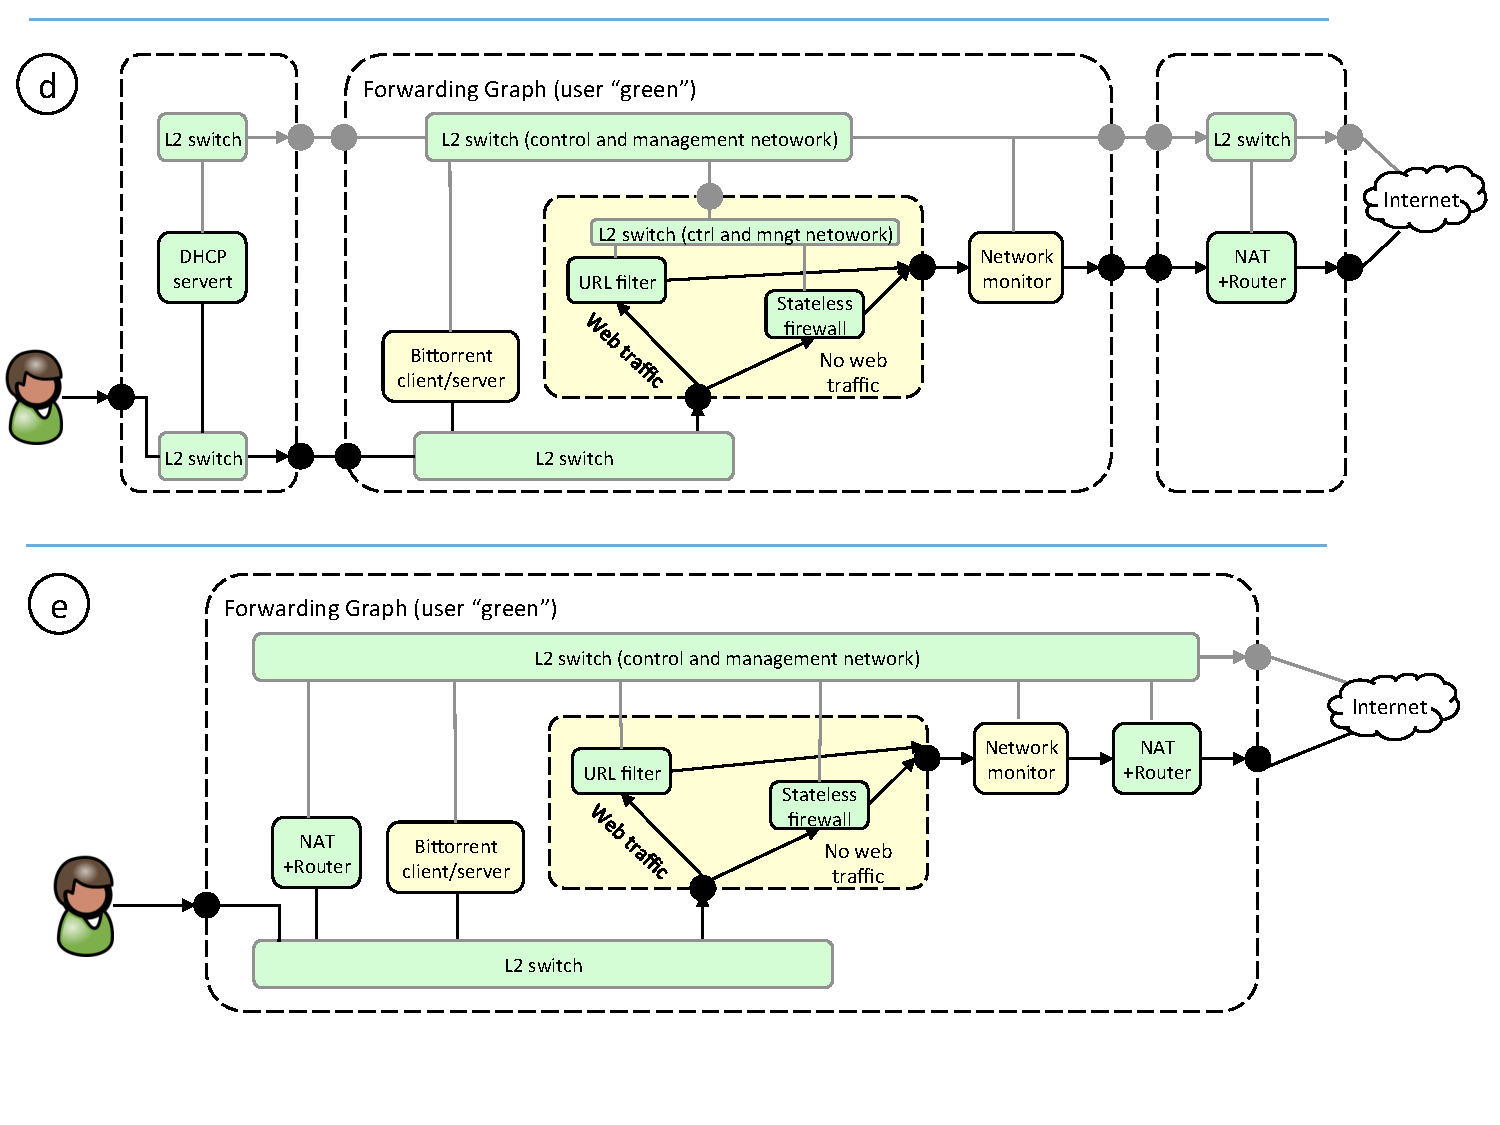
\includegraphics[clip= true, width= 0.8\columnwidth, trim= 0cm 1.8cm 0.2cm 0.0cm]{images/NF-FG2.pdf}
	\caption{From the service graph to the forwarding graph: the lowering process.}
	\label{fig:network_function_forwarding_graph}
	\label{fig:graphs}
\end{figure}

%
\begin{itemize}
	\item  \textbf{Control and management network expansion}: the service is enriched with the ``control and management network'', which may be used %only be accessible by some actors (e.g., the network provider) in order 
	to  properly configure  the VNFs of the graph.
	In fact, most network functions require a specific vNIC dedicated to the control/management operations; although this may be an unnecessary detail for the user requiring the service, those network connections have to be present in order to allow the service to operate properly. 
	An example of this step is evident by a comparison between Figure~\ref{fig:graphs}(a) and  Figure~\ref{fig:graphs}(b), in which a control/management network consisting of a L2 switch VNF has been added to the graph\footnote{It is worth pointing out that, although the control and management network in Figure~\ref{fig:graphs}(b) only includes a L2 switch, this network could also include other VNFs, such as a firewall.}.
	\item \textbf{LAN expansion}: all the LANs expressed in the SG are replaced with VNFs implementing the MAC learning switch.
	This step is again shown in Figure~\ref{fig:graphs}(b), and it is needed in order to translate the abstract LAN element available in the SG into a VNF actually realizing the broadcast communication medium.
	\item \textbf{Service enrichment}: the graph is analyzed and enriched with those functions that have not been inserted in the SG, but that are required for the correct implementation and delivery of the service.
	As shown in the example provided in Figure~\ref{fig:graphs}(c), if the graph analysis determines, for instance, that the graph does not include a DHCP server and does not terminate with a VNF acting as a router and as a NAT,  these functions are automatically added at this step of the lowering process.
	\item \textbf{VNFs expansion}: according to its template described in Section~\ref{sec:template}, a VNF may be expanded in a number of VNFs, properly connected in a way to implement the required service.
	As an example, the firewall in Figure~\ref{fig:graphs}(c) is replaced, in Figure~\ref{fig:graphs}(d), with a subgraph composed of an URL filter only operating on the web traffic, while the non-web traffic is delivered to a stateless firewall.
	As evident, the ports of the ``original'' VNF are now the endpoints of the new subgraph, which also have a control network dedicated to the new VNFs.
	Moreover, these new VNFs are in turn associated with a template, and can be recursively expanded in further subgraphs; this is an implementation of the ``\textit{recursive functional blocks}'' concept provided by NFV definition in ETSI standard (Chapter~\ref{chap:the_state_of_the_art}).
	\item \textbf{Consolidation}: it consists in the replacement, with a single VNF, of those VNFs implementing the L2 forwarding that are connected together, in order to limit the resources required to implement the LANs on the physical infrastructure.
	An example of this step is provided in Figure~\ref{fig:graphs}(e).
	\item \textbf{Endpoint translation}: it is the last step of the lowering process, in which the graph endpoints can be converted in: physical ports of the node on which the graph will be deployed; tunnel endpoints (e.g., GRE) used to connect two pieces of the same service but on different physical servers; endpoints of another FG, if many graphs must be connected together in order to create a more complex service.
	\item Finally, the \textbf{flowrules definition} concludes the lowering process. In particular the connections among the VNFs, as well as the traffic steering rules (expressed through the traffic splitter/merger components in the SG) can be represented with a sequence of ``flowrules'' (Listing~\ref{lst:NF-FG_flowrule}), each one indicating which traffic has to be delivered to a specific VNF (on a given port of that VNF), or the physical port/endpoint through which the traffic has to leave the graph. 
	
	\lstinputlisting[label=lst:NF-FG_flowrule, language=python, caption={Example of flourule associated to specific VNF port.}]{code/NF-FG_example_vnf_flowrules.txt}
	
	
	The flowspec supports all the fields defined by Openflow 1.0~\cite{of10} (although new fields can be defined), while the action can refer to a forwarding of packets either through a physical port, through a logical endpoint, or through a port of a VNF. 
	Hence, the FG is actually a generalization of the Openflow data model that specifies also the functions that have to process the traffic into the node, in addition to define the (virtual) ports the traffic has to be sent to.
	
	
	
\end{itemize}










\begin{comment}


\section{Forwarding graph}
\label{sec:forwarding_graph}

\begin{figure}[h]
	\centering
	% left bottom right top
	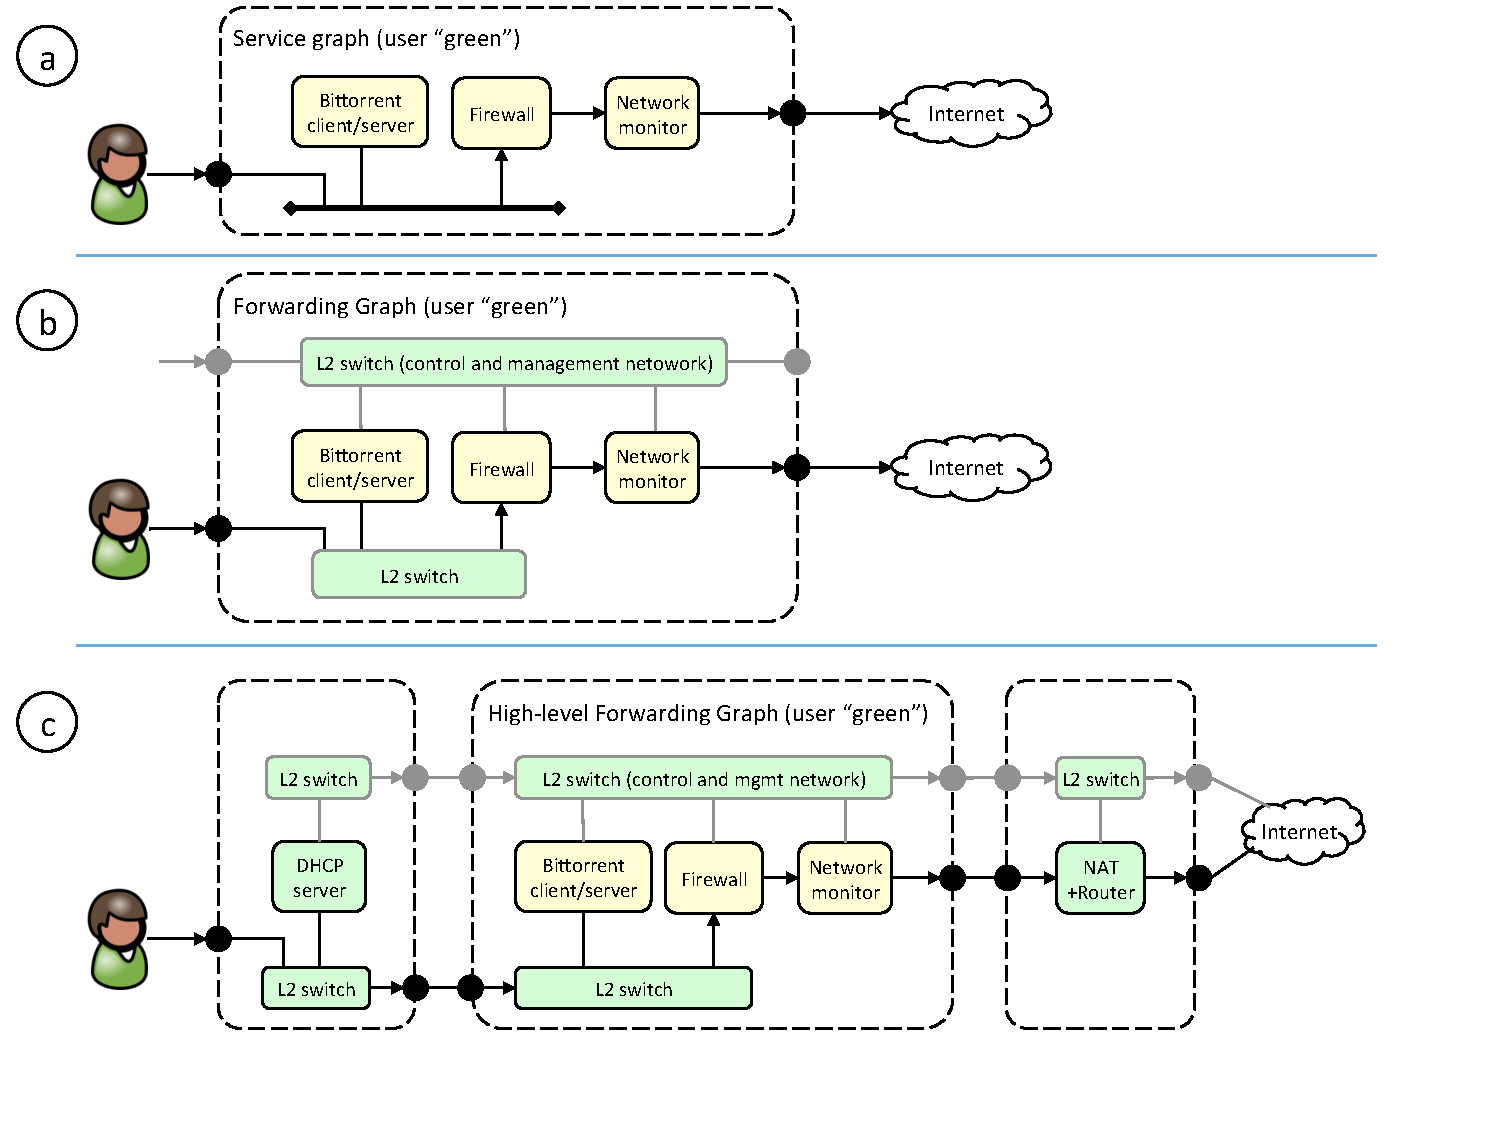
\includegraphics[clip= true, width= 0.8\columnwidth, trim= 0.0cm 1.4cm 1.2cm 0.0cm]{images/NF-FG.pdf}
	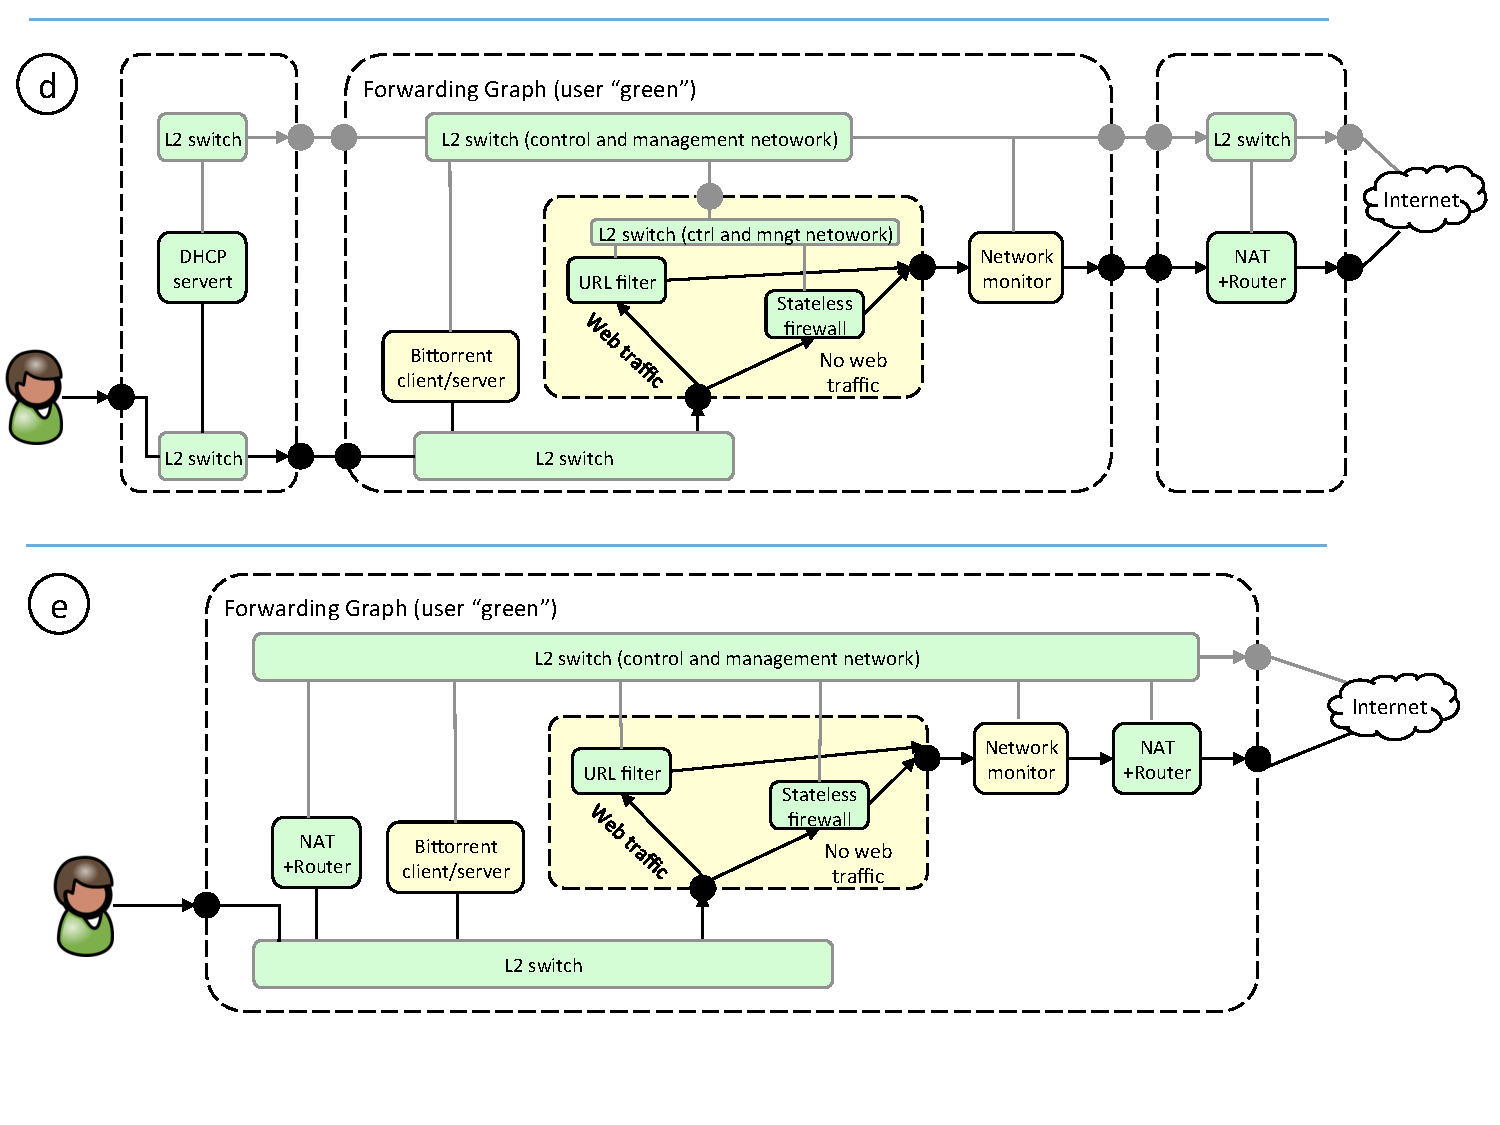
\includegraphics[clip= true, width= 0.8\columnwidth, trim= 0cm 1.8cm 0.2cm 0.0cm]{images/NF-FG2.pdf}
	\caption{From the service graph to the forwarding graph: the lowering process.}
	\label{fig:network_function_forwarding_graph}
	\label{fig:graphs}
\end{figure}

The SG just introduced provides to the users an high level formalism to define their services, but it is not adequate to be deployed on the physical infrastructure of the network. Hence, it must be lowered into a more resource oriented representation, namely the \textbf{forwarding graph (FG)}. Although, similar to the SG, this formalism provides an end-to-end description of the VNFs involved in the service itself and their logical connections, the SG does not include all the details that are needed by the service to operate, and hence several differences there exist between the two representations. These differences, together with the steps needed to transform a SG into a FG (i.e., to implement the \textbf{lowering process}) are shown in Figure \ref{fig:network_function_forwarding_graph} and discussed in the following of this section.
First of all, most network functions require a specific vNIC dedicated to the control/management operations, which may be accessible only by the network provider. Although this is an unnecessary detail for the user, those network connections have to be present in order to allow the service to operate properly. Hence, the first step of the logic that translates the SG into the actual building blocks has to complete the FG with the control and management network, as evident by a comparison between Figure \ref{fig:network_function_forwarding_graph}(a) and Figure \ref{fig:network_function_forwarding_graph}(b).The latter picture also shows the second step of the lowering process, which consists in the replacement of the LANs expressed in the SG with VNFs implementing the MAC learning switch, called “L2 switch” in the figure.
Figure \ref{fig:network_function_forwarding_graph}(c) shows instead the third step of the process to translate the SG into a FG, which consists in the enrichment of the service expressed by the user with a number of VNFs needed for the correct implementation of the service itself. For example, the picture shows that the user graph is connected to the left with a first graph containing a DHCP server attached to a switch, while to the right it is connected with a second graph that consists of a VNF implementing a router and a NAT. The SG considers a network function like a generic functional block, hence missing low-level details such as the number (and types) of software images that need to be instantiated. For instance, a VNF expressed in the SG may be expanded in a number of VNFs in the FG, properly connected in a way to implement the required service: this is the fourth step of the lowering process. As an example, the firewall in the Figure \ref{fig:network_function_forwarding_graph}(c) is replaced, in Figure \ref{fig:network_function_forwarding_graph}(d), with a subgraph composed of an URL filter only operating on the web traffic, while the non-web traffic is provided to a stateless firewall. It is worth noting that the ports of the “original” VNF are now the endpoints of the new subgraph, which also have a control network dedicated to the new VNFs.
Finally, the last step of the lowering process consists in the consolidation of the three pieces of graph into a single one, as shown in Figure \ref{fig:network_function_forwarding_graph}(e). In this step, the VNFs implementing the L2 forwarding and that are connected together are replaced with a single VNF, in order to limit the resources required to implement the LANs on the physical infrastructure.


\lstinputlisting[label=lst:NF-FG_flowrule, language=python, caption={Example of flourule associated to specific VNF's port}]{code/NF-FG_example_vnf_flowrules.txt}


In addition, all the connections among the VNFs and the traffic steering rules (expressed through the traffic splitter/merger components in the SG) originate a sequence of “flowrules” associated to each VNFs port (Listing \ref{lst:NF-FG_flowrule}), each one indicating which traffic has to be delivered to a specific VNF (on a given port of that VNF), or the endpoint through which the traffic has to leave the graph. The action can refer either to an endpoint or to a port of a VNF, while the matches in flow spec supports all the fields defined by Openflow 1.0 (although new fields can be defined). In this respect, we can consider the FG as a generalization of the Openflow data model that specifies also the functions that have to process the traffic into the node, in addition to defining the (virtual) ports the traffic has to be sent to.
Furthermore in the current implementation of FG the labels associated in the SG to endpoints shown in Figure~\ref{fig:endpoints} become ingoing rules for the VNFs ports linked to the endpoints.

As a final remark, the FG does not specify yet low level details such as the physical node on which the service will be deployed, as well as the reference to the precise physical/virtual interfaces needed by the VNF to operate, replaced by generic entry/exit points for the graph.
\end{comment}

\subsection{Structure of the FG}
This section contains a detailed analysis of the forwarding graph description.

The notation used to describe the forwarding graph is JSON (JavaScript Object Notation). A first level description of FG is given by Listing \ref{lst:NF-FG_example}.

\lstinputlisting[label=lst:NF-FG_example, language=python, caption={High-level view of FG.}]{code/NF-FG_example.txt}

The information contained in FG is: \textit{(i)} a list of virtual network functions, \textit{(ii)} a list of endpoints, \textit{(iii)} a unique identifier of the FG.
With regards to VNFs as shown in Listing \ref{lst:NF-FG_example_vnf}, they are characterized by a \texttt{vnf\_descriptor}, a list of \texttt{ports}, a \texttt{name} and an \texttt{id}.
\lstinputlisting[label=lst:NF-FG_example_vnf, language=python, caption={High-level view of VNFs.}]{code/NF-FG_example_vnf.txt}

% Ports

The ports described in VNFs JSON object are the ports actually used by a VNF, while a complete list of ports available for a VNF is contained in the VNF template (Section \ref{chap:VNFdescriptor}). Now we are going to analyze each field of the \texttt{VNFs} element in detail.

The \texttt{id} is an unique identifier of the VNF in the FG, while the \texttt{name} identify the type of VNF.
The \texttt{vnf\_descriptor} is an URL containings a manifest of the virtual network function that are (described in section \ref{chap:VNFdescriptor}).
The \texttt{port} list that are shown in the Listing \ref{lst:NF-FG_example_vnf_ports} contains an \texttt{id}, an \texttt{ingoing\_label}, and an \texttt{outgoing\_label}.
The port \texttt{id} is composed of two different parts, the part before the column identify the label (this one will be explained in section \ref{chap:VNFdescriptor}) of the port, the second part is an id for all ports with same label.  The \texttt{outgoing\_label} contains flow rules that only identify outgoing traffic from the port, while \texttt{ingoing\_label} contains flow rules only for ingoing traffic to that port.
While the outgoing labels are mandatory, the ingoing labels is needed only when a port is connected to an endpoint, since the endpoint does not have any flowrule associated.
In addiction, flow rules contained in an ingoing label have an addictional field to identify the endpoint from which the traffic comes. This field is called \texttt{ingress\_endpoint} and it is a leaf of flowspec object (line 10 of Listing~\ref{lst:NF-FG_flowrule}). Finally the flowrule object, as discussed before (Listing~\ref{lst:NF-FG_flowrule}) contains a list of matches on packets and the relative action. 


\lstinputlisting[label=lst:NF-FG_example_vnf_ports, language=python, caption={High-level view of ports}]{code/NF-FG_example_vnf_ports.txt}

It is worth noting that all the flow rules of a single port must forward the totality of traffic, hence, a rules of specific port cannot purge the traffic, and if we want to drop some kind of traffic we must do that in a VNF. Therefore it is clear that, the only type of actions can be ``output''.

% Endpoint

The \texttt{endpoints} (Listing~\ref{lst:NF-FG_example}) are the termination of graph. In the FG instead of SG, the endpoints can assume various characterizations like for example: \textit{(i)} tunnel termination, \textit{(ii)} physical port or \textit{(iii)} virtual port. For instance, the example in Listing \ref{lst:endpoint} shows an endpoint that is actually a physical port called "ge0". This characterization is needed to effectively connect graphs among each other and map the endpoint concept on physical resources.
\lstinputlisting[label=lst:endpoint, language=python, caption={NF-FG - Example of endpoint definition.}]{code/endpoint.txt}

With regard to name, it provides a tool to implement the logic of connection between graphs, together with a further field called \texttt{connection\_cardinality}, which specify the type of connection. It can assume two different values: \texttt{(i)} \texttt{one-to-many} or \texttt{(ii)} \texttt{many-to-many} as specified in Section~\ref{sec:ep_cascade}.
%that is present only when we should connect more than one endpoint to this endpoint. It consist of an id of a layer 2 switch VNF that are connected to this endpoint, the switch is used to route the packet in the right way. Therefore in this case the really endpoints (where the other graphs are really connected) are attached to other ports of the layer 2 switch link in figure \ref{}. This when necessary, is added by the service layer \ref{}.













\subsection{Operations}
As stated above, several actions can be executed on a FG. Particularly, these actions are: \textit{(i)} endpoint connection like in the passage between Figure \ref{fig:network_function_forwarding_graph}(d) and Figure \ref{fig:network_function_forwarding_graph}(e)  and \textit{(ii)} the node expansion like in the passage between Figure \ref{fig:network_function_forwarding_graph}(c) and Figure \ref{fig:network_function_forwarding_graph}(d).

\subsubsection{Connection}
The connection between different graphs is made through the endpoints, which represent the ingress/exit point from the graph. The connection depends on the service layer application implementation, indeed there are two possible types of connections: \textit{(i)} the graphs are logically connected, so the output of this operation is a new graph that doesn't have anymore the endpoints used for the connection, or \textit{(ii)} the connection operation preserve the endpoints used for the connection, so they can be used again for an other connection. The former case is evident by comparing  Figure~\ref{fig:network_function_forwarding_graph}(d) and Figure~\ref{fig:network_function_forwarding_graph}(e), while the latter case represents the situation in which the results of the operation are in turn two different graphs 
that communicate with each other through the endpoint (e.g. user graph connected to an ISP graph).
\begin{comment} 
\fabio{This connection is different depending on two possible situation: (i) the graphs should be logically connected (the union of these graphs represents only one graph belonging to single owner), (ii) the graphs should be connected and instantiated on the same host  or on different hosts (the union of these graph represent however two graphs belonging to two different owner). In the first case the connection is only logically and visible only at orchestration level and at the end of this operation the endpoint disappear, instead in the second case the connection is performed between graphs of two different users, this time it is a real connection and the endpoint must be characterized. }
\end{comment}
%
%
The connection process requires Cartesian product of the ingoing labels of ports directly connected to the endpoints involved in the operation of one graph and the outgoing label of specular ports on the other graph. In this way problem can arise in the resulting flows (especially with regard to the priorities, seen that we use Openflow in our implementation).

\paragraph{The flow rule merging problem}
\label{chap:the_merging_problem}

Endpoints connection has a problem merging the flowrules. Analyzing the problem, only the intersection between flow rules should remain after the connection of two endpoints, so when we try to connect two ports that were connected to two endpoints, if the intersection of the outgoing rules towards the endpoint of one and the ingoing rules from the endpoint of the other is null, then this two ports shouldn't be connected. To better explain this problem, consider the example shown in Figure \ref{fig:NF-FG_the_merging_problem}.
\begin{figure}[h]
	\centering
	% left bottom right top
	\includegraphics[clip= true, width= \columnwidth, trim= 0cm 2cm 0cm 0cm, page= 37]{images/Pictures_definitivo.pdf}
	\caption{The merging problem.}
	\label{fig:NF-FG_the_merging_problem}
\end{figure}
As evident the connection between VNF3 and VNF1 should disappear since there are not traffic matches in common. Furthermore, the traffic from VNF4 to VNF2 becomes the intersection between the totality of traffic (*) (prensent on the rule that bring the traffic from VNF4 to endpoint)  and the totality of traffic less tcp traffic on port 80 (*-TCP80) (prensent on the rule that bring the traffic from endpoint to VNF2), that is *-TCP80. 


\begin{figure}[h]
	\centering
	% left bottom right top
	\includegraphics[clip= true, width= \columnwidth, trim= 0cm 0.2cm 0cm 0cm, page= 38]{images/Pictures_definitivo.pdf}
	\includegraphics[clip= true, width= \columnwidth, trim= 0cm 10cm 0cm 0.2cm, page= 39]{images/Pictures_definitivo.pdf}
	\caption{NF-FG - The merging problem.}
	\label{fig:NF-FG_the_merging_problem_2}
\end{figure}


The biggest problem related to the fusion of rules is to assign the right priority to the traffic. In our formalism is not possible to express the rule \textit{all traffic \textbf{except} tcp traffic on port 80}. To better understand consider the high part of Figure~\ref{fig:NF-FG_the_merging_problem_2} where the following rules are expressed on a port of VNF3: one that brings traffic to VNF5 that has matches all TCP traffic on port 80, and having a certain priority, and the other rule for traffic to the endpoint  which matches all the traffic having a lower priority than the other. Hence, the priorities of the rules play a fundamental role in the actual construction of the network topology, and allow to realize the rule ``all traffic less''.
In the example shown in Figure~\ref{fig:NF-FG_the_merging_problem_2}, are included the  priority. As we can see from the ``FG final 1'' of Figure~\ref{fig:NF-FG_the_merging_problem_2}, assigning to flow rules on the port of VNF1 the priority of the flow rules of ``FG one'' the flow towards VNF5 is never used because it more specific than the other and have the lowest priority. Furthermore using, for all pair of flows generated from the connection, the priority of starting FG we will have the same priority to multiple rules. In this case, is not guaranteed the direction of flow (``FG final 2'' in the bottom right of Figure~\ref{fig:NF-FG_the_merging_problem_2}). Hence the right choice is more complicated of the simple copy of priority and in certain cases we should change accordingly a lot of rules (``FG final 3'' in the bottom of Figure~\ref{fig:NF-FG_the_merging_problem_2}). For these reasons and because this is not the core of the thesis the code implemented has the limitation of handle
only \textit{1 to 1} or \textit{1 to n} rules fusion, so the case \textit{n to n} like for VNF3 in Figure~\ref{fig:NF-FG_the_merging_problem_2} is not taken into account.

\subsubsection{Expansion of a VNF}
The terms VNF expansion means to replace a VNF with a new graph, in which the endpoints of the graph  correspond to the ports of the original VNF. For instance, looking at Figure~\ref{fig:network_function_forwarding_graph}(c), we can see that the firewall with three ports is replaced with a graph having three endpoints in figure 6.3(d).
\begin{comment}
\fabio{The expansion of a VNF occurs when downloading the image of VNF, thanks to the information contained in the vnf descriptor, we find an other forwarding graph instead of the really implementation of VNF (virtual machine or docker). }
\end{comment}
%
Furthermore is, possible to have a recursive expansion, for example, the firewall VNF of Figure~\ref{fig:firewall_expansion}(a) can be expansed like in Figure \ref{fig:firewall_expansion}{(b)} where there is a VNF named load balancer. This VNF, in turn,  is expanded in two functions, an openflow switch and an openflow controller that permits, with a proper logic in the openflow controller, to operate the switch as a load balancer.

\begin{figure}[h]
	\centering
	% left bottom right top
	\includegraphics[clip= true, width= 0.8\columnwidth, trim= 0cm 0cm 0cm 0cm, page=42]{images/Pictures_definitivo.pdf}
	\caption{Recursive VNF explosion.}
	\label{fig:firewall_expansion}
\end{figure}

Substantially, the expansion operation of a VNF may be reduced to a sequence of connection operations between logical graphs. In fact, once the VNF is replaced with the new graph, it is performed a connection of the endpoints of the new graph with endpoints born by cutting the links of the VNF expanded. Obviously, the rules associated with the ports of the old VNF are now associated at the ports of the boundary VNFs of new graph.









\section{Infrastructure graph}

\label{sec:ig}

The \textbf{infrastructure graph (IG)} is a further representation of the service to be deployed, which is semantical, but not syntactical, equivalent to the FG.
In fact, it consists of the sequence of commands to be executed on the physical infrastructure in oder to properly deploy the required VNFs and to create the paths among them.

The IG is obtained through the so called \textbf{reconciliation process}, which is described in the following of this section and consists in the mapping of the FG description (Section~\ref{sec:forwarding_graph}) on the resources available on the infrastructure.

\begin{comment}
In order to be deployed on the physical infrastructure, the FG described so far must be mapped on the resources (both physical and software) available on the node(s) on which the service is going to be instantiated.
This new representation of the service is called \textbf{infrastructure graph (IG)}, and it is obtained through the so called \textit{reconciliation} process.
More in detail, the reconciliation includes the transformations described in the following.
\end{comment}

First, some of the VNFs in the FG could be mapped on some modules (both software and hardware) available on the node on which the graph is going to be deployed, instead of being implemented with the specific image indicated in the template.
For example, if the node is equipped with a virtual switch (vSwitch) implementing the MAC learning algorithm (right part of Figure~\ref{fig:infrastructure_graph}), the L2 switch VNFs in the FG are removed, and their functionalities are mapped on the vSwitch itself.
Instead,  as depicted in the left of Figure~\ref{fig:infrastructure_graph}, if the node is equipped with a pure Openflow vSwitch, all the VNFs specified in the FG will be implemented through the proper images.
Obviously, other mappings between the VNFs and the resources available on the node are possible, according to the specific implementation of the infrastructure layer.
This translation is another implementation of the ``\textit{recursive functional blocks}'' concept~\cite{nfv}; in fact, starting from the same FG,  it will produce a different number of deployed VNFs according to the capabilities (e.g. L2 switching native support) of the node actually hosting the service.


\begin{comment}
In particular, an endpoint may need to be translated into a physical port, but it could also be converted into an entry point of another graph, since many SGs may need to be connected together.
%the service graph defined by the user must be connected to the service graph of another entity (e.g., the Internet Service Provider). 
For example, in Figure~\ref{fig:service_graphs}, the three SGs on the left will have one endpoint translated into the wireless physical interface of the node in which they will be deployed (e.g., \texttt{wlan0}), while the other endpoint will be connected with the graph on the right of the picture.
Moreover, in case a SG cannot be entirely deployed on the same node, it is split in several NF-FG to be deployed on different nodes and properly connected to implement the service required by the SG.
\end{comment}

\begin{figure}%[h]
	\centering
	% left bottom right top
	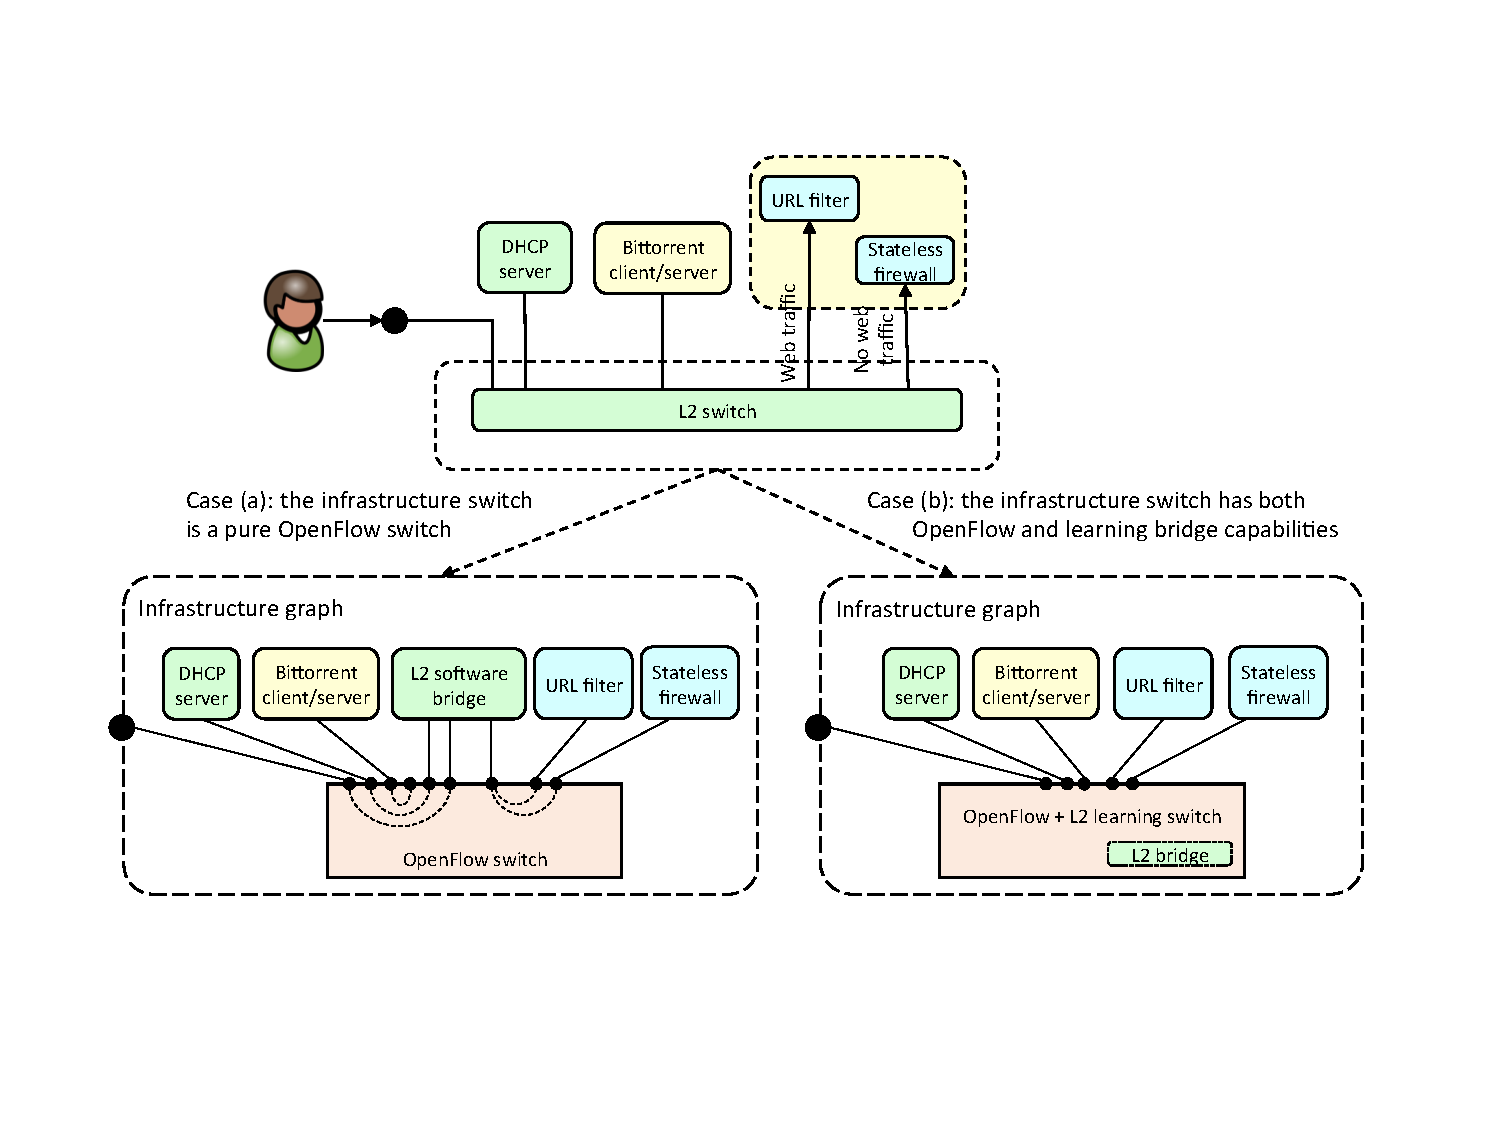
\includegraphics[clip= true, width= 0.8\columnwidth, trim= 0in 1.5in 0in 0in]{images/NF-FG_reconciliation.pdf}
	\caption{Part of the reconciliation process.}
	\label{fig:infrastructure_graph}
\end{figure}

Second, the flow rules defining the links of the FG, i.e., the connections among the VNFs, are properly translated according to the technology used by the physical node to implement the graph.
For example, if the physical node interconnects the VNFs through an Openflow vSwitch, each flow rule is converted in a number of Openflow \texttt{flowmod} messages.
However, other implementations of the infrastructure layer could implement these connections through other technologies, such as GRE tunnels or VLAN tags.

Similarly, each VNF is converted in the commands required to retrieve the image and start it up; also in this case, these commands depend on the technology implementing the VNFs (e.g., virtual machine, Docker containers, etc.).







\section{VNF template}
\label{chap:VNFdescriptor}
\label{sec:template}
As introduced above, each network function is associated with a template, which describes the VNF itself both in terms of infrastructure and in terms of configuration; an example of such a template is provided in Listing \ref{lst:NF-FG_templete}.

\lstinputlisting[label=lst:NF-FG_templete, language=python, caption={NF-FG - VNF template.}]{code/template2.txt}

As evident from listing example, the template contains some information related to the hardware required by the VNF, namely the amount of memory and CPU, as well as the architecture of the physical machine that can execute it and the requirements of disk in terms of swap, root file system and ephemeral file system size. Moreover, the boolean element \texttt{expandable} indicates if the VNF consists of a single image, or if it is actually a subgraph composed of several VNFs connected together. In the former case, the \texttt{uri} element refers to the image of the VNF, while in the latter it refers to a graph description, which must replace the original VNF in the forwarding graph. In case of non-expandable VNF, the template also specifies the type of the image; for instance, the firewall described in Listing \ref{lst:NF-FG_templete} is implemented as a single virtual machine.
Moreover, the template provides a description of the ports of the VNF, each one associated with several parameters. In particular, the label specifies the purpose of that port, and it is useful in the definition of the SG, since it helps to properly connect the VNF with the other components of the service (e.g., the external port of the firewall should be connected towards the Internet, while the internal ones should be connected towards the users). The label could assume any value, and it is meaningful only in the context of the VNF. The parameter \texttt{ipv4-config}, instead, indicates if the port cannot be associated with an IPv4 address (none), or if it can be statically (static) or dynamically (DHCP) configured, the same applies to \texttt{ipv6-config}. The field position specifies both the number of the ports of a certain type and the internal index of the interfaces. The number of ports is given by the difference between the second and the first  number of the range more one (e.g. \texttt{"position": "1-2"} means there are 2 ports of that label), it is also possible to insert \texttt{N} as value of last number of the range to indicate a variable number of interfaces available on VNF. For instance, the VNF of the example has one control port (or no one), one external port, and at least one internal port (in fact, it has a variable number of internal ports, which can be selected during the definition of the SG).  Position specifies also, along to the field name, the effectively name of the internal interface of VNF. In particular, the first number in the range of field position acts as an offset for the id used to reference a port in FG. For example, if the FG there is a port with id equals to "internal:2" (hence we have at least three ports labeled as internal), the name of the internal interface of the VNF is "eth4", because the value position for ports labeled as internal is "2-N" and the value of field name is "eth".
Obviously, as explained above, a VNF must have not more of one port type with a name with variable number interface.

\begin{comment}
\fabio{root-file-system-size c'e' il sistema e deve essere grande almeno quanto l'immagine
ephemeral non ho capito un cazzo, l'unica cosa certa e' che alla morte della macchina scompare}
\end{comment}












\begin{comment}

\section{Infrastructure graph}
\label{sec:ig}

The FG described so far, in order to be deployed on the physical infrastructure, must be mapped on the resources (both physical and software) available on the node on which the service is going to be instantiated. This new representation of the service is called infrastructure graph (IG), and it is obtained through the so called reconciliation process. More in detail, the reconciliation includes the transformations described in the following.
First, the graph endpoints are converted into: (i) physical ports of the server in which the graph is going to be instantiated, or (ii) tunnel endpoints (e.g., GRE) in order to connect two pieces of the same service but deployed on different physical nodes. Second, some of the VNFs in the FG could be mapped on resources available on the node, instead of being implemented as a specific image. For example, as depicted in the left of Figure \ref{fig:NF-FG_reconciliation}, if the node exploits a pure Openflow switch (e.g., xDPd \cite{xdpdwebsite}) to interconnect the VNFs of the graph, all the VNFs specified in the FG will be implemented through the proper images. Otherwise, if the vSwitch also implements the MAC learning algorithm (hence, it is not a pure Openflow switch, such as Open vSwitch \cite{ovswebsite}, the switch VNFs in the FG are removed, since their functionalities are already implemented by the vSwitch itself.
\fabiodubbio{forse cancellare questa parte non e' una cattiva idea}
Third, the flow rules shown in Figure 4, which defines the links of the FG, are properly translated according to the technology used to by the physical node to implement the graph. For example, as described later in the paper, when the physical node implements the graph through an Openflow switch such as xDPd or Open vSwitch, each flow rule is converted in a number of Openflow flowmod messages.

\begin{figure}[h]
	\centering
	% left bottom right top
	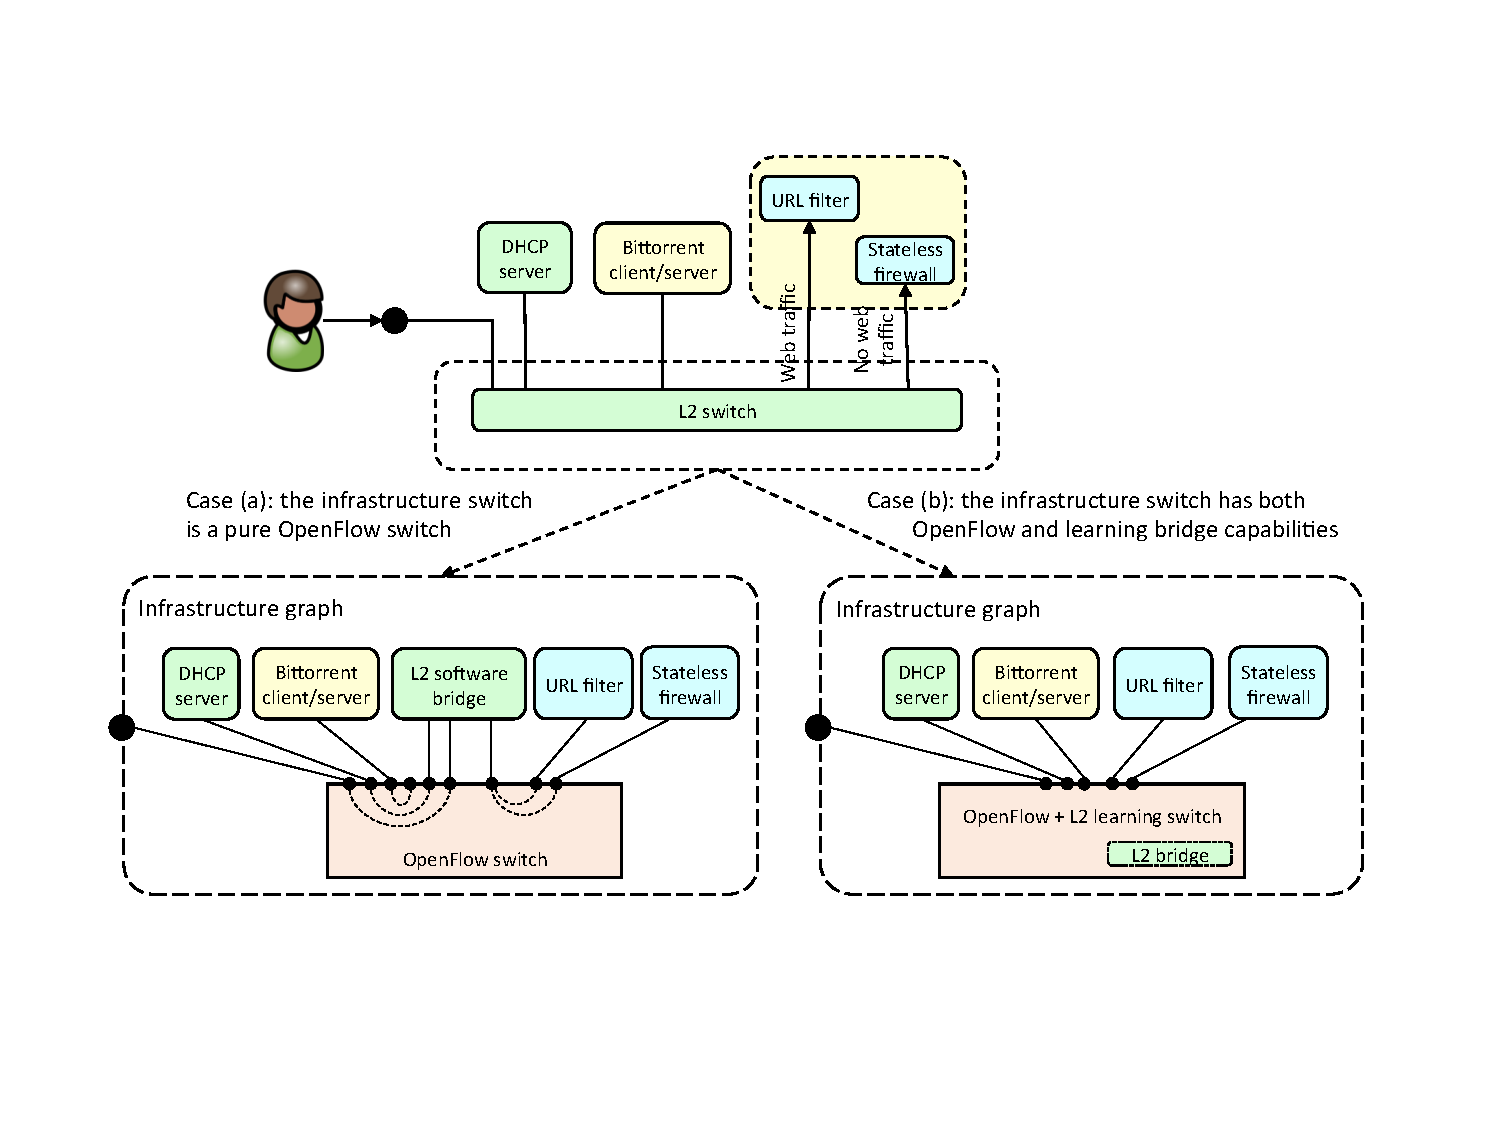
\includegraphics[clip= true, width= \columnwidth, trim= 0cm 1.8cm 0.2cm 2.0cm]{images/NF-FG_reconciliation.pdf}
	\caption{NF-FG - Reconciliation}
	\label{fig:NF-FG_reconciliation}
\end{figure}
\end{comment}

% !TEX root = ../thesis.tex
\chapter{Use case: user defined network services}
\label{sec:use_case}

%\subsection{Scenario}
Chapter~\ref{chap:gen_arch} and Chapter~\ref{chap:data_model} respectively provide a general overview of the architecture and a description of the associated data-models; those concepts could be used in a plenty of different use cases involving multiple actors in defining completely virtualized services. 
In order to provide a concrete use case for these abstract models, in the following of the thesis we consider a particular scenario in which \textit{end users}, such as xDSL customers, can define their own service graphs to be deployed on the wide Internet Service Provider (ISP) infrastructure. 

The ISP controls the entire infrastructure; particularly, it provides a service layer through which the end users can define the SG, the orchestration layer and infrastructure resources.
In addition, the end users devices connect to the network through ISP-controlled equipments (i.e., integrated nodes or OpenStack-based nodes), which represent the entry point of user traffic within the operator network.
%\fabio{sarebbe da spiegare che nel caso fosse un openstack-based node come componeti di openstack avrebbe solo il compute}

Finally, an end user's SG can only operate on the traffic of that particular end user, i.e., on the packets he sends/receives through his terminal device.
On the contrary, the ISP is enabled to define a SG that includes some VNFs that should operate on all the packets flowing through the network; hence, this SG must be shared among all the end users connected to the provider infrastructure.


\section{Challenges}

The use case just introduced presents some interesting challenges to be solved. 

%Looking at the our use case scenario, we could enumerate the steps the systems has to encounter to deploy the requested service.



First, the service layer must be able to recognize when a new end user attaches to the network in order to authenticate the user himself. 
Note that, since the infrastructure layer does not implement any (processing and forwarding) logic by itself, this operation requires the deployment of a specific graph that only receives traffic belonging to unauthenticated users, and which includes some VNFs implementing the user authentication.
Moreover, in order to enable the resource consolidation, this authentication graph should be shared among several end users.

Second, after that the user is authenticated, the service layer must retrieve his SG and then connect it to the ISP graph; particularly, the two graphs must be connected in a way so that the user traffic, in addition of being processed by the service defined by the user himself, is also processed by the VNFs selected by the Internet provider.
This interconnection of several graphs in cascade can be realized by exploiting the graph endpoints elements, which are provided by the SG formalism.

Third, the user SG must be completed with some rules  to inject, in the graph itself, all the traffic coming from/going to the end user terminal, so that the service defined by an end user (only) operates on the packet belonging to the user himself.


The data-model proposed in Chapter~\ref{sec:data_model} could flexibly model such work-flow. All SGs described above (e.g. end-user SG, authentication SG, ISP SG) could separately be defined in an independent way by the different actors involved. The architecture stack assures the deployment of the resulting SG, firstly obtaining the FG by the lowering process and then instruct the infrastructure component through the IG, leveraging the reconciliation process to optimize the whole process.
In particular, a general problematic that looks particularly important in this use-case is represented by SG interconnection. In fact, all cited steps are concerned by a dynamical and sometimes timing-related SG interconnection. Moreover, such interconnection model has to be detached, as is done for VNF definition (Section~\ref{sec:gen_arch}), from infrastructure technology details.
As mentioned before, user devices are connected thanks to rule to his graph, such method allows to attach and cleanly detach the user device dynamically from a certain SG. This may allow the user device to communicate on a certain SG and be unaware detached when a certain event happen (e.g. User device has been authenticated). This abstraction is massively leveraged by the service layer while composing services. 


Finally, the service layer must require (to the lower layers) to deploy the user graph, and to create the proper tunnels on the network infrastructure so that the user traffic is bring, from the network entry point, to the graph entry point, which could have been deployed everywhere on the physical infrastructure.

% !TEX root = ../thesis.tex
\chapter{Prototype implementation}
\label{sec:implementation}

This chapter presents the preliminary implementation of the architecture introduced in Section~\ref{sec:gen_arch}, detailing the components used and the engineering choices that have been made in order to create our prototype. Both global orchestrator and service layer application have been written from scratch in python. Being their webapp are used Gunicorn \cite{gunicorn} ("Green Unicorn") and Falcon \cite{falcon}.
Gunicorn is a Python Web Server Gateway Interface HTTP Server for Unix, whereas Falcon is a Python  minimalist  WSGI framework which allow developers to write Web applications or services without having to handle such low-level details as protocols. First of all a description of our use case is given.
% Scelta dettata dalla semplicita e velocita che si ha  a scrivere programmi in python

\begin{comment}
\section{Use case: user defined network services}
\label{sec:use_case}

%\subsection{Scenario}
Chapter~\ref{chap:gen_arch} and Chapter~\ref{chap:data_model} respectively provide a general overview of the architecture and a description of the associated data-models; those concepts could be used in a plenty of different use cases involving multiple actors in defining completely virtualized services. 
In order to provide a concrete use case for these abstract models, in the following of the thesis we consider a particular scenario in which \textit{end users}, such as xDSL customers, can define their own service graphs to be deployed on the wide Internet Service Provider (ISP) infrastructure. 

The ISP controls the entire infrastructure; particularly, it provides a service layer through which the end users can define the SG, the orchestration layer and infrastructure resources.
In addition, the end users devices connect to the network through ISP-controlled equipments (i.e., integrated nodes or OpenStack-based nodes), which represent the entry point of user traffic within the operator network.
%\fabio{sarebbe da spiegare che nel caso fosse un openstack-based node come componeti di openstack avrebbe solo il compute}

Finally, an end user's SG can only operate on the traffic of that particular end user, i.e., on the packets he sends/receives through his terminal device.
On the contrary, the ISP is enabled to define a SG that includes some VNFs that should operate on all the packets flowing through the network; hence, this SG must be shared among all the end users connected to the provider infrastructure.


\subsection{Challenges}

The use case just introduced presents some interesting challenges to be solved. 

%Looking at the our use case scenario, we could enumerate the steps the systems has to encounter to deploy the requested service.



First, the service layer must be able to recognize when a new end user attaches to the network in order to authenticate the user himself. 
Note that, since the infrastructure layer does not implement any (processing and forwarding) logic by itself, this operation requires the deployment of a specific graph that only receives traffic belonging to unauthenticated users, and which includes some VNFs implementing the user authentication.
Moreover, in order to enable the resource consolidation, this authentication graph should be shared among several end users.

Second, after that the user is authenticated, the service layer must retrieve his SG and then connect it to the ISP graph; particularly, the two graphs must be connected in a way so that the user traffic, in addition of being processed by the service defined by the user himself, is also processed by the VNFs selected by the Internet provider.
This interconnection of several graphs in cascade can be realized by exploiting the graph endpoints elements, which are provided by the SG formalism.

Third, the user SG must be completed with some rules  to inject, in the graph itself, all the traffic coming from/going to the end user terminal, so that the service defined by an end user (only) operates on the packet belonging to the user himself.


The data-model proposed in Chapter~\ref{sec:data_model} could flexibly model such work-flow. All SGs described above (e.g. end-user SG, authentication SG, ISP SG) could separately be defined in an independent way by the different actors involved. The architecture stack assures the deployment of the resulting SG, firstly obtaining the FG by the lowering process and then instruct the infrastructure component through the IG, leveraging the reconciliation process to optimize the whole process.
In particular, a general problematic that looks particularly important in this use-case is represented by SG interconnection. In fact, all cited steps are concerned by a dynamical and sometimes timing-related SG interconnection. Moreover, such interconnection model has to be detached, as is done for VNF definition (Section~\ref{sec:gen_arch}), from infrastructure technology details.
As mentioned before, user devices are connected thanks to rule to his graph, such method allows to attach and cleanly detach the user device dynamically from a certain SG. This may allow the user device to communicate on a certain SG and be unaware detached when a certain event happen (e.g. User device has been authenticated). This abstraction is massively leveraged by the service layer while composing services. 


Finally, the service layer must require (to the lower layers) to deploy the user graph, and to create the proper tunnels on the network infrastructure so that the user traffic is bring, from the network entry point, to the graph entry point, which could have been deployed everywhere on the physical infrastructure.
\end{comment}


\section{The service layer}
\label{sec:service_layer}



\begin{comment}
As introduced in Section \ref{sec:sl_intro}, the service logic and implementation are strictly related to the use case under consideration; in this paper we consider the case in which the \textit{end users} connected to the network define their own services to be applied to the network traffic they generate/receive using their devices.
\end{comment}

In our implementation of the service layer, the \textbf{service layer application (SLApp)} is mostly based on custom code, and it is provided with some APIs to interact with the orchestration layer and with other components required to implement the use case described in Section~\ref{sec:use_case}.

Particularly, it exploits two OpenStack modules: an extended version of \textbf{Keystone} (detailed in Section~\ref{sec:keystone}), and \textbf{Glance} (detailed in Section~\ref{sec:openstack_storage}), used to store the VNF templates.

The choice of Glance to store the templates is not a very good choice,  a better solution could be using \textbf{Swift} (Section~\ref{sec:openstack_storage}), because it is an object storage instead of \textbf{Glance} that is an image repository. We have made this choice only to reduce the number of OpenStack components installed for performance reasons.

According to our use case, at the startup of the infrastructure, the SLApp provides both the ISP graph and the authentication graph to the orchestration layer, which in turn deploys them on one (or more) node(s) available in the infrastructure layer.

It is worth noting that, in addition to the VNFs implementing the authentication graph, the end users authentication process exploits the OpenStack module Keystone (available in our service layer), which has been extended to store the SG, in addition to all the other information needed to authenticate a user.

\begin{comment}
\fabio{The event of a new flow available at one node at the edge of the network, received by the SLApp through a proper API from the lower layers of the architecture, causes the update of the authentication graph, so that it can properly handle the traffic of the new user device.}
Through this API, the SLApp also knows the source MAC address of the new packets, which can be used to uniquely identify all the traffic belonging to the new end user.
Hence, the authentication graph is enriched with a rule matching the specific MAC address; this way, the new packets enter into the graph for the user authentication, wherever the graph itself have been deployed.
Finally, the updated graph is provided to the orchestration layer, which takes care of applying the modifications on the physical infrastructure.
\end{comment}

In the current implementation of SLApp all the user are always connected to the authentication graph through a rule that sends all the traffic to that graph. So the user can immediately reach the authentication web portal and authenticate himself. Whatever the future implementation of SLApp should be able to intercept the event of a new flow available at one node at the edge of the network, and should receive through a proper API from the lower layers of the architecture the update of the authentication graph, so that it can properly handle the traffic of the new user device. Through this API, the SLApp also knows the source MAC address of the new packets, which can be used to uniquely identify all the traffic belonging to the new end user. Hence, the authentication graph is enriched with a rule matching the specific MAC address; this way, the new packets enter into the graph for the user authentication, wherever the graph itself have been deployed.
Finally, the updated graph is provided to the orchestration layer, which takes care of applying the modifications on the physical infrastructure. This modification permits a dynamic connection of users to our network service, and makes it much more flexible.

The user authentication triggers the instantiation of his own SG; at this point, the SLApp retrieves the proper SG description from Keystone, connects it to the ISP-defined SG, and starts the lowering process aimed at translating this high level view of the service into a FG.
In particular, the SLApp executes the ``\textit{control and management network expansion}'' and the ``\textit{LAN expansion}'', as shown in Figure~\ref{fig:network_function_forwarding_graph}(b).
Moreover, it performs the ``\textit{service enrichment}'' step, aimed at connecting the graph with network functions that are needed for the correct delivering of the service defined by the user.
For instance, as already discussed above (Figure~\ref{fig:graphs}(c)), these VNFs may include a DHCP server and a VNF implementing the NAT and router functionalities; although they are not of interest for the end user, these VNFs are automatically added by the SLApp because required for the correct behavior of the network. At this moment the addition of this VNFs is forced by the logic of SLApp, even if this function is already present in user service graph. This would call for a more fine control that is left to future developments.

Before being finally provided to the orchestration layer, the FG is completed with a rule matching the MAC address of the user device, so that only the packets belonging to the user himself are processed into his own graph, as required by the implemented use case. %described in Section~\ref{sec:use_case}.
Moreover, the graph endpoint through which the traffic sent by the end user enters into the graph is associated with the entry point of such traffic in the provider network.
This way, the orchestration layer will be able to configure the network in order to bring the user traffic from its entry point into the network to the node on which the graph is deployed.

As mentioned before, the logic of endpoints connection is managed by the SLApp. Indeed it is in charge of connecting graphs  according to the logic of our use case (described in Section~\ref{sec:use_case}). Hence, when an user graph is instantiated it checks the name of the endpoints, \texttt{"USER\_INGRESS"} for the endpoint that manage the traffic through the user, \texttt{"USER\_EGRESS"} for the endpoint connected to ISP and \texttt{"USER\_CONTROL"} for the endpoint of the control network (inserted by the SLApp). The endpoint named \texttt{"USER\_EGRESS"} will be connected with the endpoint of ISP graph named \texttt{"ISP\_INGRESS"}. This connection is made changing the \texttt{id} of the endpoint with the \texttt{id} of ISP endpoint. Being the endpoints of ISP connected to user a \texttt{one-to-many} endpoint, this requires an update of the ISP graph, which create a new \texttt{one-to-one} endpoint, this update is needed every time a graph is attached to it. In the real implementation, the ISP graph is instantiate with a fixed number of endpoints and no one updates is done, because the current implementation of infrastructure layer does not support updates of endpoints. 

As a final remark, Global orchestrator has to keep track of user sessions, in order to allow a user to connect to his own SG through multiple devices at the same time without any duplication of the graph itself.
In particular, when an already logged-in user attaches to the network with a new device, the SLApp: \textit{(i)} retrieves the FG already created from the orchestration layer; \textit{(ii)} extends it by adding rules so that also the traffic coming from/going to the new device is injected into the graph; \textit{(iii)} sends the new FG to the orchestration layer.




\subsection{Authentication graph}
\label{sec:auth_graph}

The \textit{authentication graph} is required in our use case in order to authenticate an end user when he connects to the provider network with a new device.
In particular, as shown in the left of Figure~\ref{fig:auth_graph}, the SG defined in the service layer consists of a LAN connected to: a VNF that takes care of authenticating the users, a DNS server and a DHCP server.
However, according to its template, the VNF implementing the users authentication actually consists of three VNF images: an Openflow switch, an Openflow controller and a captive portal. 
The resulting FG, completed with a control network, is shown in the right of the picture; as evident from the picture, this graph is connected to the Internet only through the control network, so that end user's traffic cannot go outside of the graph itself.

\begin{comment}
As shown in Figure \ref{}, the FG actually deployed on the infrastructure consists of a DHCP server, a DNS server, an Openflow controller and a web captive portal connected to an Openflow switch\footnote{It is worth noting that the picture also shows the original SG, in which the }
\end{comment}

As detailed above, when an unauthenticated user connects to the network, his traffic is bring to the authentication graph, so that the user can authenticate himself and trigger the instantiation of his own service.
In particular, thanks to the DHCP server and the DNS server, 
%DHCP packets reaches the DHCP server attached to the graph, as well as the DNS queries are handled by the DNS server defined in the graph itself.
%Thanks to these two functions, 
%
the user device retrieves the network parameters and it is able to resolve the names; this way, the user can send HTTP packets and finally start the actual authentication process.
In fact, the HTTP traffic entering into the Openflow switch is sent to the Openflow controller through an Openflow \texttt{packet in} message; this VNF modifies the original MAC and IP destination addresses %(i.e., the MAC address of the default gateway provided by the DHCP server, and the IP address of the web server hosting the required web page got through the DNS server) 
with those of the web captive portal, and then sends back the packet to the Openflow switch, which will provide it to the proper VNF. 
Before responding with a login page, the web captive portal provides a HTTP \texttt{302 temporary redirect} message to the user, in order to notify the client of the redirection and avoiding wrong caching. 

After the user authentication, the web captive portal contacts the SLApp through the control network and triggers the deployment of the proper SG on the infrastructure. In the deployment process the flow that bring the user traffic to its graph is instantiated last, this for maintain the connection with the captive portal until all resources of user graph are deployed. In this way when the user is no longer able to reach the captive portal, he is already connected to a new graph and thanks to a very short lease provided from DHCP of authentication graph, he immediately gets the new address without even noticing the change.

\begin{figure} %[h]
	\centering
	% left bottom right top
	\includegraphics[clip= true, width= 1\columnwidth, trim= 0.0cm 12cm 0.3cm 1.1cm, page= 36]{images/Pictures_definitivo.pdf}
	\caption{Authentication SG and FG.}
	\label{fig:auth_graph}
\end{figure}

%graph deployment in the SLApp which will deploy the SG previously defined by the end user.









\begin{comment}
\subsection{Cascading service graphs}
\label{sec:ep_cascade}

The SG and FG models proposed in this thesis allow the concatenation of many service graphs through the graph endpoints.
To this purpose, each endpoint is associated with an unique identifier and a cardinality, indicating if that endpoint can be used to connect the graph with one or many other graphs, i.e., to implement a \texttt{one-to-one} or a \texttt{one-to-many} interconnection.
Then, before the FG is given to Infrastructure layer, the endpoints are manipulated as follows.
If the connection is between endpoint never connected until now (\texttt{one-to-one} connection) endpoints are let unmodified, while if at least one of endpoints evolved  in the connection are already connected with an other graph (\texttt{one-to-many} connection),  endpoint is connected with a LAN connected with several new endpoints, each one marked as \texttt{one-to-one}, and that will be dedicated to the connection to a single other graph.

To better understand, consider the use case under analysis, which requires that each end user SG is cascaded with a common graph defined by the ISP, so that: \textit{(i)} the packets generated by the end users are processed in the ISP graph before going towards the Internet; \textit{(ii)} the packets coming from the Internet are first handled by the ISP graph, which is then able to provide them to the proper user SG.
%Hence, the following of this section details how these inter-SG connections are implemented in our service layer, by using as an example our use case.

Particularly, referring to Figure~\ref{fig:endpoints}(a), the \textit{egress} endpoint of each user SG must be connected to the \textit{ingress} endpoint of the ISP SG.
As a consequence, the \textit{egress} endpoint of the user graph is marked as \texttt{one-to-one}, while the \textit{ingress} endpoint of the ISP graph is marked as \texttt{one-to-many}. %, since it must be connected to several end user graphs\footnote{Remember, in fact, that the ISP graph is shared among all the end users.}.
Hence, the service layer replaces this last endpoint with several new endpoints connected to a LAN, as depicted in Figure~\ref{fig:endpoints}(b).

\begin{figure} %[h]
	\centering
	% left bottom right top
	\includegraphics[clip= true, width= 0.9\columnwidth, trim= 0.0cm 1.2cm 1.2cm 0.0cm, page= 15]{images/Pictures_definitivo.pdf}
	\caption{Connection of many user SGs to a single ISP SG.}
	\label{fig:endpoints}
\end{figure}


According to Figure~\ref{fig:endpoints}(c), when a user SG is going to be deployed, its endpoint are not expanded, since they are marked as \texttt{one-to-one}.
However, the SLApp creates a logical connection between the \textit{egress} endpoint of the graph itself and one of the new endpoints of the ISP SG.
This way, the orchestration layer (which has no information on the use case implemented by the service layer) knows that the traffic going towards/coming from the Internet must be processed by the ISP SG after/before going towards its final destination, %and that traffic coming from the Internet must enter in the ISP SG before being handled by the service defined by a specific user, 
and hence can instruct the infrastructure layer to create the proper links.

\end{comment}



















\begin{comment}
\section{Cascading service graphs}
\label{sec:ep_cascade}

\fabio{da spostare nel data model quando spiego il service graph}
%\ivano{I'm not sure that this is the right place for this text. Is this a step of the lowering process?}



\fabio{The SG model proposed in this paper allows the concatenation of many service graphs through the graph endpoints.
To this purpose, each endpoint is associated with an unique identifier and a cardinality, indicating if that endpoint can be used to connect the graph with one or many other graphs, i.e., to implement a \texttt{one-to-one} or a \texttt{one-to-many} interconnection.
Then, before the lowering of  the SG into a FG, the endpoints are manipulated as follows.
The \texttt{one-to-one} endpoints are let unmodified, while each \texttt{one-to-many} endpoint is replaced with a LAN connected with several new endpoints, each one marked as \texttt{one-to-one}, and that will be dedicated to the connection to a single other graph.}

To better understand, consider the use case under analysis, which requires that each end user SG is cascaded with a common graph defined by the ISP, so that: \textit{(i)} the packets generated by the end users are processed in the ISP graph before going towards the Internet; \textit{(ii)} the packets coming from the Internet are first handled by the ISP graph, which is then able to provide them to the proper user SG.
%Hence, the following of this section details how these inter-SG connections are implemented in our service layer, by using as an example our use case.

\fabio{Particularly, referring to Figure~\ref{fig:endpoints}(a), the \textit{egress} endpoint of each user SG must be connected to the \textit{ingress} endpoint of the ISP SG.
As a consequence, the \textit{egress} endpoint of the user graph is marked as \texttt{one-to-one}, while the \textit{ingress} endpoint of the ISP graph is marked as \texttt{one-to-many}.} %, since it must be connected to several end user graphs\footnote{Remember, in fact, that the ISP graph is shared among all the end users.}.
Hence, the SLApp replaces this last endpoint with several new endpoints connected to a LAN, as depicted in Figure~\ref{fig:endpoints}(b).

\fabio{According to Figure~\ref{fig:endpoints}(c), when a user SG is going to be deployed, its endpoint are not expanded, since they are marked as \texttt{one-to-one}.
However, the SLApp creates a logical connection between the \textit{egress} endpoint of the graph itself and one of the new endpoints of the ISP SG.
This way, the orchestration layer (which has no information on the use case implemented by the service layer) knows that the traffic going towards/coming from the Internet must be processed by the ISP SG after/before going towards its final destination, %and that traffic coming from the Internet must enter in the ISP SG before being handled by the service defined by a specific user, 
and hence can instruct the infrastructure layer to create the proper links.}

\end{comment}

\section{Global orchestrator}
%\section{The global orchestrator}
\label{sec:global_orch}


As depicted in Figure~\ref{fig:orchestrator}, the \textbf{global orchestrator} corresponds to the first two levels of the orchestration layer, and consists of %two parts: one technology dependent, the other technology independent.
a technology dependent part and a technology independent part.
This module receives the FG created by the service layer through the northbound API, manipulates it and sends the resulting FG(s) to the proper infrastructure controller(s).
It is worth noting that our architecture consists of a single global orchestrator that sits on top of many physical nodes, even implemented with different technologies (e.g., the integrated node and the OpenStack-based node).

When the technology independent part of the global orchestrator receives the FG, it executes the following operations.

First, for each VNF specified in the graph, it retrieves a description of the function itself (i.e., its template) from Glance
as detailed in Section~\ref{sec:template}, the template contains information such as the amount of CPU, RAM and disk required by the VNF
but it could also specify that the VNF is actually a sub-graph composed by other VNFs.
In this case, the technology independent part of the global orchestrator executes the ``\textit{VNFs expansion}'' step depicted in Figure~\ref{fig:graphs}(d), and retrieves the description of the new VNFs (which, in turn, could be recursively expanded in further VNFs).
Then, the ``\textit{consolidation}'' step of the lowering process is performed, 
%all the L2 switch VNFs connected together are consolidated into a single one, 
so that the FG is simplified as shown in Figure~\ref{fig:graphs}(e). 

At this point, the global orchestrator schedules the FG on the proper node(s) of the physical infrastructure.
Although the general model presented in Section~\ref{sec:general_orch} supports a scheduling based on parameters such as CPU and memory requirements of the VNFs, KQIs (e.g., maximum latency, expected throughput) and high level policies, such a scheduler is let as a future work.
In fact, in our first implementation of the global orchestrator, it simply instantiates the entire FG on the same node used as a network entry point for the traffic to be injected into the graph itself.

The resulting FG is then provided to the proper control adapter, according to the technology implementing the node of the infrastructure layer on which the graph is going to be scheduled.
%the physical infrastructure on which the graph itself is going to be scheduled.
So far, two control adapters have been defined, in order to support the deployment of FGs into OpenStack domains and into integrated nodes; these adapters take care of translating the FG provided by the technology independent part into a formalism accepted by the proper \textit{infrastructure controller}, which is in charge of sending the commands to the infrastructure layer.
Moreover, they convert the endpoints of the graph into physical ports of the node on which it is going to be deployed and, if required, instruct the infrastructure controller to create a GRE tunnel on the infrastructure layer.
This tunnel could be used to connect together two pieces of the same service but deployed on different nodes of the infrastructure layer; %, as well as it can be created because required by the service layer.
according to our use case, a GRE tunnel is required when the FG associated with an end user is deployed on a different node than the one used by his traffic to enter in the provider network, but also to bring the traffic generated by new end users to the authentication graph.
However, since the current implementation of the scheduler never splits a graph in multiple parts, and deploys the graph on the node through which the traffic enters into the network, this feature is never exploited by the global orchestrator.

As a final remark, the global orchestrator also supports the updating of existing graphs. 
In fact, when it receives a FG from the service layer, it checks if this graph (i.e., a FG with the same identifier) has already been deployed; in this case, both the FGs (the one deployed and the new one) are provided to the proper controller adapter, which sends to the infrastructure layer:
% Non e vero l'interfaccia dei component adapter e uguale, quindi si invia a tutti e due entrabi i FG, sara poi ne CA dell'integrated node che si fara il diff.
\textit{(i)} the difference between the two graphs in case of integrated node, or \textit{(ii)} both the FGs in case of OpenStack-based node (As described in Section~\ref{sec:os-proto}, in this case the difference is already calculated by the Heat module of OpenStack). Furthermore a graph update is done when it receive a graph with an endpoint ID equal to that of an other already instantiate. In particular this endpoint is instantiated in a different node. So, when the service layer attaches two graphs and this two graphs are instantiated in different nodes. In this case the orchestrator should update the old endpoint with the information needed to connect it to the other endpoint (i.e. information needed to create a tunnel GRE), and enrich the new endpoint with the same information.






\section{The integrated node}
%\section{The integrated node}
\label{sec:single_server_proto}



This section describes the \textbf{integrated node}~\cite{demobudapest}, i.e., a node of the infrastructure layer consisting of a single physical machine mainly running dedicated software; the overall architecture of this implementation is provided in Figure~\ref{fig:proto_unify}.
Each integrated node is independent from the other nodes of the infrastructure layer and hence, as shown in the figure, its infrastructure controller can be \textit{integrated} on the same server running the VNFs of the graphs. 


Going into details, the FG is received through a REST API by the \textbf{node resource manager}, which is the component that takes care of instantiating the graph on the node itself; this requires the execution of the reconciliation process, to start the proper VNF images (downloaded from a \textbf{VNFs repository}) and to configure the paths among them.
Particularly, the last two operations are executed through two specific modules of the node resource manager, namely the \textbf{compute controller} and the \textbf{network controller}.






\begin{figure}%[h]
	\centering
	% left bottom right top
	\includegraphics[clip= true, width= 0.8\columnwidth, trim= 0.6cm 2.3cm 1.3cm 1.0cm, page = 16]{images/Pictures.pdf}
	\caption{Logical architecture of the integrated node.}
	\label{fig:proto_unify}
\end{figure}


According to Figure~\ref{fig:proto_unify}, the traffic steering among the VNFs is based on \textbf{xDPd}~\cite{xdpdwebsite}, a framework that supports the dynamic creation of several (pure) Openflow switches called \textbf{Logical Switch Instances (LSIs)}; each LSI can be connected to physical interfaces of the node, to VNFs, and to other LSIs.
In the prototype, a different LSI (called \texttt{tenant-LSI}) is dedicated to steer the traffic among the VNFs of a specific graph, while the \texttt{LSI-0} is in charge of classifying the traffic coming from the network (or from other graphs) and of delivering it to the proper \texttt{tenant-LSI}. %graph implementation.
The \texttt{LSI-0} is the only one allowed to access the physical interfaces, and the traffic flowing from one \texttt{tenant-LSI} to another has to transit through the \texttt{LSI-0} as well.

Being the LSIs Openflow switches, the rules describing how to steer the traffic in the graph are translated into Openflow \texttt{flowmod} messages.
Moreover, since the LSIs are \textit{pure} Openflow switches, the reconciliation process described in Section~\ref{sec:ig} does not remove the VNFs implementing the L2 switch, which are then implemented using the proper software images and are not mapped on the vSwitch used to interconnect the components of the graph.

When a FG description (either a new one or an update of an existing FG) is received by the node resource manager, this module:
%\textit{(i)} replaces the generic endpoints with physical ports of the server; 
\textit{(i)} retrieves a software image for each VNF required and installs it; \textit{(ii)} instantiates a \texttt{tenant-LSI} on xDPd and connects it to the \texttt{LSI-0} and to the proper VNFs; \textit{(iii)} crates an OpenFlow controller that is exploited to insert forwarding rules into the flow table(s) of the new LSI, in order to steer the traffic among the VNFs as required by the graph.
In particular, the rules defining the paths among VNFs (and physical ports) originates two sequences of Openflow \texttt{flowmod} messages: one to be sent to the \texttt{LSI-0}, so that it knows %which traffic must be provided to the \texttt{tenant-LSI} and how to treat packets coming from this LSI; 
how to steer traffic among the graphs deployed on the node and the physical ports; the other used to drive the \texttt{tenant-LSI}, so that it can properly steer the packets among the VNFs of a specific graph.

It is worth noting that, when a new flow enters into the \texttt{LSI-0}, it provides the new packets to its own Openflow controller through an Openflow \texttt{packet in} message; at this point the Openflow controller, through the network controller, notifies the upper layers of the architecture of this event, which will react properly according to the use case implemented in the service layer.

The integrated node supports three flavors of VNFs: DPDK processes~\cite{dpdk}, VNFs deployed in Docker containers~\cite{docker}, and VNFs running in VMs.
While the former type provides better performance (in fact, an LSI exchanges packets with DPDK VNFs with a zero-copy mechanism), Docker containers and VMs guarantee properties such as isolation among VNFs, as well as they allow to limit the CPU and memory usage of VNFs themselves. 

As a final remark, the integrated node has been designed having in mind a network aware scheduling of the VNFs on the cores available on the physical machine, although this feature has not been implemented yet in our current prototype.
In fact the node resource manager, which takes care of both deploying the VNFs and configuring the vSwitch to properly steer the traffic among them, receives the entire FG at the same time from the upper layer, which describes both the VNFs to be executed and the paths among them.
As a consequence, this module could schedule the VNFs in a way to optimize the packets flow among the functions themselves and between the VNFs and the NICs, by taking into account the way in which they are interconnected within the FG.



















\section{The OpenStack-based node}
%\section{The OpenStack-based node}
\label{sec:os-proto}


This section presents the \textbf{OpenStack-based node}, a node of the infrastructure layer consisting of a cluster of servers within the same OpenStack domain.
As shown in Figure~\ref{fig:proto_openstack}, all the physical machines of the cluster are managed by a single infrastructure controller, which is composed of a number of OpenStack modules and a SDN controller. 

\begin{figure}%[h]
	\centering
	% left bottom right top
	\includegraphics[clip= true, width= 1\columnwidth, trim= 0in 0.8in 0.0in 0in, page = 24]{images/Pictures_definitivo.pdf}
	\caption{OpenStack-based node.}
	\label{fig:proto_openstack}
\end{figure}

Openstack usage in our architecture represents an interesting choice for legacy compatibility, as well as it allows us to reuse all the features it already implements.
However, since OpenStack was designed to support the deployment of cloud services,  several modifications have been done in order to enable the deployment of FGs as well, in order to use it in our architecture. Any changes made to OpenStack are designed to keep the legacy behavior.
These modifications, as well as the operations executed to instantiate the FG are described in the following of this section.

As depicted in Figure~\ref{fig:proto_openstack}, to implement the {OpenStack-based node and its infrastructure controller we use the following components: \textit{(i)} \textbf{Nova}, which is the compute service; \textit{(ii)} \textbf{Neutron}, namely the network service; \textit{(iii)} the orchestration layer, called \textbf{Heat}; \textit{(iv)} the repository for virtual machine (VM) images, called \textbf{Glance}.
Openstack is able to start \textbf{VMs} by interacting with a wide range of different hypervisors (e.g. KVM, Xen, VMware); moreover, in order to properly steer the traffic between the several servers under its control, it can be integrated with a SDN controller: in our prototype we use \textbf{OpenDaylight (ODL)} (Section~\ref{sec:opendaylight}). 
As evident from the picture, Heat, Nova scheduler, Nova API, Neutron and ODL compose the infrastructure controller, while each physical machine executing the VNFs is a Nova compute node, which runs a Nova compute agent, \textbf{Open vSwitch (OVS)}~\cite{ovswebsite} and the \textbf{KVM hypervisor}.

	
When the global orchestrator decides to deploy a FG in an OpenStack-based node, the proper control adapter translates the FG description into a format supported by Heat, performing a reconciliation step that removes, from the graph itself, all the VNFs implementing the L2 switch, since this functionality will be mapped on the OVS instances running on the physical servers. In fact, OVS is not pure Openflow switch: it is both able to forward traffic based on traffic steering rules as well as to implement the MAC learning algorithm.
The current control adapter despite OpenStack uses OVS, has not yet been implement the reconciliation process because OpenStack manages  isolation between networks with VLANs. This means that if the user traffic enters through the switch (to reconcile) the port where the user traffic comes from must be an access port that tags traffic with the right tag belong to the \texttt{neutron} network. 
To be used in our prototype, Heat has been extended in order to support the \texttt{flow-rule} primitive, which describes how to steer the traffic between the ports of the VNFs composing a graph.
This primitive provides an interface similar to the OpenFlow~1.0 \texttt{flowmod}; however, it allows the traffic steering between virtual ports without knowing in advance the physical server on which the respective VNFs will be scheduled.
	
As soon as Heat receives the FG, it sends a sequence of commands to Nova for each VNF of the graph in order to deploy and start the VNF itself; at this point, the Nova scheduler \textit{(i)} selects the physical server on which the VNF must be deployed using the standard OpenStack ``filter \& weight'' algorithm, \textit{(ii)} sends the proper command to the Nova compute instance on the selected node, which in turn \textit{(iii)} retrieves the VNF image from Glance and finally \textit{(iv)} starts the VM.Note that no modification is done in Nova compute, in order to support the deployment of the FGs.
The scheduling algorithm over cited is very simple and consists of two steps: in the first one, all the Nova compute nodes are considered, and those that are not able to run a VM are filtered (e.g., because the VM requires an hypervisor that is not available on the node). 
In the second phase, a weight is associated with each one of the remaining servers, and the one with higher weight is selected to run the VM.
The weights are calculated by considering the resources available on the machine.
It is worth noting that Nova scheduler has two limitations: \textit{(i)} it schedules a VNF as soon as it receives the command from Heat; \textit{(ii)} it does not have any information on the paths among the VNFs in the graph.
As a consequence, the FG could be split on the available compute nodes without taking into account the paths among the VNFs, resulting in suboptimal performance.

	
After that the VMs implementing the required VNFs have been started, Heat sends a \texttt{flow-rule} at a time to Neutron, which takes care of creating the proper connections among these VNFs.
Hence, also Neutron has been extended to support the \texttt{flow-rule} primitive, in addition to the standard abstractions used to implement traditional L2 networks (e.g., broadcast domains, IP subnets, ports).
It is worth noting that our \texttt{flow-rule} is functional equivalent to the Neutron official traffic steering extension~\cite{neutronsteeringofficial}.
However, it has not been used in our prototype because: \textit{(i)} its implementation is not available (at the beginning of November 2014) while our demo of traffic steering in OpenStack was released in July; \textit{(ii)} it does not support ports that are outside the OpenStack domain.
When Neutron receives a \texttt{flow-rule}, starting from the network topology (retrieved through ODL) it creates a set of openflow-like rules and sends those to ODL.
At this point, the \texttt{flowmods} are created to OpenDayLight, which sends them to the proper switches; note that these switches could be either inside a Nova compute node, or physical switches used to interconnect several servers, in case the VNFs have been instantiated by the Nova scheduler on many compute nodes.

\begin{comment}
\fabio{dire del problema di openstack che tutti i pacchetti escono dal nodo network}
\end{comment}	

To conclude, the OpenStack-based node notifies the upper layers of the architecture, when a new flow (belonging to  a new device) enters into the node itself.
As already stated above, this information may be exploited by the service layer logic in order to implement a specific use case.
	
\section{Discussion: Openstack-based node vs. integrated node}


\renewcommand{\arraystretch}{1.5}
\begin{table}[tb]
%\begin{table*}[!t]
	\centering
	\tiny

	\caption{Integrated vs OpenStack-based node.}
	\label{tab:features}
	\begin{tabular}{c||c|c|}
		%\toprule
		%\multirow{2}{*}{\textbf{Attack settings}} & 
		%&	\multicolumn{2}{c}{\textbf{Ping (avg) [ms]}} & \multicolumn{2}{c}{\textbf{File transfer [s - MBps]}}\\ & \textit{One user} & \textit{Two users} & \textit{One user} & \textit{Two users}\\
		& Integrated node & OpenStack-based node \\
		\hline	
		%	\textbf{Compatible with existing cloud environments} & no  &  yes \\	
		\textbf{Compatible with existing} & no  &  yes \\	
		\textbf{cloud environments} &  &  \\	
		%\textbf{No service} &  28.78 &  & 81 - 7.08& - \\
		\hline
		%	\midrule
		%	\midrule
		%\textbf{OS one compute node} & 29.40 & 30.24 (usr1) / 35.26 (usr2)  & 570 - 1 & 614 - 0.95 (usr1) / 767 - 0.76 (usr2) \\
		%	\midrule
		\textbf{Complete control of the FG} & yes & no (due to the network node) \\
		\hline
		%\textbf{OS two compute nodes}  & 24.8 & 31.24 (usr1) / 25.76 (usr2)  & 1566 - 0.37 & 1833 - 0.31 (usr1) /  13621 - 0.04 (usr2) \\
		\textbf{Support to smart scheduling of the FG} & possible & requires many changes to the internals of OpenStack \\
		\hline
		%\textbf{Integrated node} & 30.08  & 33.67 (usr1) / 33.13 (usr2) & 314 - 1.82 & 647 - 0.91 (usr1) / 807 - 0.72 (usr2) \\
		\textbf{Type of VNFs} & Docker containers, DPDK processes,  & Virtual machines, \\
		& Virtual machines &  Docker containers (not completely supported)\\
		\hline
		%	\bottomrule
	\end{tabular}
%\end{table*}
\end{table}
Table~\ref{tab:features} summarizes the main features of the Integrated node and of the OpenStack-based node, as well as it shows the main differences among them.  
As evident from the table, unlike the integrated node, the OpenStack-based node supports the deployment of a FG in a cloud environment, in which a single OpenStack instance manages a cluster of physical servers (like in boxes on the right of Figure~\ref{fig:target_scenario}) called Nova compute nodes. Further OpenStack manages also the case of an edge box, like boxes on the left of Figure~\ref{fig:target_scenario}. This because it permits the instantiation of the only \texttt{compute node} on this boxes and instead the \texttt{controller node} and a \texttt{network node} in the remote server.

\begin{figure}%[h]
	\centering
	% left bottom right top
	\includegraphics[clip= true, width= 1\columnwidth, trim= 0in 0in 0.0in 0in, page = 40]{images/Pictures_definitivo.pdf}
	\caption{Target scenario.}
	\label{fig:target_scenario}
\end{figure}


However, it has several limitations compared to the integrated node, as described in the following.

First, the upper layers do not have the complete control on the service actually deployed in an OpenStack-based node since, as described in Section~\ref{sec:os-proto}, each OpenStack domain is connected to the Internet through the so called \textit{network node}.
As a consequence, packets towards/from the Internet are handled by the functions running in this component (e.g., the NAT, the router), before/after being actually processed by the VNFs implementing the required service.

Moreover, according to Section~\ref{sec:single_server_proto}, the integrated node could potentially schedule the VNFs on the available cores in a way that considers the connections between these VNFs in the graph, in order to improve the performance of the system. 
This optimization is possible because the node resource manager receives the entire FG description at the same time, and hence it has all the information related to the VNFs required and the paths among them, before actually deploying the VNFs themselves.
Instead, in an OpenStack-based node, the entire graph description is only received by Heat, and not by the components actually starting the VNFs and creating the paths on the vSwitch(es).
In particular, the Nova compute agent receives the commands to start the VNFs one at a time, and it does not receive informations among the paths among them at all; in fact, this information is received by the OVS running on the physical servers through an Openflow connection established with OpenDaylLight.

Similarly, the Nova scheduler (which sits on top of all the physical machines belonging to an OpenStack domain) receives the information related to the VNFs to be started one at a time, while it does not receives the connection among them at all; as a consequence, it cannot select the compute node on which a VNF must be instantiated based on the connection among the VNFs in the FG.
%way in which the VNFs are connected in the graph to be deployed.

It is worth pointing out that, currently, this network aware scheduling is neither implemented in the integrated node, nor in the OpenStack-based node; however, while it can be easily introduced in the former prototype, it would require many modifications to the internal operations of OpenStack, in order to be implemented in the Nova scheduler and in the Nova compute node.

Another difference between the integrated node and the OpenStack-based node is in the type of VNFs supported.
Particularly, while former node supports VNFs implemented as Docker containers, VMs and DPDK processes, the latter only runs VNFs within virtual machines.
In fact, although Docker is officially supported by OpenStack, we encountered some limitations in using it in our architecture
% !TEX root = ../thesis.tex
\chapter{Prototype validation}
\label{sec:validation}

To validate the architecture described in the thesis, we carried out several tests aimed at both testing the functionalities implemented, and to measure the performance of the infrastructure layer in terms of throughput, latency introduced and resource required.
%The tests were repeated both with an infrastructure layer consisting of a single integrated node, as well as in case of an OpenStack cluster composed by two compute nodes.
%in case it consists of two servers under the same OpenStack domain.
%Note that, in the latter case the graphs are split so that the VNFs are distributed between the two physical servers.
\begin{comment}
Moreover, during the tests the end users are connected to the infrastructure through a common wireless interface, while their SGs are cascaded to a common graph defined by the ISP and that provides connectivity to the Internet, as depicted in Figure~\ref{fig:deployed_graphs}. 
\end{comment}

\section{Service overview}

The FGs deployed in the tests are shown in Figure~\ref{fig:deployed_graphs}; according to our use case implementation, these graphs include the authentication graph used to authenticate new end users connected to the network, and the ISP graph, which provides connectivity to the Internet and is crossed by the traffic generated from/going towards all the end users.
The control network of this ISP graph  also includes a firewall, so that only the authorized entities (e.g., the ISP itself) can control and configure the deployed VNFs.

\begin{figure}%[h]
	\centering
	% left bottom right top
	\includegraphics[clip= true, width= 0.8\columnwidth, trim= 0in 0.2in 0.0in 0.6in, page= 29]{images/Pictures_definitivo.pdf}
	\caption{Use case scenario.}
	\label{fig:deployed_graphs}
\end{figure}

As evident from the picture, each end user graph provides an example of traffic steering, since it requires that the packets towards the Internet is split so that the web traffic is provided to a traffic monitor and then to a firewall that blocks the HTTP GET towards specific URLs, while the other packets simply traverse a second traffic monitor VNF.
It is worth noting that, thanks to the control interface of the traffic monitors we are able to observe the packets flowing through the specific VNF, and hence to validate the correct behavior of the traffic steering mechanism.

During the tests carried out on the OpenStack-based node, the VNFs are implemented as VMs running on the KVM hypervisor and in a second OpenStack-based node VNFs are implemented in Docker containers.
Instead, in the tests with the integrated node, the firewall is implemented as a DPDK process, while all the others VNFs are implemented in Docker containers.
In particular, both the VMs and the Docker containers run an Ubuntu operating system, and the VNFs are implemented through \textit{standard} Linux tools (e.g., iptables).


As a final remark, according to our use case and the current implementation of the architecture, the end users are directly connected to the node on which their graphs are deployed. %; \textit{(ii)} the user graphs are cascaded to a common graph defined by the ISP and that provides connectivity to the Internet, as depicted in Figure~\ref{fig:deployed_graphs}. 

\section{Performance evaluation}
This section shows the tests executed in order to measure the performance obtained with the preliminary implementation of our architecture.

During the tests, a machine is dedicated to the execution service layer (i.e., service layer application, Keystone) and the global orchestrator; it is equipped with 16 GB RAM, 500GB HD, Intel i7-2620M @ 2.7 GHz (one core plus hyperthreading) and OSX 10.9.5, Darwin Kernel Version 13.4.0, 64 bit, which is the same for both the infrastructure nodes.

The infrastructure layer is implemented on a set of servers with 32 GB RAM, 500GB HD, Intel i7-3770 @ 3.40 GHz CPU (four cores plus hyperthreading) and Ubuntu 12.04 server OS, kernel 3.11.0-26-generic, 64 bits.
In case of OpenStack-based node, a first machine hosts the infrastructure controller (Heat, Nova scheduler, Nova API, Neutron and ODL), the network node, while another one is dedicated to the implementation of the Nova compute node, connected through a Gigabit Ethernet link. In addition to the nova compute that runs VMs another one node, that runs Docker container, is connected in the same OpenStack domain.
%In case of OpenStack-based node, a first machine hosts the infrastructure controller (Heat, Nova scheduler, Nova API, Neutron and ODL), the network node, as well as it acts as a Nova compute node, while another one is dedicated to the implementation of the second Nova compute node, connected through a Gigabit Ethernet link.
In case of the integrated node, one of those machines executes all the software.

The memory required by the different components of the system is reported in Table~\ref{tab:memory}, in which the consumption related to the Nova compute node and to the integrated node has been measured without any VNF deployed.


\renewcommand{\arraystretch}{1.5}
\begin{table*}[htbp]
	\centering
	\tiny
	\caption{Memory consumption.}
	\label{tab:memory}
	\begin{tabular}{c|c}
		%\toprule
		\textbf{Component} & \textbf{Memory [MB]} \\
		\hline	
		\hline
		Service layer + global orchestrator & \\
		(SLApp + Keystone + Horizon + & 558.2\\
		additional (minor) libraries/components)  & \\
		\hline
		Infrastructure controller & \\
		(Heat + Nova scheduler + Nova API + Neutron + ODL + & 3396.7\\
		additional (minor) libraries/components) &  \\
		\hline
		Nova compute node & \\
		(Nova compute + OVS +  & 294.8\\
		additional (minor) libraries/components) &  \\
		\hline
		Integrated node & 120.5\\
		(node resource manager + xDPd + additional (minor) libraries) & \\
		\hline 
		%	\bottomrule
	\end{tabular}
\end{table*}

As evident, the infrastructure controller for the OpenStack-based node is the heaviest component, while the requirements of the integrated node, which is almost based on ad hoc modules, is quite reduced.




\subsection{Deployment time}
%The conditions in that we repeated the tests is the follow: \textit{(i)} user device and server directly connected using a gigabit Ethernet link; \textit{(ii)} user devices connected, through a gigabit Ethernet network, to the node on which the graphs are deployed, which is in turn connected to the server through gigabit Ethernet link.
%Moreover, as node running the VNFs, we used:  an OpenStack-based node with a single server that runs VMs,  an OpenStack-based node consisting of two servers connected with a gigabit Ethernet link VMs, an OpenStack-based node with a single server that runs docker, and the integrated node.

The first kind of tests performed is concerned about the measuring of service deployment time. The table~\ref{tab:fg_istatiatiotion_evaluation}
shows the times of instantiation of the user service graph detailed before, and the transitory time between the instantiation of the graph and the time in which the user is able to ping the server. It also shows the total time of the SG deployment, as we can see, those times are anything but low. What appears to be obvious looking at the Table~\ref{tab:fg_istatiatiotion_evaluation} is that, the imputable for those results is the infrastructure layer, which is in charge of both VMs/dockers instantiation and the creation of paths between them.
It is worth pointing out that this time does not include the download of the VNF images from the repository, which are already cached on the physical nodes.
%
\renewcommand{\arraystretch}{1.5}
\begin{table*}[htbp]
	\centering
	\tiny
	\caption{Deployment time.}
	\label{tab:fg_istatiatiotion_evaluation}
	\begin{tabular}{c|c|c|c|c|c}
		%\toprule
		\textbf{Component} & Service layer & Global orchestrator & Infrastructure layer & Ping & \textbf{Tot} \\
		\hline	
		\hline

		Openstack single node & 0.83 & 0.61 & 127 & 49 & 177.44\\
		(virtual machine)  & & & & & \\
		\hline

		%Openstack two nodes & X & X & 132 & 183 & X\\
		%(virtual machine) & & & & & \\
		%\hline

		Openstack sigle node  & 0.83 & 0.61 & 82 & 13 & 96.44\\
		(docker) & & & & &\\
		\hline
		% SLApp + orch = 1.32
		Integrated node & 0.83 & 0.49 & 72.67 & 11 & 84.99\\
		
		\hline 
		%	\bottomrule
	\end{tabular}
\end{table*}

This test has been repeated using different graphs with a variable number of VNFs and the results are shown in Figure~\ref{fig:startup_times}. All the VNFs use the same image, and all nodes used for the test have it stored locally. One OpenStack node uses VMs that run an Ubuntu Server 12.04 and the size of the image is 1.6 GB. The other one OpenStack node and the integrated node use the Docker containers that run an Ubuntu Server 12.04 and the size of the image is 0.324 GB. Furthermore, in both VMs and Docker containers are used linux bridges to forward of traffic between the vNICs. In these tests the ping time is not considered. Hence, this means that after the time shown in Figure~\ref{fig:startup_times} the user is not immediately able to access to his service. Indeed, as we can see looking the ping value in Table~\ref{tab:fg_istatiatiotion_evaluation}, especially in OpenStack with VMs, the time for starting the services is very high.
%
\begin{figure}[H]
	\centering
	% left bottom right top
	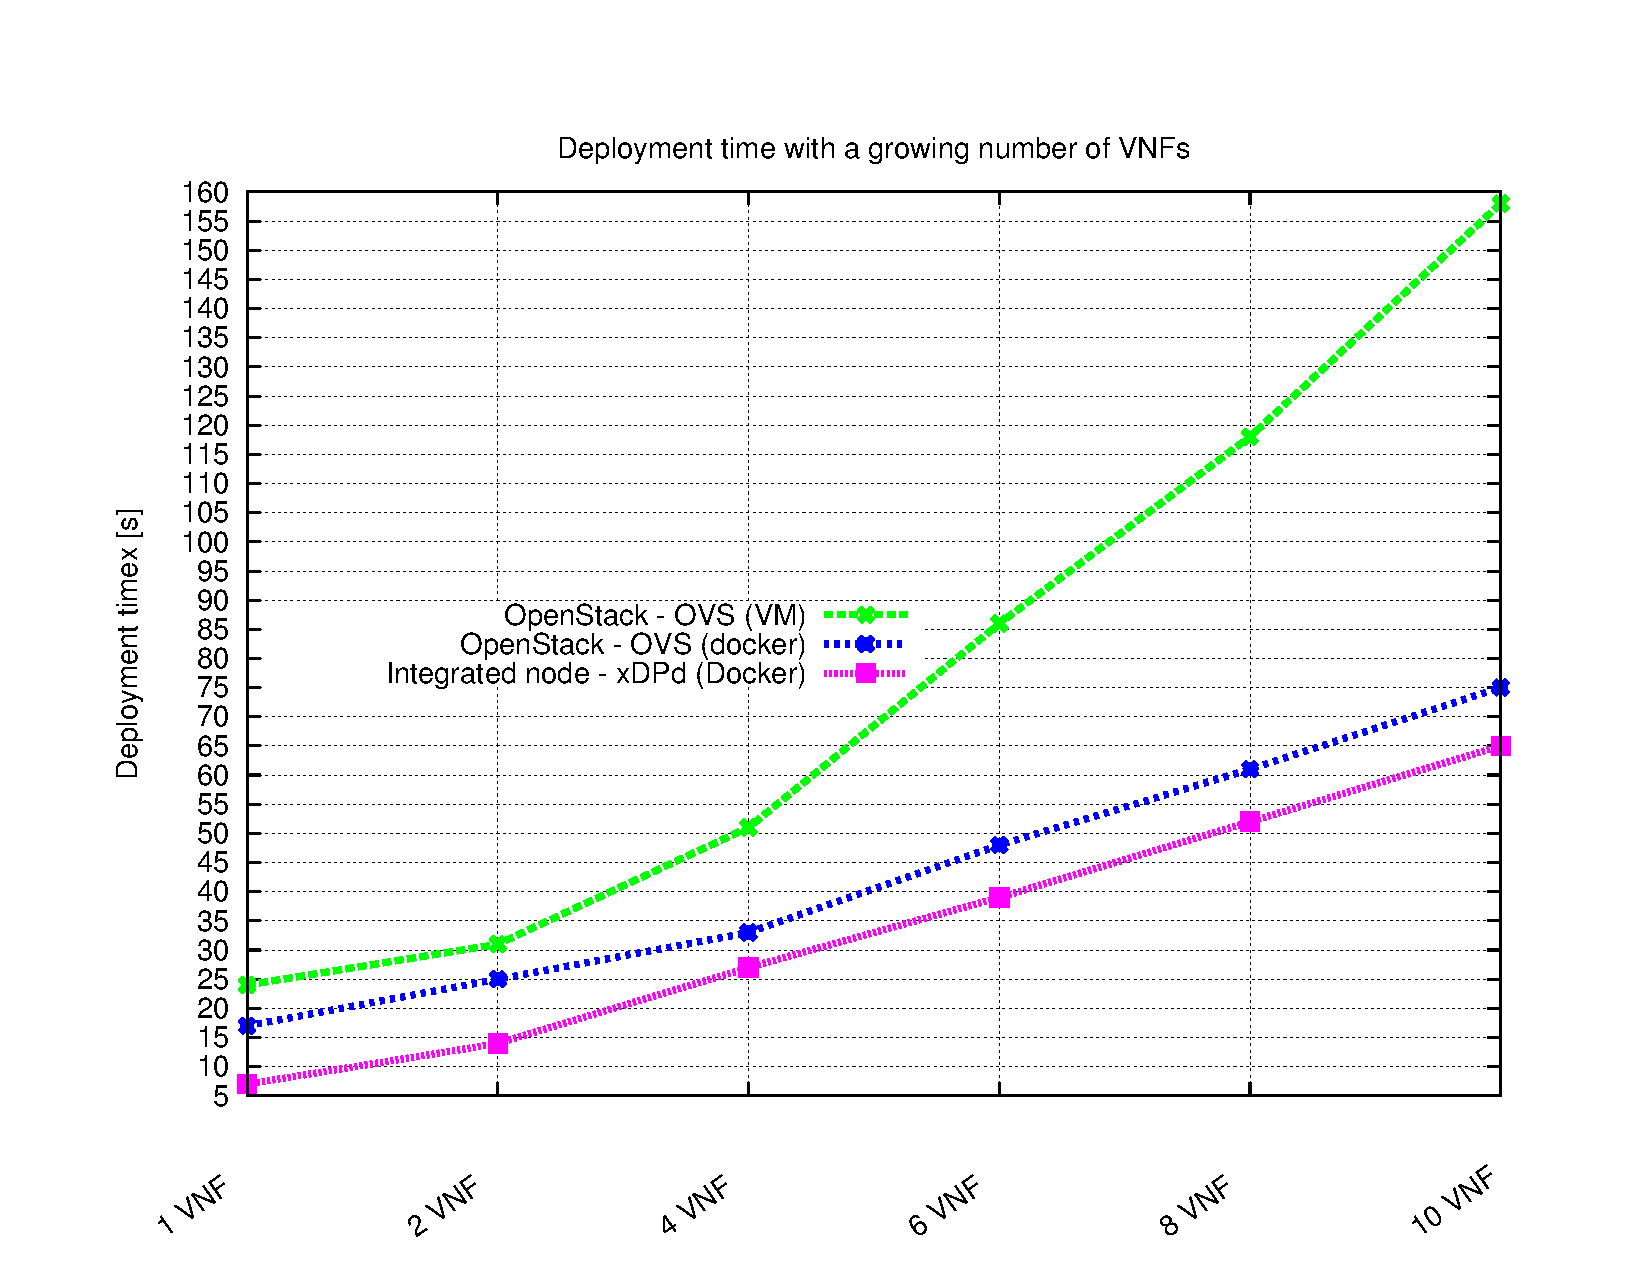
\includegraphics[clip= true, width=0.5\columnwidth]{images/graphs/startup_times.pdf}
	\caption{Startup times.}
	\label{fig:startup_times}
\end{figure}
%
Anyway these performance show a behavior almost linear according to a growing number of VNFs.






\subsection{Throughput and latency}

The second phase of performance evaluation has been dedicated to analyze the throughput that we can achieve on the different infrastructure layers. As shown on the left of the Table~\ref{tab:evaluation}, the different infrastructure layers used are \textit{(i)} OpenStack-based node that runs virtual machines, \textit{(ii)}  OpenStack-based node that runs Docker container, and \textit{(iii)} the integrated node. Also the tests of Figure~\ref{tab:evaluation} are performed connecting directly the user and the server machine. %As shown in Table~\ref{tab:evaluation}, we repeated the tests in the following conditions: \textit{(i)} user device and server directly connected using a gigabit Ethernet link; \textit{(ii)} user devices connected, through a gigabit Ethernet network, to the node on which the graphs are deployed, which is in turn connected to the server through gigabit Ethernet link.
%Moreover, as node running the VNFs, we used: an OpenStack-based node that using VMs, an OpenStack-based node that using VMs, the integrated node.
The first test carried out aims at measuring the latency introduced by the deployed services (Figure~\ref{fig:deployed_graphs}); in particular, the user device(s) sends 100 \texttt{ping} towards the server, and the results were averaged and reported in the left part of the table.
%\footnote{It is worth noting that, according to the deployed SGs, packets exchanged in this test are not handled by the firewall VNF, which only operates on HTTP traffic.}.
The second and third tests are made on TCP traffic so they are most interested about perception of quality of service by end user. In particular the second test aimed at measuring throughput obtained during the download of a file of 4 GB from the server, and it is performed using  \texttt{wget}, a Linux tool that uses the HTTP protocol. Whilst the third test is done using \texttt{iperf}, a network testing tool that can create TCP and UDP data streams and measure the throughput of a network that is carrying them. Finally, the last test is performed for evaluate the performance on UDP traffic, even in this case has been used \texttt{iperf}.
As a consequence, according to the user graph, while the ping are not handled by the firewall, this VNF is instead involved during the file transfer.
%
%
\renewcommand{\arraystretch}{1.5}
\begin{table*}[!htbp]
	\centering
	\tiny
	\caption{Performance of the infrastructure layer.}
	\label{tab:evaluation}
	\begin{tabular}{l||c|c|c|c||}
		%\toprule
		%\multirow{2}{*}{\textbf{Attack settings}} & 
		& \textbf{Ping (avg) } & \textbf{File transfer (wget) }& \textbf{TCP test (iperf)}  & \textbf{UDP test (iperf)}\\ & \textbf{[ms]} & \textbf{[Mbps]} & \textbf{[Mbps]} & \textbf{[Mbps]}\\
		
		\hline	
		\hline
		\textbf{\#1 Direct connection} & 0.41  & 864  & 934  & 810 \\
		\hline
		\textbf{\#2 OS compute node - VMs (i7)} & 3.33  & 770.4 & 841 & 779 \\
		\hline
		%	\midrule
		%	\midrule
		\textbf{\#3 OS one compute node - docker (i7)} & 0.71 & 795.2  & 932 & 761   \\
		%	\midrule
		\hline
		\textbf{\#4 Integrated node (i7)} & 62.04 & 210.4 & 247  & 410\\
		\hline
		%	\bottomrule
	\end{tabular}
\end{table*} 

Furthermore all performance tests have been repeated using graphs with a variable number of VNFs, as done for evaluating the deployment time. The results are shown in Figure~\ref{fig:performance_tests}.

\begin{figure*}%[ht]
	\begin{center}
		\subfloat[Round trip time.]{%
			\label{fig:end_test1}
			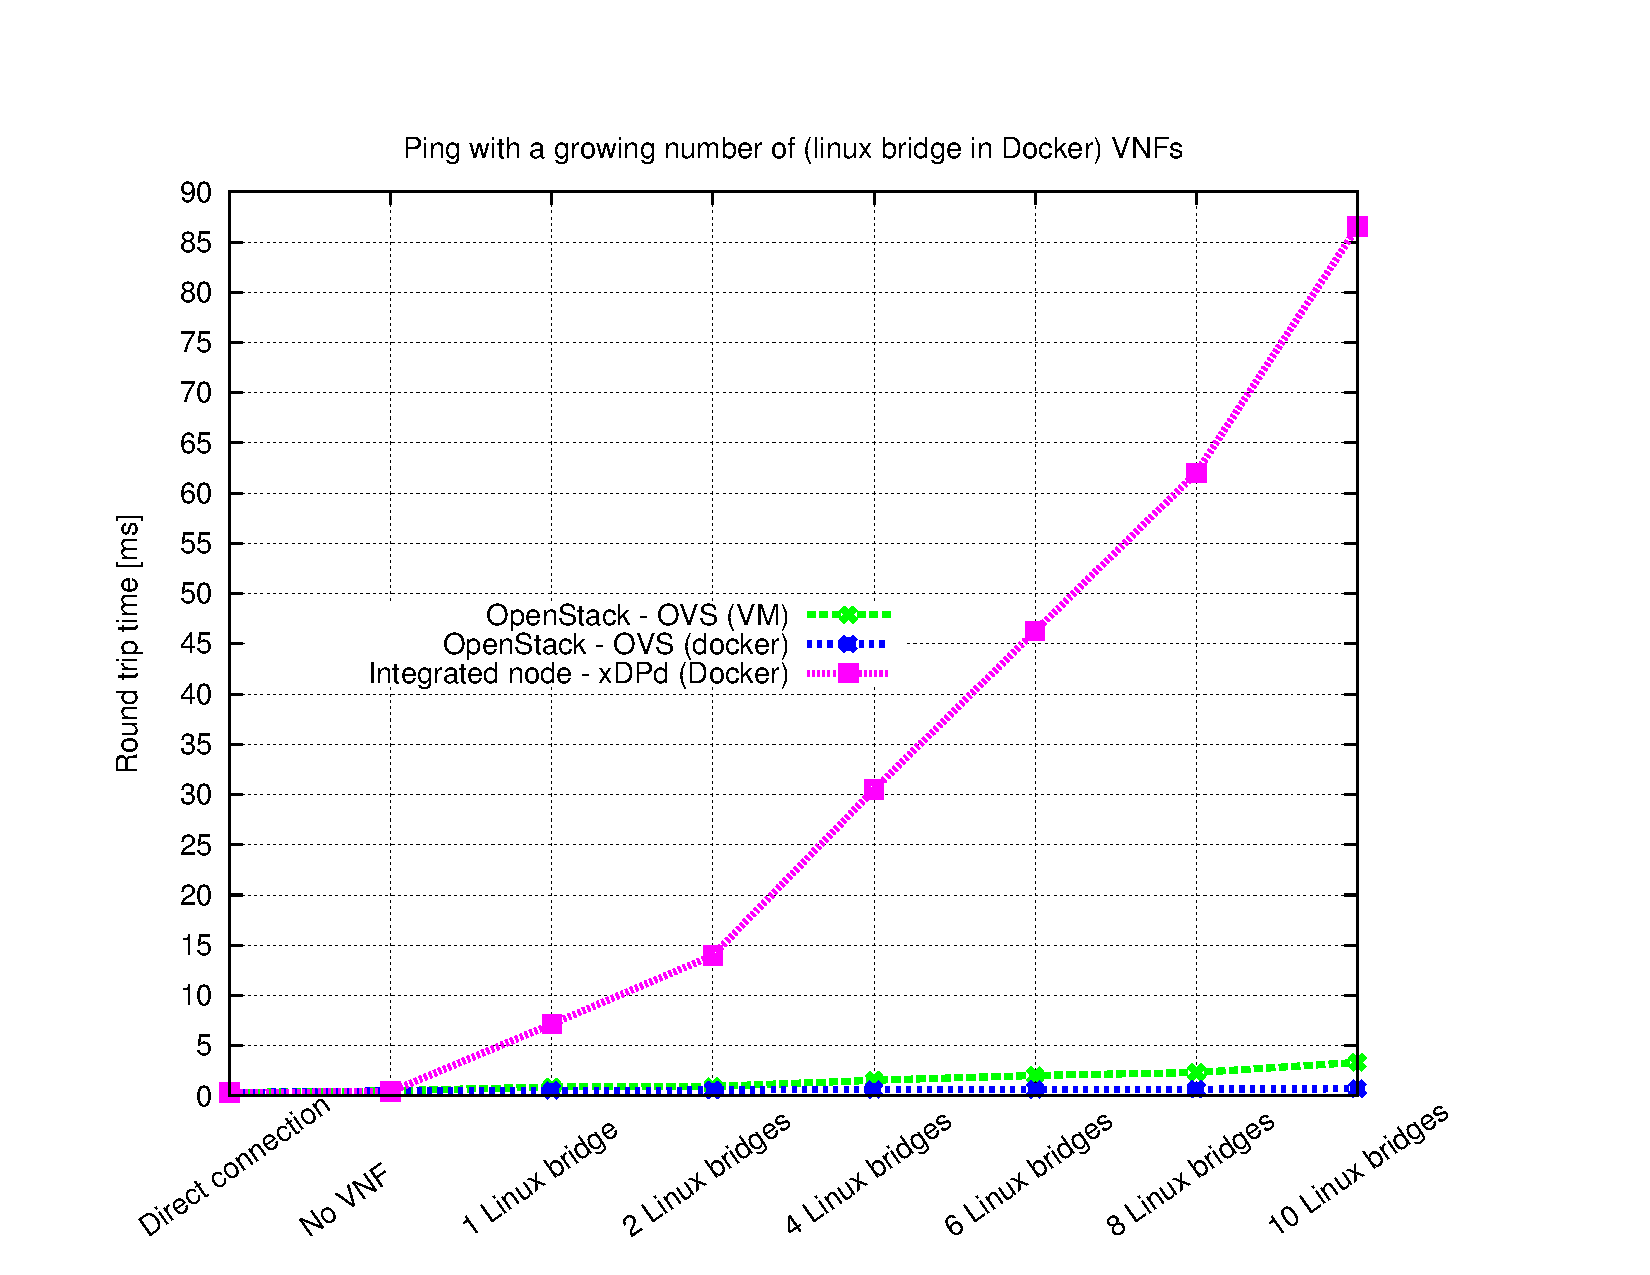
\includegraphics[clip= true, width= 0.5\columnwidth]{images/graphs/ping.pdf}
		}%
		\subfloat[Througput TCP - \textit{wget}.]{%
			\label{fig:end_test2}
			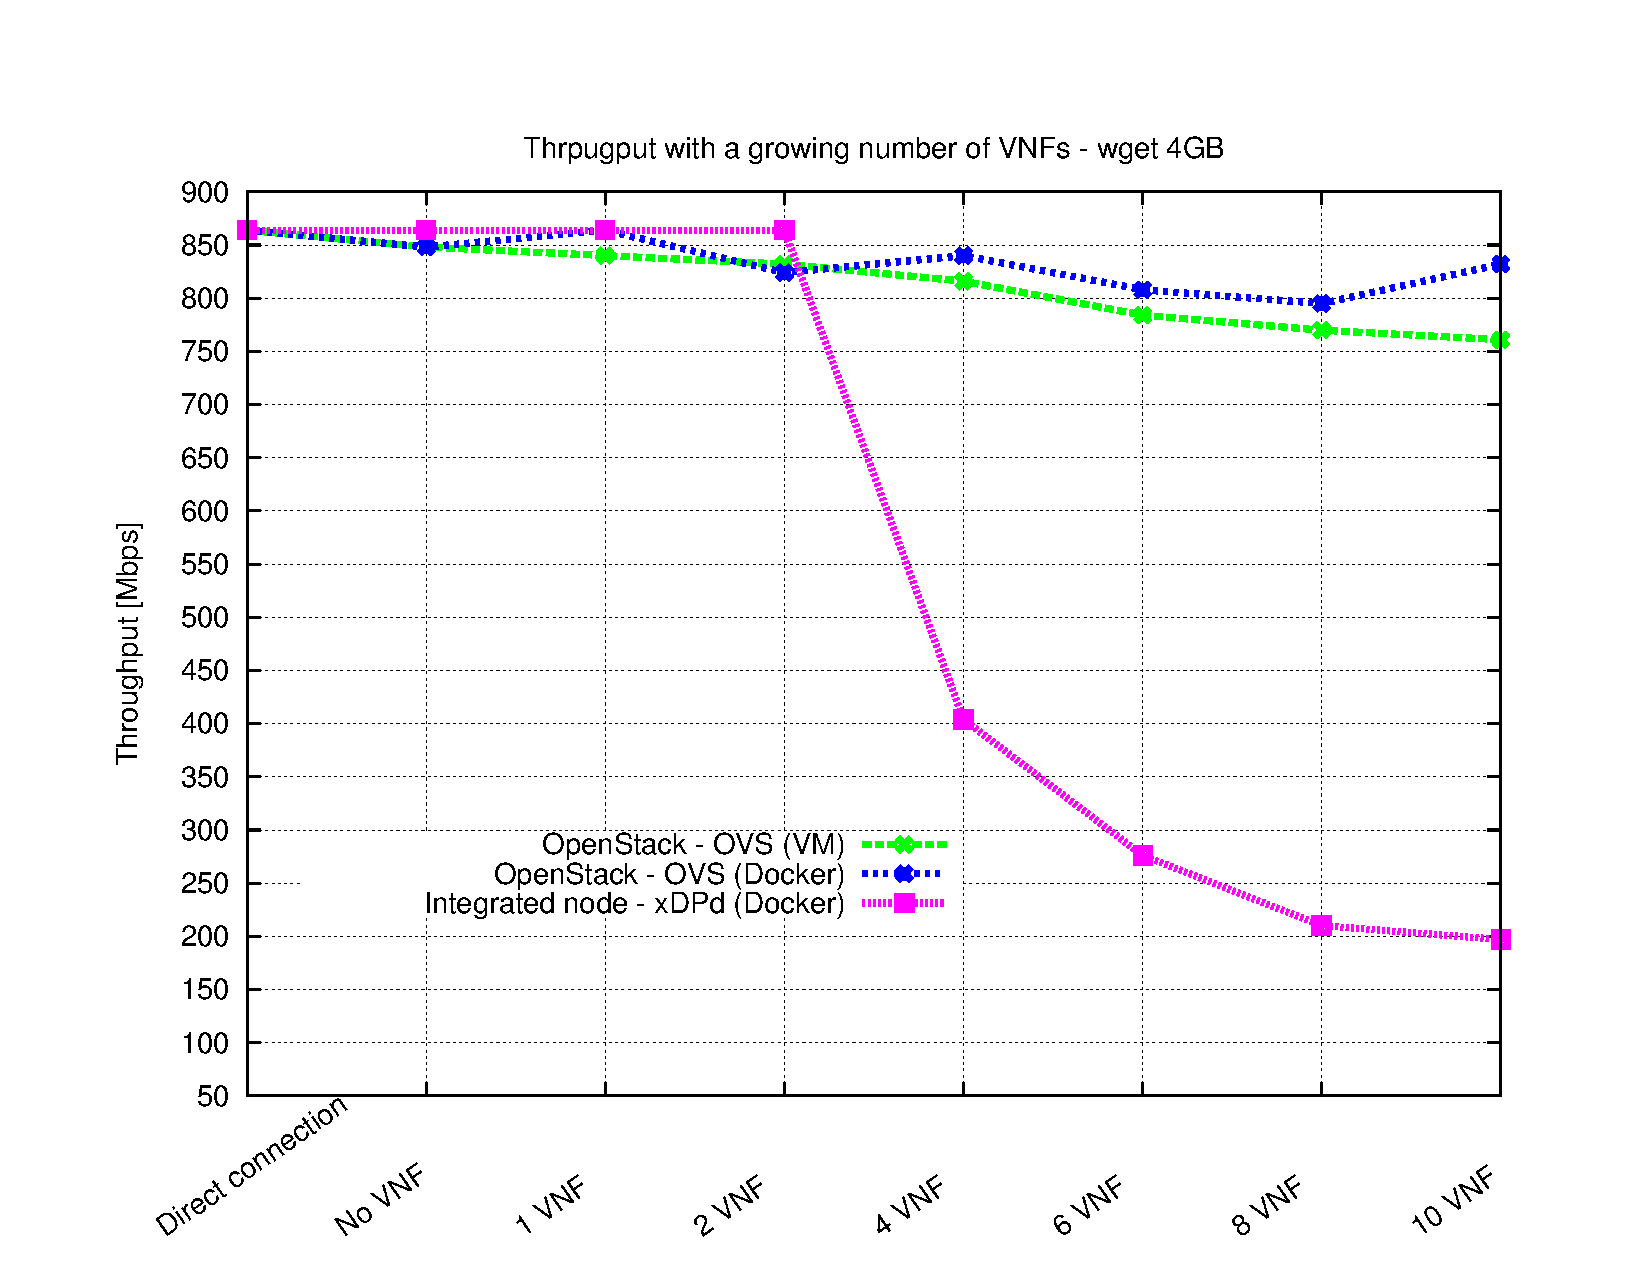
\includegraphics[clip= true, width= 0.5\columnwidth]{images/graphs/tcp_wget_throughput.pdf}
		}\\ %  ------- End of the first row ----------------------%
		\subfloat[Througput TCP - \textit{iperf}.]{%
			\label{fig:end_test3}
			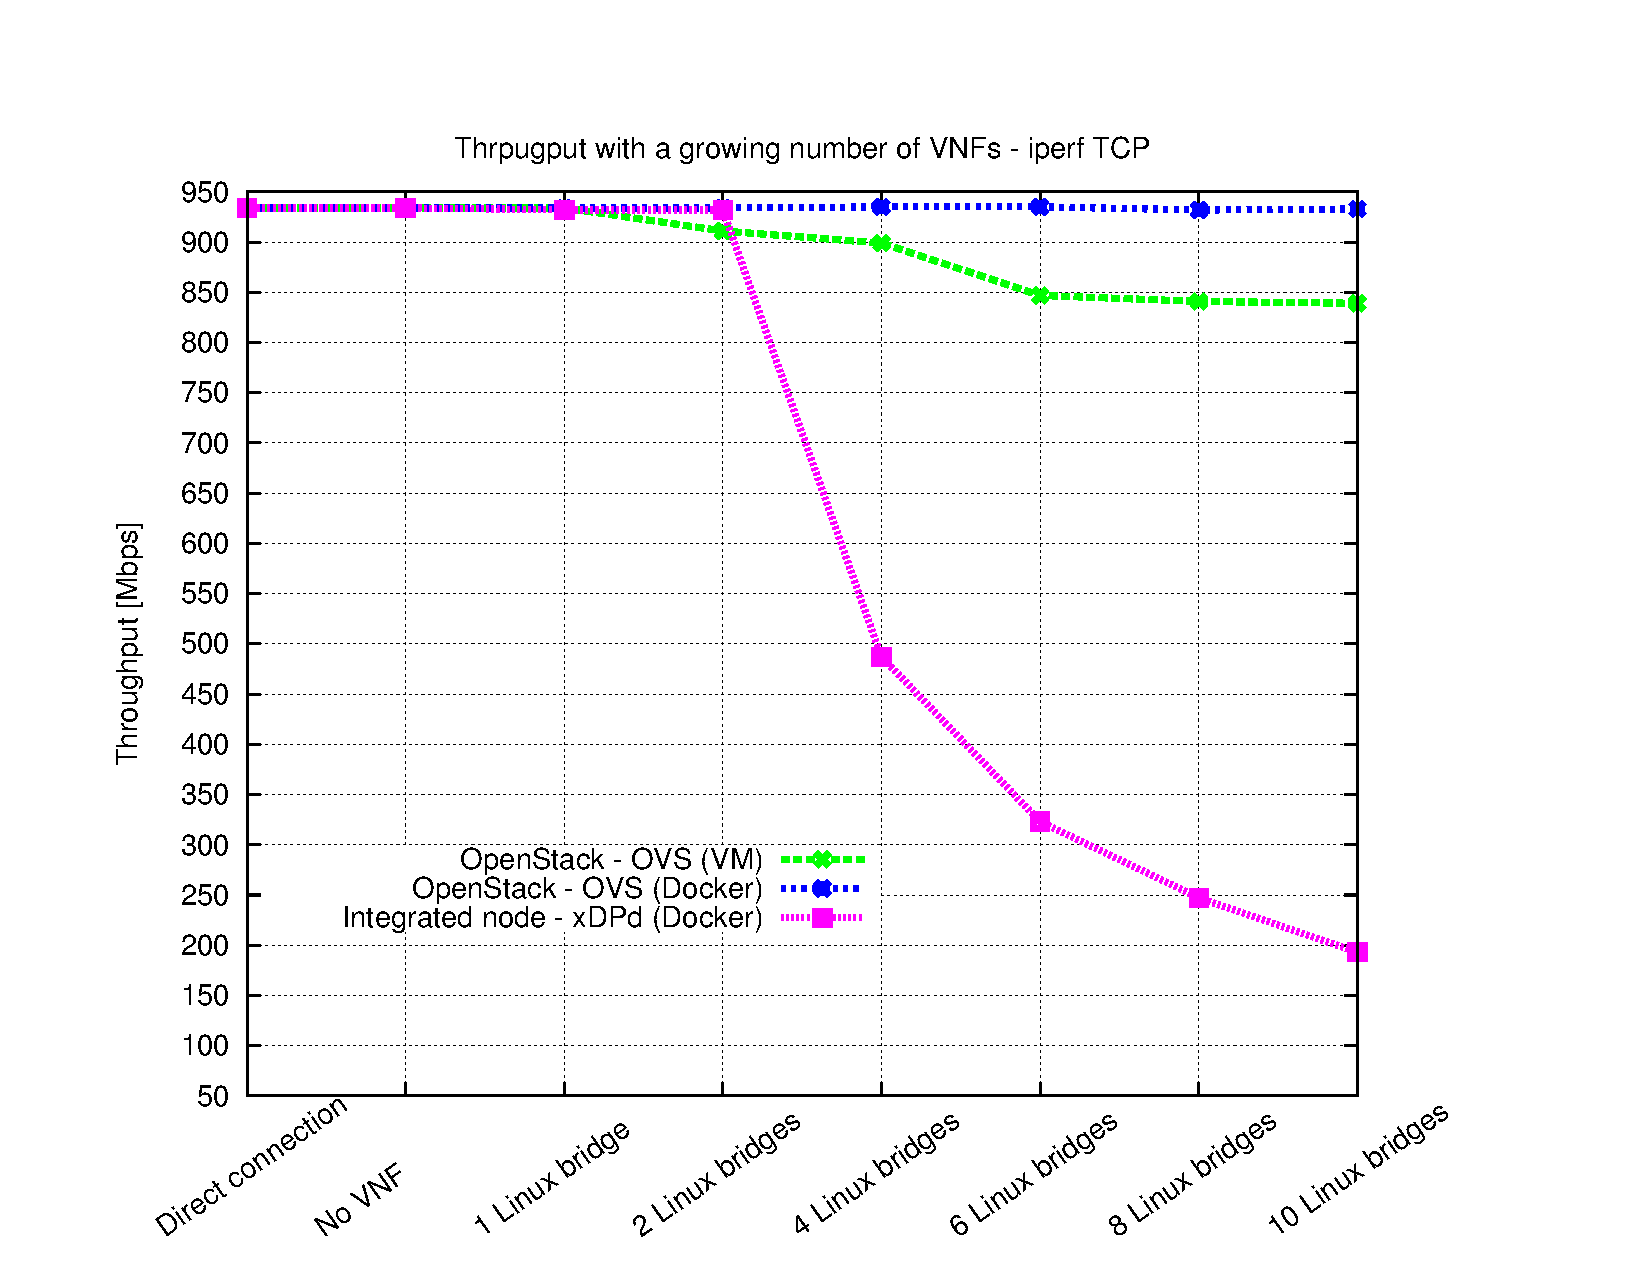
\includegraphics[clip= true, width= 0.5\columnwidth]{images/graphs/tcp_iperf_throughput.pdf}
		}%
		\subfloat[Througput UDP - \textit{iperf}.]{%
			\label{fig:end_test4}
			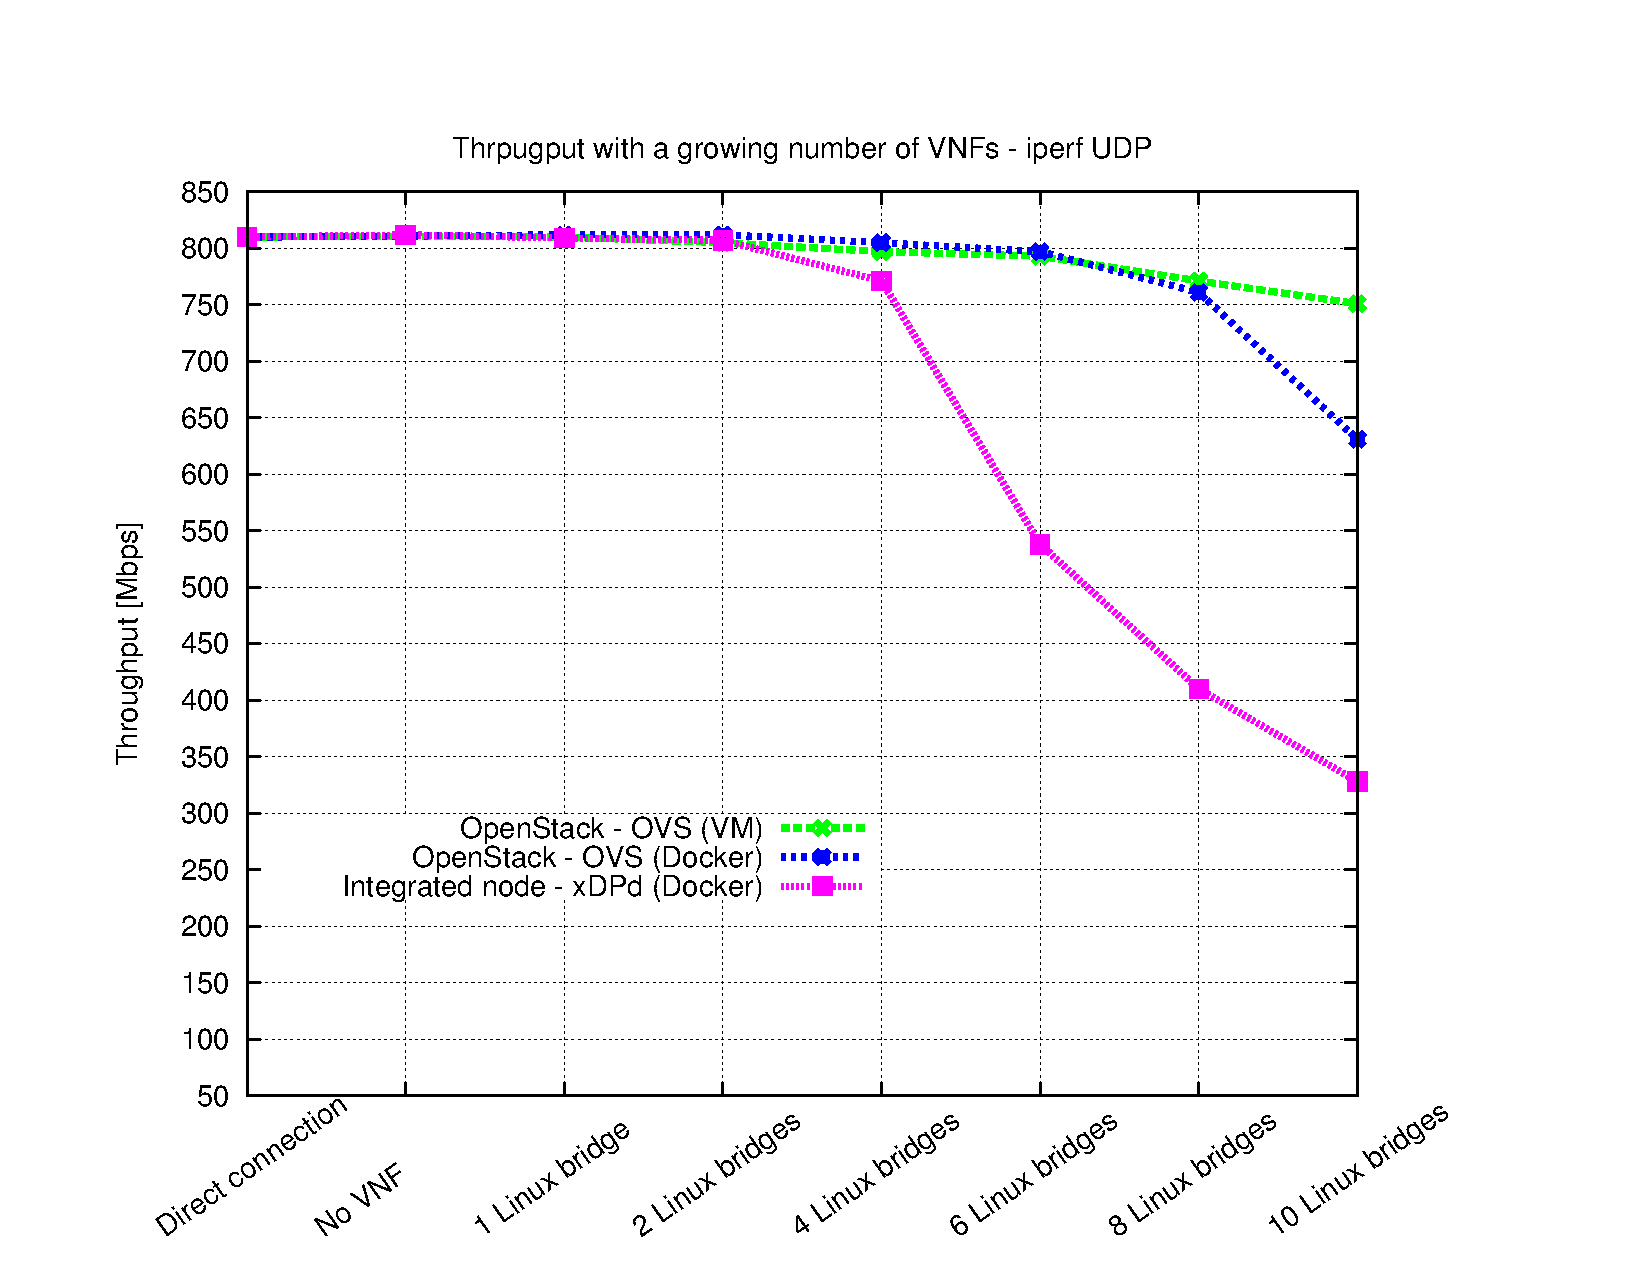
\includegraphics[clip= true, width= 0.5\columnwidth]{images/graphs/udp_throughput.pdf}
		}%
	\end{center}
	\caption{Performance tests. }
	\label{fig:performance_tests}
\end{figure*}

As expected, the deployment of a SG on the network does not come for free, since the results obtained are lower with respect to the case in which no service is instantiated between the user device and the server.
However, as evident by a comparison between line \texttt{\#1}, \texttt{\#2} and \texttt{\#3} of the table, this penalty is limited when the graph is deployed on an OpenStack-based node that use VMs, and almost zero when we use an OpenStack-based node using Docker containers.

Instead, when the user graph is scheduled in the integrated node (line \texttt{\#4}), performance are worse in all tests evaluated.



% !TEX root = ../thesis.tex
\chapter{Conclusion and future works}
\label{chap:Conclusions}
\label{sec:conclusion}

This thesis presents a network orchestration architecture that, starting from the service required by external actors (e.g., end users, Internet providers), takes care of instantiating it on the physical infrastructure of the network, by exploiting the opportunities offered by the Network Functions Virtualization (NFV) and Software Defined Networking (SDN) paradigm.


The contribution of this thesis is twofold. First, we proposed a new formalism, called \textit{service graph (SG)}, to flexibly model end-to-end network services. 
The SG data-model describes how to deliver flexible network services, leveraging existing elements and the traffic steering primitives introduced by NFV/SFC. 
It is worth noting that this SG definition is completely compliant with NFV principles of abstract description of a Service, but enriches its traditional expressiveness to model legacy networks and services. 

The second contribution is made by the introduction of the \textit{forwarding graph (FG)} and all the ``lowering process'' that leads to the deployment of an optimized service. This process of translation is capable to adapt the service delivering to available resources of the underlying infrastructure; moreover, it is also able to detect specific capabilities of selected nodes adapting the infrastructure graph obtained as output. 

In order to validate our model, we implement the \textit{OpenStack-based node} prototype and we also tested the \textit{integrated node} for physical infrastructure.

%In order to validate our model, we implemented two prototypes for the physical infrastructure: the \textit{integrated node} and the \textit{OpenStack-based node}. 
While the latter consists of a single server mainly based on ad hoc components, the former is implemented as a cluster of server orchestrated by the an extended version of the OpenStack framework.
Experimental results showed that, while the integrated node has low requirements in terms of memory, its performance are overcome by the OpenStack-based node in almost all the tests carried out except for tests about the deployment time, despite they are not so good are even better that the OpenStack-based results. The time of startup of the service is definitely the largest showed by the experimental results, because an user cannot wait that times for access their services.

As a plan for the future, we foresee two different challenges to be pursued in order to let this architecture to properly scale to the ISP network size. 
First, the proposal of an algorithm to implement a network-aware and resources-aware scheduling, capable of deploying VNFs on the nodes of the physical infrastructure by considering the paths expressed into the graph and also the features and the current usage of resources in single node (or domain). This require in the orchestrator the ability of splitting a single graph in multiple subgraphs and the instantiation of these in different nodes.
Second, the definition of a hierarchical orchestration layer would be expedient in order to be able to scale out to potentially the whole ISP network. 
This would allow the deployment of a FG across multiple administrative domains, in which the lower level orchestrators expose only some information to the upper level counterparts. 
This scenario is perfectly compatible with our architecture and will be object of further analysis; in fact, the global orchestrator presented in the thesis has syntactically identical northbound and southbound interfaces (in fact, it receives a FG from the service layer, and it is able to provide a FG to the next component), and hence a hierarchy of orchestrators is possible. 

To conclude, in the \textit{OpenStack-based node} we would have to get rid of \textit{network node} that force all outbound traffic from OpenStack to go from a router/nat positioned on node where \textit{network node} is installed,  which potentially affect the performance of our prototype.


%\appendix
% INCLUSIONE APPENDICI - - PERSONALIZZARE - TENERE COERENTE CON LISTA IN ALTO
%% !TEX root = ../thesis.tex
\chapter{An appendix}
\label{app:a}

appendix


%%%%%%%%%%%%%%%%%%%%%%%%%%%%%%%%%%%%%%%%%%%%%%%%%%%%%%%%%%%%%%%

% BIBLIOGRAFIA
\addcontentsline{toc}{chapter}{\refname}
\nocite{*}
\printbibliography

\end{document}